\documentclass[12pt, oneside, a4paper]{book}
% \documentclass[12pt, a4paper]{report}
\usepackage[export]{adjustbox}

\usepackage[x11names]{xcolor} % Load xcolor with X11 color names
% Define a custom dark green color
\definecolor{DarkGreen}{RGB}{0, 210, 0}
\definecolor{black}{RGB}{10, 10, 10}
\definecolor{Blue}{RGB}{1, 152, 252}

\usepackage{url}
\usepackage{algorithm}
\usepackage{algpseudocode}

\usepackage{geometry}
\usepackage{subcaption}
\usepackage{graphicx}

\usepackage{background}
 \backgroundsetup{contents={}}

\usepackage{placeins}
\usepackage{ragged2e}
\usepackage{multicol}
\usepackage{xcolor}
\usepackage{indentfirst}
\usepackage{booktabs}
\usepackage{multirow}
\usepackage{setspace}
\usepackage{rotating}
\usepackage{enumerate}
\usepackage{pgfplots}


\usepackage[utf8]{inputenc}
\usepackage{amsmath}
\usepackage{enumitem}
\usepackage{hyperref}
\usepackage{cite}

\usepackage{blindtext}

\graphicspath{graphics}
\tolerance=1
\emergencystretch=\maxdimen
\hyphenpenalty=10000
\hbadness=10000
\pagenumbering{gobble}

\newsavebox{\savefig}
\begin{document}
\newgeometry{top=6em, bottom=2em}
\begingroup
    \centering
    \large \textcolor{black}{A PROJECT REPORT ON}\\
    \Large \color{DarkGreen}\textbf{`` A COMPARATIVE STUDY OF VARIOUS IMAGE CLASSIFICATION MODELS AND THEIR INTERPRET-ABILITY USING THE PLANT VILLAGE DATASET ''}
    \color{black}
    \par\vspace{1em}
    
    \textcolor{Blue}{\normalsize \textit{SUBMITTED IN PARTIAL FULFILMENT OF THE REQUIREMENTS FOR THE AWARD OF THE DEGREE OF}} \\[1em]
    \color{red}\large\textbf{BACHELOR OF ENGINEERING (B.E.)} \\
    \color{red}\large\textbf{IN} \\
    \color{red}\large\textbf{COMPUTER SCIENCE AND ENGINEERING (2020-2024)}\\ [2em]
\endgroup

\begingroup
    \begin{center}
        \large \textcolor{DarkGreen}{\underline{\textbf{Submitted By:}}}\\
        \large \textcolor{Blue}{\textbf{Devraj Thokchom}}\\
        \normalsize MU Roll No: \textbf{202009}\\
        \large \textcolor{Blue}{\textbf{Deedal Wahengbam}}\\
        \normalsize MU Roll No: \textbf{202013}\\
        \large \textcolor{Blue}{\textbf{Lenin Khangjrakpam}}\\
        \normalsize MU Roll No: \textbf{204036}\\ [2em]
    \end{center}
    
    \begin{center}
        \large \textcolor{DarkGreen}{\underline{\textbf{Under the Guidance of:}}}\\
        \large \textcolor{Blue}{\textbf{Dr. Th Ibungomacha Singh}}\\
        \normalsize \textbf{Head of Department, CSE}\\
        \normalsize Manipur Institute of Technology\\ [1em]
    \end{center}
\endgroup

\begingroup
    \begin{center}
        
\includegraphics[scale=0.4]{graphics/MU Logo.png}\\[0.5em]
        \color{red}\large \textbf{DEPARTMENT OF COMPUTER SCIENCE AND ENGINEERING}\\
        \color{black}\normalsize \textit{(A Constituent College of Manipur University)}\\
        \color{red}\textbf{\large MANIPUR INSTITUTE OF TECHNOLOGY}\\
        \large \textbf{CANCHIPUR, MANIPUR, 795004}
    \end{center}
\endgroup
\restoregeometry
\newgeometry{top=10em, bottom=5em}

% ----------------Tile Start----------------------------------------

\newpage
    \begin{center}
        \large \textbf{A COMPARATIVE STUDY OF VARIOUS IMAGE CLASSIFICATION MODELS AND THEIR INTERPRET-ABILITY USING THE PLANT VILLAGE DATASET} \\
        \vspace{1em}
        \large $\text{Devraj Thokchom}^1$ \space \space \space $\text{Deedal Wahengbam}^2$ \space \space \space $\text{Lenin Khangjrakpam}^3$ \par
        \vspace{0.5em}
        August 2024  
    \end{center}

    \vspace*{\fill}
    \par\vspace{-.5\ht\strutbox}\noindent\hrulefill\\
    ${}^{[1]} \text{Manipur Institute of Technology (MIT) and devrajthok@gmail.com}$\\
    ${}^{[2]} \text{Manipur Institute of Technology (MIT) and deedalwahengbam005@gmail.com }$\\
    ${}^{[3]} \text{Manipur Institute of Technology (MIT) and leninkhangjrakpam@gmail.com}$\\
    



% -------------- Certificate -------------
\newpage
\backgroundsetup{
contents={
\includegraphics{graphics/MU Logo.png}},
    angle=0,
    scale=1,
    opacity=0.1
}
\begingroup
    \begin{center}
        \textcolor{black}
        {
        \color{red}\large \text{DEPARTMENT OF COMPUTER SCIENCE \& ENGINEERING}\\
        \normalsize \textbf{MANIPUR INSTITUTE OF TECHNOLOGY}\\
        \normalsize Canchipur, IMPHAL, 795004\\[1em]
        
\includegraphics[scale=0.4]{graphics/MU Logo.png}\\[0.5em]
        }
        \textcolor{red}
        {
        \large \textit{\underline{\textbf{CERTIFICATE}}}
        }
    \end{center}
\endgroup

\begingroup
    \begin{onehalfspace}
  \color{black}
  \textit{This is to certify that the project entitled \textbf{``A Comparative Study of Various Image Classification Models and their Interpret-Ability using the Plant Village Dataset''} is a genuine work done by}\\[1em]
    \textit{\hspace*{4em}\textbf{Mr. Devraj Thokchom}, MU Roll No: \textbf{202009}\\
    \hspace*{4em}\textbf{Mr. Deedal Wahengbam}, MU Roll No: \textbf{202013}\\
    \hspace*{4em}\textbf{Mr. Lenin Khangjrakpam}, MU Roll No: \textbf{204036}}\\[1em]

    \indent \textit{students of \textbf{B.E.} from \textbf{Manipur Institute of Technology} under my guidance and supervision. This project has not been submitted to any other examination and does not form part of any other project undertaken by the candidate.}\\
    \indent \textit{I hereby forward this project work for the partial fulfillment of the requirements for the award of the degree of \textbf{Bachelor of Engineering in Computer Science and Engineering, 2024.}\\
    I wish them all success in life.}
    \end{onehalfspace}
\endgroup

\vspace{7em}

\begingroup
       \begin{flushright}
        \begin{minipage}{0.6\textwidth}
            \centering
            \color{black}Head of Department \& Internal Project Guide \\
            \vspace{1em}
            \color{orange}\textbf{(Th. Ibungomacha Singh)} \\
           \color{green} Department of Computer Science \& Engineering\\
        \end{minipage}
    \end{flushright}
\endgroup

%  ------------- Certificate 2 ------------------------------
\newpage
\backgroundsetup{
contents={
\includegraphics{graphics/MU Logo.png}},
    angle=0,
    scale=1,
    opacity=0.1
}
\begingroup
    \begin{center}
        \textcolor{black}
        {
        \color{red}\large \text{DEPARTMENT OF COMPUTER SCIENCE \& ENGINEERING}\\
        \normalsize \textbf{MANIPUR INSTITUTE OF TECHNOLOGY}\\
        \normalsize Canchipur, IMPHAL, 795004\\[1em]
        
\includegraphics[scale=0.4]{graphics/MU Logo.png}\\[0.5em]
        }
        \textcolor{red}
        {
        \large \textit{\underline{\textbf{CERTIFICATE OF APPROVAL}}}
        }
    \end{center}
\endgroup

\begingroup
    \begin{onehalfspace}
  \color{black}
  \textit{This is to certify that the project entitled \textbf{``A Comparative Study of Various Image Classification Models and their Interpret-Ability using the Plant Village Dataset''} is a genuine work done by}\\[1em]
    \textit{\hspace*{4em}\textbf{Mr. Devraj Thokchom}, MU Roll No: \textbf{202009}\\
    \hspace*{4em}\textbf{Mr. Deedal Wahengbam}, MU Roll No: \textbf{202013}\\
    \hspace*{4em}\textbf{Mr. Lenin Khangjrakpam}, MU Roll No: \textbf{204036}}\\[1em]

    \textit{Further certified that no part of this project constitutes any part of a book or a journal already published elsewhere for the award of any other Degree of Bachelor of Engineering Department of the Institute.}\par
    \textit{I wish them all success in their academic endeavor.}\par
    \end{onehalfspace}
\endgroup

\vspace{7em}

\begingroup
    \begin{minipage}[c]{.5\textwidth}
    \RaggedRight
    \large Date.....  \par
    \large Place.....  \par
    \end{minipage}%
    \begin{minipage}[c]{.5\textwidth}
    \RaggedRight
    \normalsize \textbf{Signature of Examiner}\\
    \end{minipage}    
\endgroup

% -------------- Undertaking Start ----------------------------------
\newpage
\begingroup
    \begin{center}
        \textcolor{black}
        {
        \color{red}\large \text{DEPARTMENT OF COMPUTER SCIENCE \& ENGINEERING}\\
        \normalsize \textbf{MANIPUR INSTITUTE OF TECHNOLOGY}\\
        \normalsize Canchipur, IMPHAL, 795004\\[1em]
        
\includegraphics[scale=0.4]{graphics/MU Logo.png}\\[0.5em]
        }
        \textcolor{red}
        {
        \large \textit{\underline{\textbf{UNDERTAKING}}}
        }
    \end{center}
\endgroup

\begingroup
    \begin{onehalfspace}   
    \textit{
    We declare that the work presented in this project titled \textbf{``A Comparative Study of Various Image Classification Models and their Interpret-Ability using the Plant Village Dataset''} submitted to the \textit{Department of Computer Science \& Engineering, Manipur Institute of Technology}, for the fulfilment of the requirement of Bachelor of Engineering in Computer Science \& Engineering, is our original work. We have not plagiarized or submitted the same work for the award of any other degree. When we used external resources, we commit to properly citing all sources of such resources in our project to give due credit to the original authors. Any external content used has been appropriately referenced in accordance with academic standards. In case this understanding is found incorrect, we accept that our degree may be unconditionally withdrawn.}\\[1em]
    \textit{\hspace*{4em}\textbf{Mr. Devraj Thokchom}, MU Roll No: \textbf{202009}\\
    \hspace*{4em}\textbf{Mr. Deedal Wahengbam}, MU Roll No: \textbf{202013}\\
    \hspace*{4em}\textbf{Mr. Lenin Khangjrakpam}, MU Roll No: \textbf{204036}}\\[1em]

    
    \end{onehalfspace}
\endgroup

\vspace{7em}

\begingroup
       \begin{flushright}
        \begin{minipage}{0.6\textwidth}
            \centering
            Head of Department \& Internal Project Guide \\
            \vspace{1em}
            \textcolor{orange}{(Th. Ibungomacha Singh) \\}
            \textcolor{green}{Department of Computer Science \& Engineering}
        \end{minipage}
    \end{flushright}
\endgroup

% -------------- Undertaking End ----------------------------------
% --------------------------   Declaration Start ------------
\newpage
\begingroup
    \begin{center}
        \textcolor{black}
        {
        \color{red}\large \text{DEPARTMENT OF COMPUTER SCIENCE \& ENGINEERING}\\
        \normalsize \textbf{MANIPUR INSTITUTE OF TECHNOLOGY}\\
        \normalsize Canchipur, IMPHAL, 795004\\[1em]
        
\includegraphics[scale=0.4]{graphics/MU Logo.png}\\[0.5em]
        }
        \textcolor{red}
        {
        \large \textit{\underline{\textbf{DECLARATION}}}
        }
    \end{center}
\endgroup


\begingroup
    \justifying
    \textit{
    \color{black}\normalsize We, \textbf{Devraj Thochom (202009), Deedal Wahengbam (202013)} and \textbf{Lenin Khangjrakpam (204036)}, students  of Bachelor of Engineering in Computer Science and Engineering of Manipur Institute of Technology, hereby declare that the project entitled \textbf{\textit{``A Comparative Study of Various Image Classification Models and their Interpret-ability using the Plant Village dataset''}} has been carried out independently at the Institute under the guidance of \textbf{Professor Th Ibungomacha}, Head of Department (HOD) of Computer Science and Engineering.}
    \par\vspace{1em}
    \textit{We hereby declare that the work submitted in the thesis is our own, except where acknowledged in the text and has not been previously submitted for the award of the degree of Manipur Institute of Technology.}
    \par \vspace{12em}
\endgroup

\begingroup
    \begin{minipage}[c]{.5\textwidth}
    \RaggedRight
    \large Date.....  \par
    \large Place.....  \par
    \end{minipage}%
    \begin{minipage}[c]{.5\textwidth}
    \RaggedRight
    \normalsize \textbf{Deedal Wahengbam}\\
    \normalsize \textbf{Devraj Thokchom}\\
    \normalsize \textbf{Lenin Khangjrakpam}\\
    \end{minipage}    
\endgroup

% ----------- Acknowledgement Start ---------------
\newpage
\begingroup
    \begin{center}
        \textcolor{black}
        {
        \color{red}\large \text{DEPARTMENT OF COMPUTER SCIENCE \& ENGINEERING}\\
        \normalsize \textbf{MANIPUR INSTITUTE OF TECHNOLOGY}\\
        \normalsize Canchipur, IMPHAL, 795004\\[1em]
        % 
\includegraphics[scale=0.4]{graphics/MU Logo.png}\\[0.5em]
        }
        \textcolor{red}
        {
        \large \textit{\underline{\textbf{ACKNOWLEDGEMENT}}}
        }
    \end{center}
\endgroup


\begingroup
    \justifying
     \textit{\color{black}\normalsize First and Foremost, we would like to express our deepest gratitude to \textbf{Professor Th Ibungomacha}, Head of Department (HOD) of Computer Science and Engineering, Manipur Institute of Technology for his valuable advice, guidance, and for providing us the opportunity to carry out our project entitled: \textit{\textbf{A Comparative Study of Various Image Classification Models and their Interpret-ability using the Plant Village dataset}}.}
    \par \vspace{0.5em}
    \textit{\normalsize We are also thankful to \textbf{Professor N Basanta Singh}, Principal, Manipur Institute of Technology, for providing us the opportunity to undergo our project in Manipur Institute of Technology.}\par \vspace{0.5em}
    \normalsize \textit{We express our deep sense of gratitude and thanks to all other staff members for their keen interest and help in our project development.}\par \vspace{0.5em}
    \normalsize \textit{We are also thankful to our colleagues for their kind co-operation by giving us inspiration and encouragement throughout the development of this project.}\par \vspace{12em}
\endgroup

\begingroup
    \begin{minipage}[c]{.5\textwidth}
    \RaggedRight
    \large Date.....  \par
    \large Place.....  \par
    \end{minipage}%
    \begin{minipage}[c]{.5\textwidth}
    \RaggedRight
    \normalsize \textbf{Deedal Wahengbam}\\
    \normalsize \textbf{Devraj Thokchom}\\
    \normalsize \textbf{Lenin Khangjrakpam}\\
    \end{minipage}    
\endgroup

% ------ Acknowledgement end --------------------


% \begingroup
%     \centering
%     \color{red}\LARGE \textbf{ACKNOWLEDGEMENT}\par \vspace{1em}
%     \justifying
%     \color{black}\large First and Foremost, we would like to express our deepest gratitude to \textbf{Professor Th Ibungomacha}, Head of Department (HOD) of Computer Science and Engineering, Manipur Institute of Technology for his valuable advice, guidance, and for providing us the opportunity to carry out our project entitled: \textit{\textbf{A Comparative Study of Various Image Classification Models and their Interpret-ability using the Plant Village dataset}}.
%     \par \vspace{0.5em}
%     \large We are also thankful to \textbf{Professor N Basanta Singh}, Principal, Manipur Institute of Technology, for providing us the opportunity to undergo our project in Manipur Institute of Technology.\par \vspace{0.5em}
%     \large We express our deep sense of gratitude and thanks to all other staff members for their keen interest and help in our project development.\par \vspace{0.5em}
%     \large We are also thankful to our colleagues for their kind co-operation by giving us inspiration and encouragement throughout the development of this project.\par \vspace{12em}
% \endgroup

% \begingroup
%     \begin{minipage}[c]{.5\textwidth}
%     \RaggedRight
%     \large Date.....  \par
%     \large Place.....  \par
%     \end{minipage}%
%     \begin{minipage}[c]{.5\textwidth}
%     \RaggedRight
%     \normalsize \textbf{Deedal Wahengbam}\\
%     \normalsize \textbf{Devraj Thokchom}\\
%     \normalsize \textbf{Lenin Khangjrakpam}\\
%     \end{minipage}    
% \endgroup


\newpage
% \NoBgThispage
\backgroundsetup{contents={}}
\begingroup
    \begin{center}
        \LARGE \textbf{ABSTRACT}\\
    \end{center}
    \justifying
    \normalsize In this study, we conduct a comprehensive comparative analysis of various image classification machine learning models using the Plant Village dataset, which we reduced to 11 distinct classes of plant diseases. Leveraging the power of transfer learning and fine-tuning, we evaluate three pre-trained CNN models—\textbf{VGG16, Xception, and MobileNetV2}—as base models. To further compare performance with nonneural network models, we utilize the pre-trained MobileNetV2 model as a feature extractor, training a \textbf{Support Vector Machine (SVM), K-Nearest Neighbors (KNN), Random Forest and Extreme Gradient Boosting (XGBoost)} classifiers on the extracted features. Our findings reveal that neural network-based models, particularly those using transfer learning, significantly outperform traditional classifiers in terms of accuracy.\par \vspace{1em}
    Additionally, we design and train a custom CNN model from scratch named \textbf{\textit{CNN10L}}, structured similarly to the VGG architecture, which, while achieving commendable accuracy, still falls short of the pre-trained models' performance. \par \vspace{1em}
    To gain deeper insights into the model's behavior, we also perform an in-depth analysis of the fine tuned (on Plant Village Dataset) VGG16-based model by visualizing its convolutional layers and interpreting the learned features. Techniques such as image masking and activation mapping are employed to understand the model's focus areas and decision-making process.\par \vspace{1em}
    To further interpret our CNN model, we also, perform visualization of the feature extracted by our model on a 2D and 3D feature space using \textbf{PCA and t-SNE}. We also used a \textbf{cosine similarity score} to find all the \textbf{\textit{N}} data instances that are nearest neighbors to a given/query feature vector (extracted from image)
 \par\vspace{1em}
    Our results underscore the efficacy of transfer learning in image classification tasks and provide a detailed comparison of different model architectures and classification approaches. This study not only highlights the superior performance of fine-tuned pre-trained models but also sheds light on the internal workings of CNNs through comprehensive visualization techniques.\par\vspace{1em}
    
    \large \textbf{Keywords:} \par \vspace{1em}
    \normalsize    Convolutional Neural Network, Transfer Learning, Fine Tuning, Plant Disease Classification, Image Classification, Plant Village Dataset, VGG16, MobileNetV2, Xception, CNN10L, CNN Model Interpretation, Support Vector Machine (SVM), K-Nearest Neighbors (KNN), Random Forest,  Extreme Gradient Boosting (XGBoost), Feature Extraction, Model Performance Comparison, Cosine Similarity, PCA, t-SNE, Agricultural Technology
\endgroup

% Create the table of contents
\tableofcontents

\listoftables
\listoffigures 


\chapter{Introduction}
\pagenumbering{arabic}

\section{Background}
Machine Learning is a field of Artificial Intelligence that focuses on developing algorithms and models, by learning from patterns in a dataset and using it to make predictions on new data. These algorithms can be very useful for identifying patterns and relationships in a given database, which can be invaluable to extract insights or make predictions without being explicitly programmed.\par \vspace{1em}
Machine Learning can be classified into various categories; supervised learning, unsupervised learning, and reinforcement learning being the most common ones. Supervised Learning Algorithms learn from labelled data, making predictions based on the given data. Unsupervised Learning Algorithms learn from unlabelled data, where the algorithm identifies patterns and structures within the data. Reinforcement Learning Algorithms learns through interacting with an environment, and aiming to maximize cumulative rewards.\par \vspace{1em}
Convolutional Neural Networks or CNNs are a subset of deep learning models especially useful for tasks involving processing of visual data. Its architecture is particularly inspired by the connectivity patterns of the human brain, especially the visual cortex. Its primary goal is to automatically learn the hierarchical representations of features directly from raw data.\par \vspace{1em} \newpage
CNNs use specialized architectures that incorporate convolutional layers, pooling layers, and fully connected layers. Convolutional layers apply convolution operations to the input image, using learnable filters to extract features such as edges, textures, or shapes. Pooling layers then reduce the spatial dimensions of the feature maps generated by the convolutional layers, helping to decrease computational complexity and control overfitting. Finally, fully connected layers use the extracted features to classify the input image into various categories.\par \vspace{1em}

\section{Problem Statement}

Accurate and efficient detection of plant diseases is critical for ensuring food security and agricultural productivity. Traditional methods of plant disease identification often rely on expert knowledge and manual inspection, which can be time-consuming, labor-intensive, and prone to human error. With the advent of deep learning and advanced machine learning techniques, there is a growing potential to automate and enhance the accuracy of disease classification using image-based analysis.\par
The Plant Village dataset provides a robust foundation for developing machine learning models aimed at identifying various plant diseases from images. However, the challenge lies in selecting and optimizing the appropriate model architectures to achieve high classification accuracy. While Convolutional Neural Networks (CNNs) have shown great promise in image recognition tasks, there is a need to systematically compare their performance with traditional classifiers and evaluate the benefits of using transfer learning and fine-tuning techniques with pre-trained models.\par

This study aims to address the following key questions:
\begin{enumerate}
    \item How do pre-trained models like VGG16, Xception, and MobileNetV2 perform in the context of plant disease classification when fine-tuned on the Plant Village dataset?
    \item Can traditional classifiers such as SVM, KNN, Random Forest, and XGBoost, when used with features extracted from pre-trained models, achieve comparable performance to CNN-based models?
    \item What is the effectiveness of a custom-designed CNN model in classifying plant diseases compared to fine-tuned pre-trained models?
    \item How can we interpret and visualize the features learned by CNN models to gain insights into their decision-making processes?
\end{enumerate}
\par

By addressing these questions, this research aims to identify the most effective machine learning approaches for plant disease classification and provide a deeper understanding of the underlying mechanisms of CNN models through visualization techniques. \par



\section{Scope of Study}
The scope of this study encompasses a comprehensive evaluation of various image classification machine learning models applied to the Plant Village dataset, specifically focusing on the detection and classification of plant diseases. The key components of this study are as follows:
\begin{enumerate}
    \item \textbf{Dataset Utilization:} \\
    The Plant Village dataset, consisting of images categorized into 11 different plant disease classes, is used to train and evaluate the models. This dataset provides a diverse and challenging testbed for assessing model performance in real-world scenarios.
    \item \textbf{Model Selection and Training:} 
    \begin{itemize}
        \item  Three pre-trained models, VGG16, Xception, and MobileNetV2, are employed as base models for transfer learning and fine-tuning. These models are chosen for their proven efficacy in image classification tasks and their ability to leverage pre-learned features from large datasets like ImageNet.
        \item In addition to these neural network models, traditional machine learning classifiers such as SVM, KNN, Random Forest, and XGBoost are trained using features extracted from the fine-tuned MobileNetV2 model. This provides a comparative analysis of deep learning models against conventional machine learning approaches.
    \end{itemize}
    \item \textbf{Model Development: }\\
    A custom Convolutional Neural Network (CNN) with 10 layers is designed and trained from scratch, inspired by the VGG architecture. This model serves as a baseline to compare the performance of transfer learning models and to understand the effectiveness of custom architectures on the dataset.
    \item \textbf{Model Interpretation and Analysis:} \\
    Various techniques are employed to interpret and analyze the models, including:
    \begin{itemize}
        \item Visualization of the first layer filters and feature maps at different layers.
        \item Comparative analysis of feature maps using normal and masked images.
        \item Feature space visualization using PCA and t-SNE before and after fine-tuning.
        \item Nearest neighbor search using cosine similarity to evaluate the feature representations.
        \item Saliency Map Generation
    \end{itemize}
    \item \textbf{Deployment:} \\
    The best-performing model is deployed using Flask to serve as an API for real-time image classification. The frontend of the application is developed using React Native, enabling users to submit images and receive predictions.
    \item \textbf{Performance Evaluation:} \\
    The models are evaluated based on their accuracy, confusion matrices, and interpretability. This includes a thorough comparison of the classification performance of neural network models and traditional classifiers.
\end{enumerate}


This study aims to provide a detailed comparative analysis of different machine learning models for plant disease classification, highlighting the strengths and limitations of each approach. By leveraging transfer learning, custom model development, and comprehensive model interpretation techniques, this study contributes valuable insights into the application of machine learning in agricultural disease detection.\par\vspace{1em}


\chapter{Literature Review}

In this chapter, we list all the papers, that we used to to perform our research work \par\vspace{1em}

\section{Literature Review}

\begin{enumerate}
    \item Konstantinos P. Ferentinos ( February 2018) \\
        \textbf{Deep learning models for plant disease detection and diagnosis} \\
        \href{https://www.sciencedirect.com/science/article/abs/pii/S0168169917311742}{https://www.sciencedirect.com/science/article/abs/pii/S0168169917311742} \\
         The paper develops neural network models to perform plant disease detection and diagnosis using simple leaves image of healthy and diseased leaves. Training used an open database of 87,848 images, containing 25 different plants, in a set of 58 different classes.Several model architectures were trained, with the best performance reaching a 99.53\% success rate in reaching the correct diagnosis
    
    \item Sharada Prasanna Mohanty, David Hughes, Marcel Salathé (2016) \\
        \textbf{Using Deep Learning for Image-Based Plant Disease Detection} \\
        \href{https://arxiv.org/abs/1604.03169}{https://arxiv.org/abs/1604.03169} \\
        The paper presents an innovative approach to addressing the significant issue of crop disease diagnosis by leveraging deep learning technology. The authors successfully trained a deep convolutional neural network on a large dataset of plant leaf images, achieving a high accuracy of 99.35\% in controlled conditions. However, the model's performance dropped to 31.4\% when tested with images from different sources, highlighting the need for more diverse training data. This study demonstrates the importance of improving data diversity to enhance model generalizability for real-world applications.
    
    \item Francois Chollet (2017) \\
        \textbf{Xception: Deep Learning with Depthwise Separable Convolutions} \\
        \href{https://doi.org/XXXXXX}{https://doi.org/XXXXXX} \\
        The paper introduces an interpretation of Inception modules in CNN as an intermediate step between regular convolution and depthwise separable convolution (a depthwise convolution followed by a pointwise convolution). By understanding depthwise separable convolution as an Inception module with a maximally large number of towers, the authors propose a new CNN architecture, Xception, which replaces Inception modules with depthwise separable convolutions.  \\
    
    \item Muhammad Hammad Saleem ,Johan Potgieter and Khalid Mahmood Arif (31 October 2019) \\
        \textbf{Plant Disease Detection and Classification by Deep Learning} \\
        \href{https://www.mdpi.com/2223-7747/8/11/468}{https://www.mdpi.com/2223-7747/8/11/468} \\
        This paper provides a comprehensive explanation of DL models used to visualize various plant diseases. In addition, some research gaps are identified from which to obtain greater transparency for detecting diseases in plants, even before their symptoms appear clearly.\\

    \item Muhammad Shoaib Shaker El-sappagh,Babar Shah,Akhtar Ali,Asad Ullah,Fayadh Alenezi,Tsanko Gechev,Tariq Hussain and Farman Ali (2023) \\
        \textbf{An advanced deep learning models-based plant disease detection: A review of recent research } \\
        \href{https://www.frontiersin.org/journals/plant-science/articles/10.3389/fpls.2023.1158933/full}{https://www.frontiersin.org/journals/plant-science/articles/10.3389/fpls.2023.1158933/full} \\
        This paper addresses the challenges and limitations associated with using ML and DL for plant disease identification, such as issues with data availability, imaging quality, and the differentiation between healthy and diseased plants. The research provides valuable insights for plant disease detection researchers, practitioners, and industry professionals by offering solutions to these challenges and limitations, providing a comprehensive understanding of the current state of research in this field, highlighting the benefits and limitations of these methods, and proposing potential solutions to overcome the challenges of their implementation.\\

    \item Edna Chebet Too , Li Yujian , Sam Njuki and Liu Yingchun(June 2019) \\
        \textbf{A comparative study of fine-tuning deep learning models for plant disease identification} \\
        \href{https://www.sciencedirect.com/science/article/abs/pii/S0168169917313303}{https://www.sciencedirect.com/science/article/abs/pii/S0168169917313303} \\
        This paper is a comparative study of state-of-the-art deep learning for plants disease detection using images of leaves. The results show that deeper models are not only accurate but have fewer number of parameters. DenseNet model also perform better than other models studied with no signs of overfitting and performance deterioration.\\

    \item Murk Chohan, Adil Khan, Rozina Chohan, Saif Hassan Katpar and Muhammad Saleem Mahar (May 2020) \\
        \textbf{Plant Disease Detection using Deep Learning} \\
        \href{https://www.researchgate.net/profile/Saif-Katper/publication/341025012_Plant_Disease_Detection_using_Deep_Learning/links/5eabf714299bf18b958a94a8/Plant-Disease-Detection-using-Deep-Learning.pdf}
        {https://www.researchgate.net/profile/Saif-Katper/publication/341025012 \_Plant \_Disease\_Detection\_using\_Deep\_Learning/links/5eabf714299bf18b958a94a8/Plant-Disease-Detection-using-Deep-Learning.pdf} \\
        This paper proposes a deep learning based model named plant disease detector. The model is able to detect several diseases from plants using pictures of their leaves. Plant disease detection model is developed using neural network. First of all augmentation is applied on dataset to increase the sample size. Later Convolution Neural Network (CNN) is used with multiple convolution and pooling layers. PlantVillage dataset is used to train the model. After training the model, it is tested properly to validate the results.

    \item Faye Mohameth, Chen Bingcai and Kane Amath Sada (June 2020) \\
        \textbf{Plant Disease Detection with Deep Learning and Feature Extraction Using Plant Village} \\
        \href{https://www.scirp.org/journal/paperinformation?paperid=100958}{https://www.scirp.org/journal/paperinformation?paperid=100958} \\
        This paper evaluates CNN’s architectures applying transfer learning and deep feature extraction. All the features obtained will also be classified by SVM and KNN. Our work is feasible by the use of the open source Plant Village Dataset. The result obtained shows that SVM is the best classifier for leaf’s diseases detection.
    
    \item Rasim Alguliyev, Yadigar Imamverdiyev, Lyudmila Sukhostat and Ruslan Bayramov  ( 01 September 2021) \\
        \textbf{Plant disease detection based on a deep model} \\
        \href{https://link.springer.com/article/10.1007/s00500-021-06176-4}{https://link.springer.com/article/10.1007/s00500-021-06176-4} \\
        This paper proposes an accurate approach to identify plant leaf diseases based on the deep convolutional neural network and gated recurrent units. The proposed model is trained to identify common plant leaf diseases of 14 species. The experimental results are compared to other well-known models. This study shows that the proposed model based on deep learning provides the best solution in the diagnosis of plant diseases with high accuracy, and that the gated recurrent unit neural network considered as a classifier can improve the accuracy of the convolutional neural network model. 

    \item Shima Ramesh, Ramachandra Hebbar,Niveditha M.,Pooja R., Prasad Bhat N., Shashank N., Vinod P.V. ( 2018) \\
        \textbf{Plant Disease Detection Using Machine Learning} \\
        \href{https://ieeexplore.ieee.org/abstract/document/8437085}{https://ieeexplore.ieee.org/abstract/document/8437085} \\
        This paper makes use of Random Forest in identifying between healthy and diseased leaf from the data sets created. Our proposed paper includes various phases of implementation namely dataset creation, feature extraction, training the classifier and classification. The created datasets of diseased and healthy leaves are collectively trained under Random Forest to classify the diseased and healthy images.
        
    \item \textbf{Laha Ale, Alaa Sheta, Longzhuang Li, Ye Wang, Ning Zhang} (2019 ) \\
        \textbf{Deep Learning Based Plant Disease Detection for Smart Agriculture} \\
        \href{https://ieeexplore.ieee.org/abstract/document/9024439}{https://ieeexplore.ieee.org/abstract/document/9024439} \\
        This paper proposes a Densely Connected Convolutional Networks (DenseNet) based transfer learning method to detect the plant diseases, which expects to run on edge servers with augmented computing resources. It then proposes a lightweight Deep Neural Networks (DNN) approach that can run on Internet of Things (IoT) devices with constrained resources.
    
\end{enumerate}



 
\chapter{Theoretical Background}
In this chapter, we  provide a theoretical background, concept require by the reader to understand our research work.
\par\vspace{1em}

\section{Convolutional Neural Network (CNN)}
    Convolutional neural networks (CNN) are a regularized type of feed-forward neural network that learns feature engineering by itself via filters (or kernel) optimization. \cite{convnet}
    \par\vspace{1em}
    
    \begin{figure}[h]
            \centering
            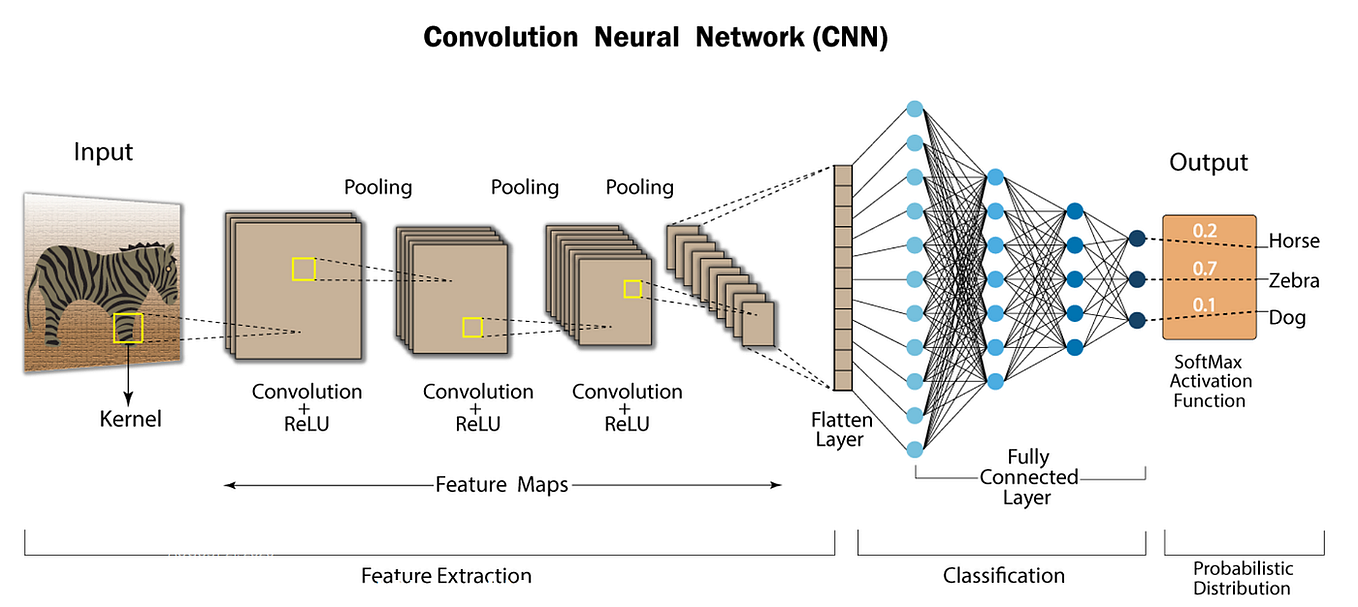
\includegraphics[width=1\textwidth]{graphics/chapter3/general cnn classification model.png}
            \caption{A typical ConvNet Classification Model, Source: \cite{convnet-fig}} 
            \label{fig:cnn1}
        \end{figure}
        
        
    \subsection{Architecture of CNN}
    A convolutional neural network consists of an input layer, hidden layers and an output layer. In a convolutional neural network, the hidden layers include one or more layers that perform convolutions. Typically this includes a layer that performs a dot product of the convolution kernel with the layer's input matrix. This product is usually the Frobenius inner product, and its activation function is commonly ReLU. As the convolution kernel slides along the input matrix for the layer, the convolution operation generates a feature map, which in turn contributes to the input of the next layer. This is followed by other layers such as pooling layers, fully connected layers, and normalization layers. Here it should be noted how close a convolutional neural network is to a matched filter\cite{convnet-1}.
        \subsubsection{Convolution Layers}
        In a CNN, the input is a tensor with shape:        
        \[(\text{number of inputs}) * (\text{input height}) * (\text{input width}) * (\text{input channels})\]
        After passing through a convolutional layer, the image becomes abstracted to a feature map, also called an activation map, with shape:
        \[(\text{number of inputs}) * (\text{feature map height}) * (\text{feature map width}) * (\text{feature map channels})\]
        \par \vspace{1em}
        Convolutional layers convolve the input and pass its result to the next layer. This is similar to the response of a neuron in the visual cortex to a specific stimulus\cite{convnet-2}. Each convolutional neuron processes data only for its receptive field.
        
        \subsubsection{Pooling Layers}
        Convolutional networks may include local and/or global pooling layers along with traditional convolutional layers. Pooling layers reduce the dimensions of data by combining the outputs of neuron clusters at one layer into a single neuron in the next layer. Local pooling combines small clusters, tiling sizes such as 2 × 2 are commonly used. Global pooling acts on all the neurons of the feature map.There are two common types of pooling in popular use: max and average. Max pooling uses the maximum value of each local cluster of neurons in the feature map, while average pooling takes the average value \cite{convnet-3}.
        
        \subsubsection{Fully Connected Layers}
        Fully connected layers connect every neuron in one layer to every neuron in another layer. It is the same as a traditional multilayer perceptron neural network (MLP). The flattened matrix goes through a fully connected layer to classify the image
        
        \subsubsection{Activation Function}
        Activation function decides whether a neuron should be activated or not by calculating the weighted sum and further adding bias to it. The purpose of the activation function is to introduce non-linearity into the output of a neuron. 
        
        \subsubsection{Rectified Linear Unit Activation Function (RELU)}
        ReLU applies the non-saturating activation function\par
        \begin{center}
            \(f(z) = max(0, z)\)    
        \end{center}

        \begin{figure}
            \centering
            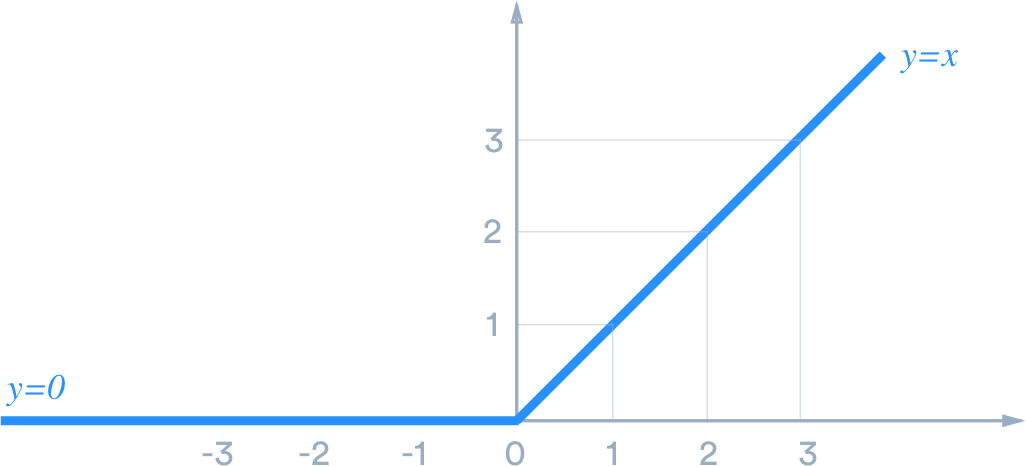
\includegraphics[width=0.5\linewidth]{graphics//chapter3/relu.png}
            \caption{Rectified Linear Unit Activation Function (ReLU) }
            \label{fig:relu}
        \end{figure}
        
        It effectively removes negative values from an activation map by setting them to zero.
        Rectified Linear Unit (ReLU) or rectifier activation function introduces the property of nonlinearity to a deep learning model and solves the vanishing gradients issue. It interprets the positive part of its argument\cite{relu-0}.\par \vspace{1em}
        
    \subsection{Backpropagation in CNN}
    Backpropagation is a process involved in training a neural network. It takes the error rate of a forward propagation and feeds this loss backward through the neural network layers to adjust the weights. It is the practice of fine-tuning the weights of a neural net based on the error rate (i.e. loss) obtained in the previous epoch (i.e. iteration.) Proper tuning of the weights ensures lower error rates, making the model reliable by increasing its generalization.

\section{Transfer Learning and Fine Tuning}

\subsection{Transfer Learning}
It is a technique in which knowledge learned from a  related task is re-used to boost the perfomance on a related task.\cite{tf} It is mainly used when the data available for training is very small.
Specifically, in ConvNet network, many image features such as lines, edges (seen in almost every image) are common to a diffrent image datasets. So, we don't, need to really train our model from scratch as we can used this pre-learned features on our new datasets. That is why large CNN models are rarely trained completely from scratch as large quality labelled datasets and heavy computational resources are hard to find and expensive.\par\vspace{1em}
For eg: in image classification  tasks, knowledge gained from learning to recognize car can be used in recognizing trucks.\par\vspace{1em}
------------------------------------------------------------------------------------------

\subsection{Fine Tuning}
It is an approach to transfer learning in which the parameter of a pretrained model are trained on  a new datasets\cite{ft}. Fine tuning can be done on the entire neural network layer or a subset of the layers, in this case, the layers that are not selected for fine tuning, have their weights frozen during back-propagation (i.e. these weights are not trained/changed) during fine tuning process). A model can also be augmented with adapters, which consists of a far fewer params than the original model, and fine-tuned in a parameter efficient way by adjusting the weights of the adapters models only and leaving the other weights frozen\cite{efficient-fine-tuning}. \par\vspace{1em}
For architecture such as large, deep ConvNet models, its common to keep the lower layer frozens (i.e. layers that are closed to the input layers) as they capture low level features like detecting edges, lines, textures, etc. while the upper layers capture high-level features that are more related to the task in which the models is trained on\cite{Visualizing-and-Understanding-Convolutional-Networks}. More detailed visualisation of the feature learned by ConvNet model are present in \autoref{chap:Model Interpretation and Visualisation}
\par\vspace{1em}
Models that are pretrained on large , general corpora are usually fine tuned by reusing the model parameter as starting points and adding task specific layer from scratch. Fine-tuning the full model is common and often yield better results than training from scratch, however they are computationally expensive.\cite{fine-tuned-pretrained-model-1}\cite{fine-tuned-pretrained-model-2} \par\vspace{1em}
\section{Machine Learning Classifier}
Classifier is a type of machine learning algorithm used to assign a class label to a data input. Classifier algorithms are trained using labeled data; in the image recognition example, for instance, the classifier receives training data that labels images. After sufficient training, the classifier then can receive unlabeled images as inputs and will output classification labels for each image.\par \vspace{1em}

% Classifier algorithms employ sophisticated mathematical and statistical methods to generate predictions about the likelihood of a data input being classified in a given way. In the image recognition example, the classifier statistically predicts whether an image is likely to be a car, a truck, or a person, or some other classification that the classifier has been trained to identify.

    \subsection{ConvNet Models}
        
        \subsubsection{VGG16}
        \begin{figure}
            \centering
            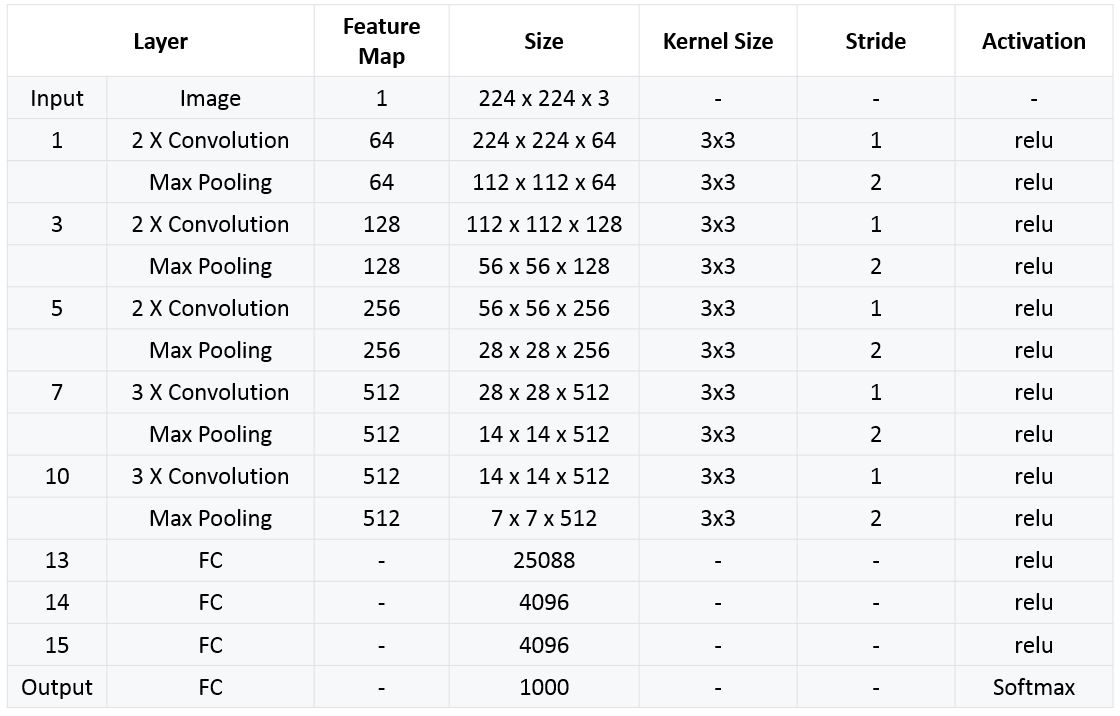
\includegraphics[width=1\linewidth]{graphics//chapter3/vgg16 arch.png}
            \caption{VGG16 Architecture, Source: \cite{WEBSITE:vgg16-arch-diagram}}
            \label{fig:vgg16-arch}
        \end{figure}
        
        VGG16 is a deep convolutional neural network model used for image classification tasks. The network is composed of 16 layers of artificial neurons, which each work to process image information incrementally and improve the accuracy of its predictions.\par \vspace{1em}

        VGG16 uses convolution layers with a 3x3 filter and a stride 1 that are in the same padding and maxpool layer of 2x2 filter of stride 2. It follows this arrangement of convolution and max pool layers consistently throughout the whole architecture. In the end it has two fully connected layers, followed by a softmax for output\cite{vgg16}.\par \vspace{1em} 

        In VGG16, ‘VGG’ refers to the Visual Geometry Group of the University of Oxford, while the ‘16’ refers to the network’s 16 layers that have weights.
        
        \subsubsection{MobileNetV2}
        
        \begin{figure}[h]
            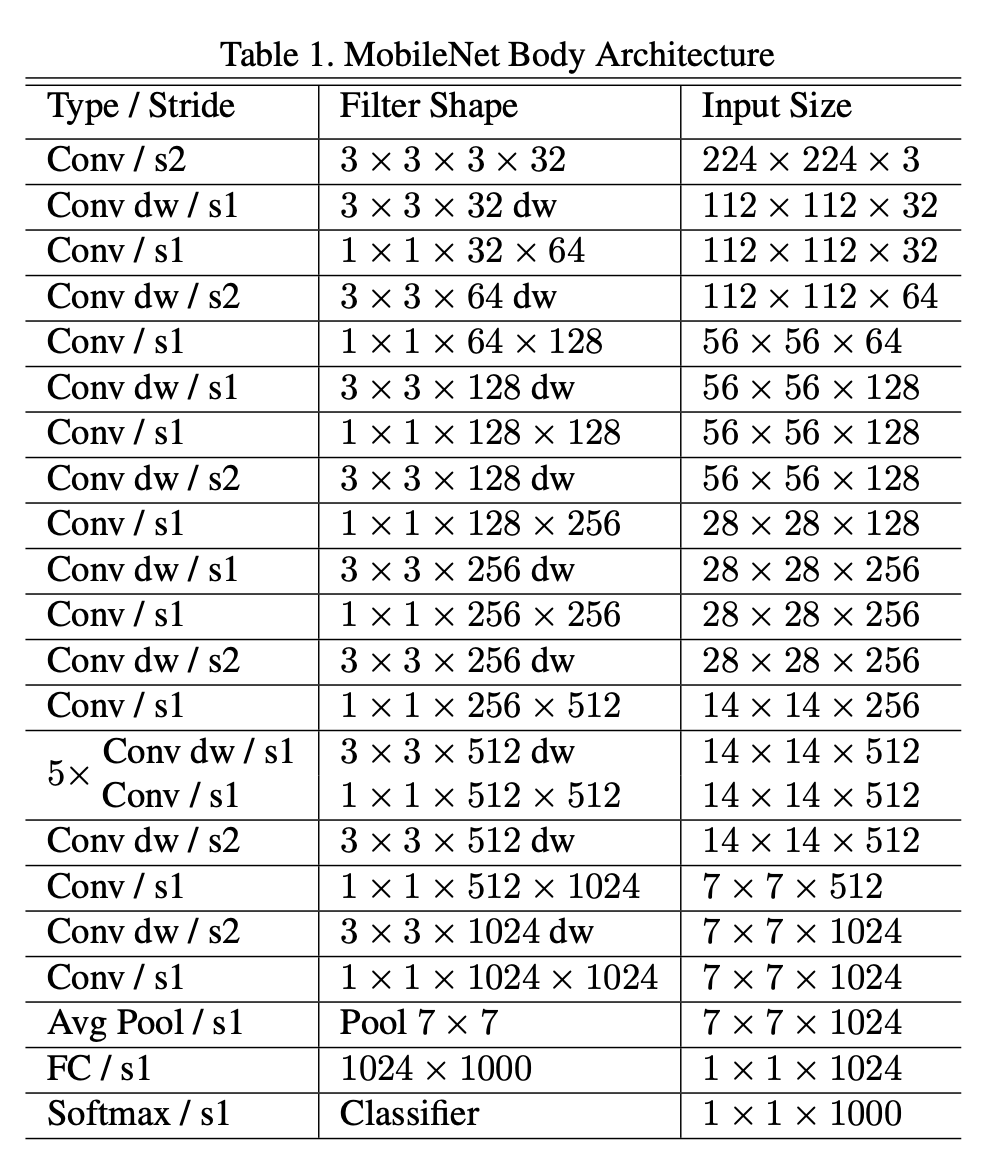
\includegraphics[width=0.5\textwidth, center]{graphics/chapter3/mobnetV1.png}
            \caption{MobileNetV2 Block Diagram, Source: \cite{mobilenetV1}}
            \label{fig:MobileNetV2Block}
        \end{figure}

        \begin{figure}[h]
            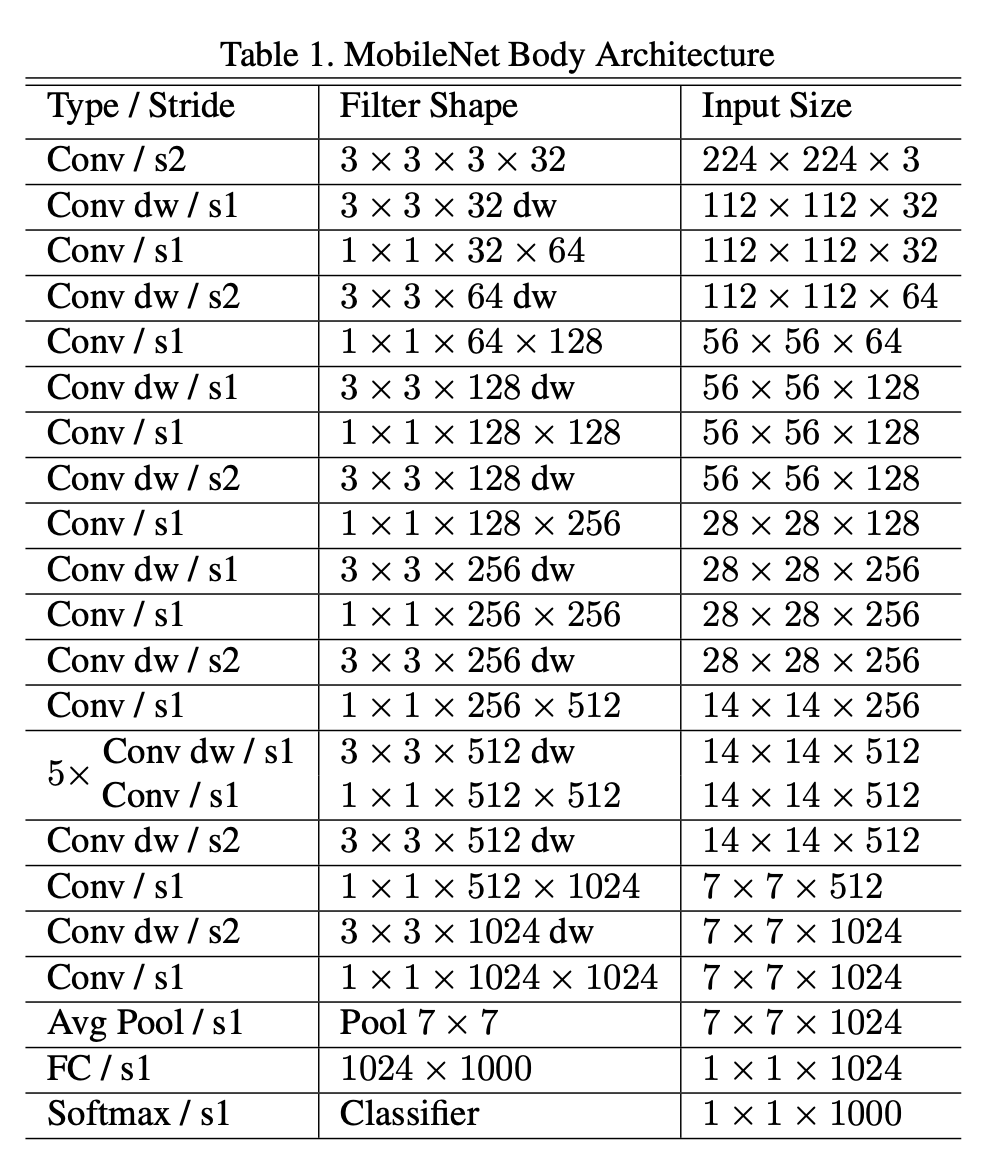
\includegraphics[width=0.5\textwidth, center]{graphics/chapter3/mobnetV1.png}
            \caption{MobileNetV2 Architecture, Source: \cite{mobilenetV1}}
            \label{fig:MobileNetV2}
        \end{figure}
        
        MobileNetV2, is a lightweight convolutional neural network (CNN) architecture, specifically designed for mobile and embedded vision applications. Google researchers developed it as an enhancement over the original MobileNet model. A remarkable aspect of this model is its ability to strike a good balance between model size and accuracy, rendering it ideal for resource-constrained devices \cite{mobilenetV1}.\par \vspace{1em}

        MobileNetV2 architecture incorporates several key features that contribute to its efficiency and effectiveness in image classification tasks. These features include depthwise separable convolution, inverted residuals, bottleneck design, linear bottlenecks, and squeeze-and-excitation (SE) blocks\cite{mobilenetV2}. Each of these features plays a crucial role in reducing the computational complexity of the model while maintaining high accuracy.
        
        \subsubsection{Xception} 
        \begin{figure}
            \centering
            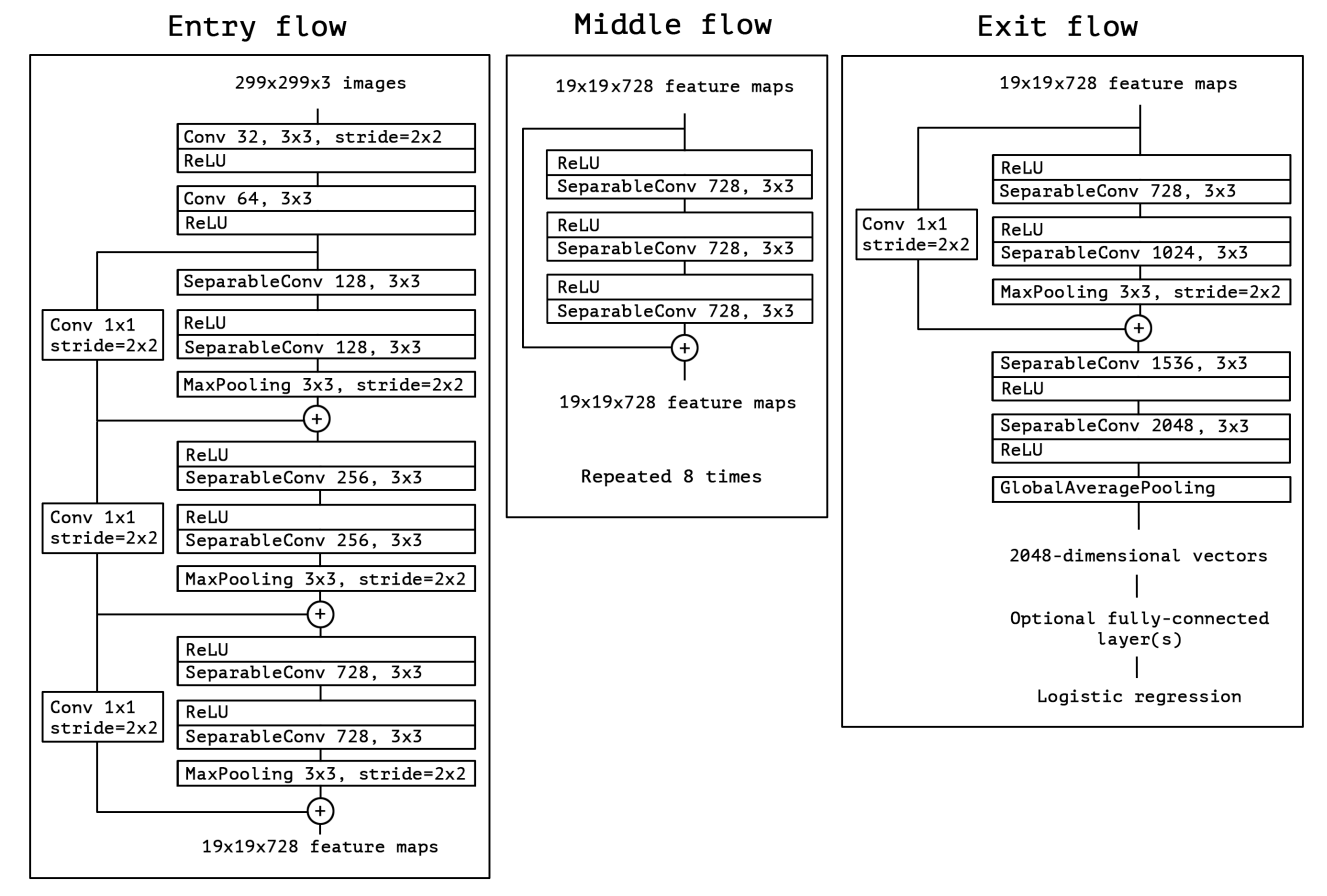
\includegraphics[width=1\linewidth]{graphics//chapter3/xception arch.png}
            \caption{Xception Architecture, Source: \cite{xception}}
            \label{fig:xception-arch}
        \end{figure}
        
        Xception is a deep convolutional neural network architecture that involves Depthwise Separable Convolutions. It was developed by Google researchers. Google presented an interpretation of Inception modules in convolutional neural networks as being an intermediate step in-between regular convolution and the depthwise separable convolution operation (a depthwise convolution followed by a pointwise convolution)\cite{xception}. \par \vspace{1em}
        
        In this light, a depthwise separable convolution can be understood as an Inception module with a maximally large number of towers. This observation leads them to propose a novel deep convolutional neural network architecture inspired by Inception, where Inception modules have been replaced with depthwise separable convolutions.\par \vspace{1em}

        Xception is an efficient architecture that relies on Depthwise Separable Convolution and Shortcuts between Convolution blocks as in ResNet.
        

    \subsection{CNN10L - Scratch Model}
    CNN10L (short 10 Convolutional layer model) is ConvNet Model built by our team.
    It's composed of \textit{10 convolutional layers, 3 max pooling layers, 2 Dense Layers, 1 Global Average 2D Pooling Layers and 1 Dropout Layer}. The Layer architecture is shown in figure \ref{fig:CNN10L}. We used non-linear activation function ReLu in each of the output of convolutional layer. \par\vspace{1em}
    The model is designed in such a way that there is balance in depth and width of feature learned.
    Our aim is to check whether such a shallow model can perform on par with famous very deep convnet model like VGG16, Xception, etc on narrow domain of plant disease detection tasks. Our main emphasis is also to reduce the computational power used by the model by developing a shallow model. And also by training our model from scratch and others by transfer learning, we can check how features learned from larger datasets like \textbf{ImageNet} contribute significantly to improving performance and efficiency when training on narrower domain tasks.
    \par\vspace{1em}
    A detailed description of the model with its input shape and output shape is also given in figure \ref{fig:cnn10l-detail-arch}.\par\vspace{1em}

    \begin{figure}[h]
        \centering
            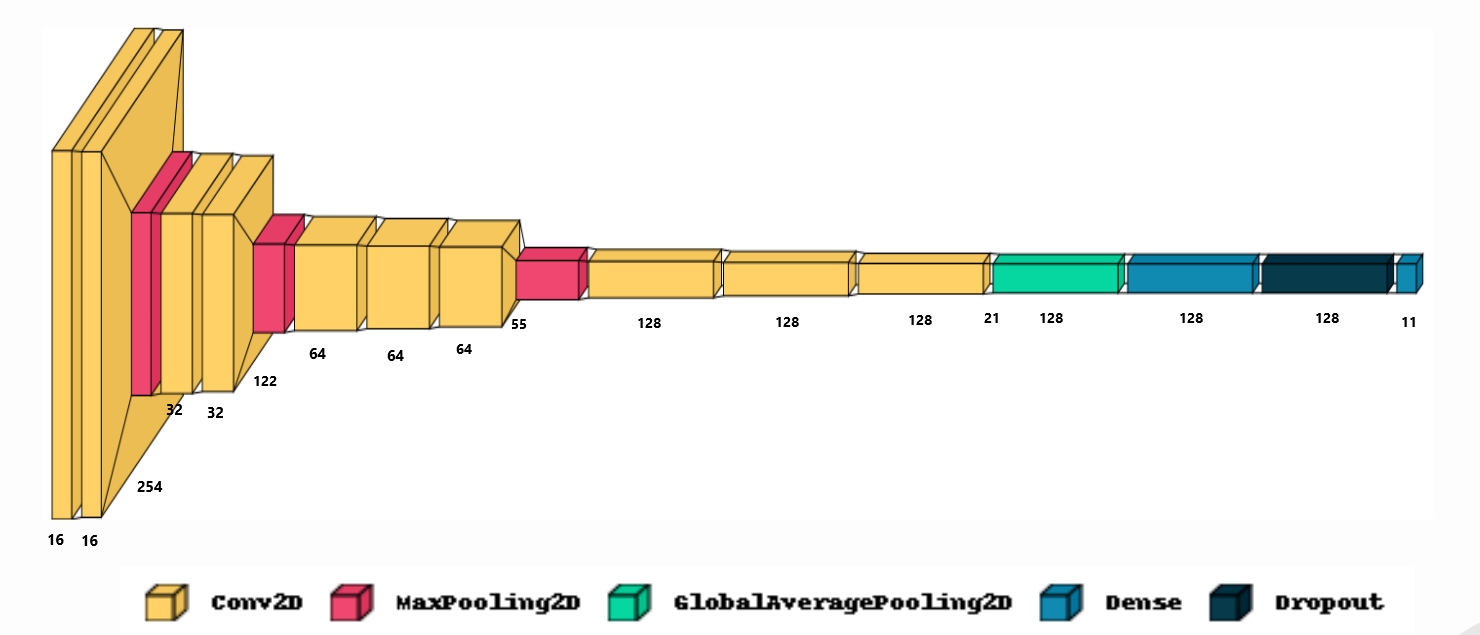
\includegraphics[width=\textwidth]{graphics/chapter3/CNN10L with label.png}
            \caption{CNN10L Architecture}
            \label{fig:CNN10L}
    \end{figure}

    \begin{figure}
        \centering
        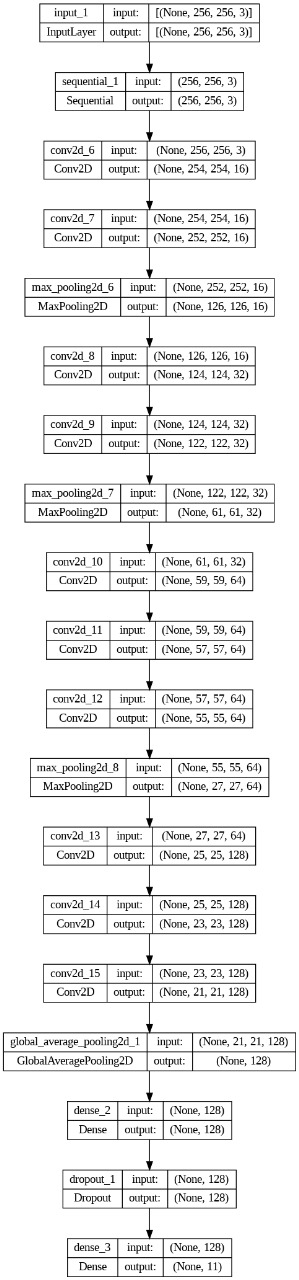
\includegraphics[height=\textheight]{graphics//chapter3/cn10oiedwf.jpg}
        \caption{CNN10L Detail Architecture}
        \label{fig:cnn10l-detail-arch}
    \end{figure}

    \begin{table}[h]
    \centering
    \begin{tabular}{cccc}
        \toprule
        \textbf{Type/Stride} & \textbf{Filter Shape} & \textbf{Input Size} & \textbf{Output Size}\\
        \hline
        \textbf{conv2d / s1} & \textbf{3 x 3 x 16}  & \textbf{3 x 3 x 16} & \textbf{254 x 254 x 3 x 16}\\
        \hline
        \textbf{conv2d / s1} & \textbf{3 x 3 x 16}  & \textbf{254 x 254 x 16} & \textbf{252 x 252 x 16}\\
        \hline
        \textbf{max\_pool / s2} & \textbf{2 x 2}  & \textbf{252 x 252 x 16} & \textbf{126 x 126 x 16}\\
        \hline
        \textbf{conv2d / s1} &\textbf{3 x 3 x 32}  & \textbf{126 x 126 x 16} & \textbf{124 x 124 x 32}\\
        \hline
        \textbf{conv2d / s1} &\textbf{3 x 3 x 32}  & \textbf{124 x 124 x 32} & \textbf{122 x 122 x 32}\\
        \hline
        \textbf{max\_pool / s2} & \textbf{2 x 2}  & \textbf{122 x 122 x 32} & \textbf{61 x 61 x 32}\\
        \hline
        \textbf{conv2d / s1} & \textbf{3 x 3 x 64}  & \textbf{61 x 61 x 32} & \textbf{59 x 59 x 64}\\
        \hline
        \textbf{conv2d / s1} & \textbf{3 x 3 x 64}  & \textbf{59 x 59 x 64} & \textbf{57 x 57 x 64}\\
        \hline
        \textbf{conv2d / s1} & \textbf{3 x 3 x 64} & \textbf{57 x 57 x 64} & \textbf{55 x 55 x 64}\\
        \hline
        \textbf{max\_pool / s2} & \textbf{2 x 2} & \textbf{55 x 55 x 64} & \textbf{27 x 27 x 64}\\
        \hline
        \textbf{conv2d / s1} & \textbf{3 x 3 x 128} & \textbf{27 x 27 x 64} & \textbf{25 x 25 x 128}\\
        \hline
        \textbf{conv2d / s1} & \textbf{3 x 3 x 128} & \textbf{25 x 25 x 128} & \textbf{23 x 23 x 128}\\
        \hline
        \textbf{conv2d / s1} & \textbf{3 x 3 x 128} & \textbf{23 x 23 x 128} & \textbf{21 x 21 x 128}\\
        \hline
        \textbf{global avg pool 2D} & & \textbf{21 x 21 x 128} & \textbf{128}\\
        \hline
        \textbf{FCN} & & \textbf{128} & \textbf{128}\\
        \hline
        \textbf{dropout} & & \textbf{128} & \textbf{128}\\
        \hline
        \textbf{FCN} & & \textbf{128} & \textbf{11}\\

        \bottomrule


    \end{tabular}
    \caption{CNN10L Architecture}
    \label{tab:cnn10L-arch}
\end{table}
    
    \textbf{Key features of CNN10L Model:}
    \begin{enumerate}
        \item \textbf{Multiple Convolution Layers Before Pooling}\\
        \textbf{Feature Extraction:} By stacking multiple convolutional layers before each pooling layer, the model can capture more detailed and abstract features at each stage. This allows for a richer and more complex feature representation.

        \item \textbf{Hierarchical Feature Learning}\\
        \textbf{Layered Learning:} Early layers focus on simple features like edges, while deeper layers capture more complex patterns such as shapes and textures. This hierarchical approach enables the network to learn a comprehensive representation of the input data.
        
        \item \textbf{Reduced Spatial Dimensions}\\
        \textbf{Pooling Benefits:} The max pooling layers help in reducing the spatial dimensions of the feature maps, decreasing computational load and preventing overfitting. This leads to a more efficient and effective model.
        
        \item \textbf{Receptive Field Expansion}\\
        \textbf{Context Awareness:} Each pooling operation increases the receptive field of the subsequent layers, allowing them to incorporate more context from the input image. This helps in detecting more abstract and spatially extended features.
        
        \item \textbf{Non Linearity and Expressive Power}\\
        \textbf{Activation Functions:} Convolutional layers typically include non-linear activation functions (e.g., ReLU). Stacking multiple convolutions increases the model's expressive power, enabling it to capture complex relationships in the data.
        
    \end{enumerate}\par\vspace{1em}

    The reasons, why we build our model in this form are described as follows: \\
    \begin{itemize}
        \item \textbf{Enhanced Feature Learning}\\
        By having multiple convolutional layers before pooling, the model can learn more complex and detailed features, which are crucial for high performance in tasks like image classification.
        
        \item \textbf{Balanced Computational Efficiency}\\
        The architecture balances the depth and width of the network, ensuring that it can handle complex features without becoming too computationally expensive.
        
        \item \textbf{Improved Performance}\\
        imilar architectures, such as VGGNet, have shown high performance in various image classification benchmarks. The design choices are often guided by empirical validation and successful practices in the field.
        
        \item \textbf{Prevention of Overfitting}\\
        Periodic max pooling reduces the number of parameters and helps prevent overfitting, which is particularly important for deeper networks.
        
    \end{itemize}
    

    
    \subsection{Traditional/Classical Machine Learning Classifier Model}
    
        \subsubsection{Support Vector Machine}
        Support Vector Machine or SVM is one of the most popular Supervised Learning algorithms, which is used for Classification as well as Regression problems. The goal of the SVM algorithm is to create the best line or decision boundary that can segregate n-dimensional space into classes so that we can easily put the new data point in the correct category in the future. This best decision boundary is called a hyperplane\cite{svm-0}\cite{kernel}.\par \vspace{1em}

        \begin{figure}
            \centering
            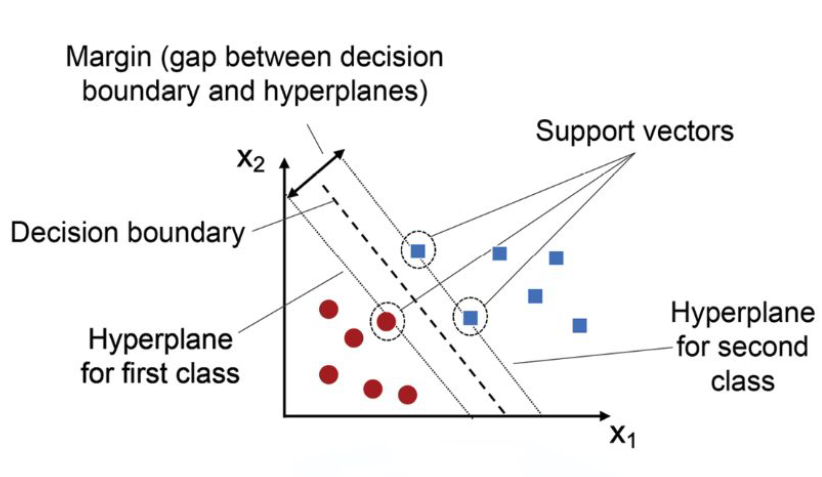
\includegraphics[width=0.75\linewidth]{graphics//chapter3/svm linear.png}
            \caption{SVM in linearly separable class, Source:\cite{gml}}
            \label{fig:svm-linear}
        \end{figure}

        \begin{figure}
            \centering
            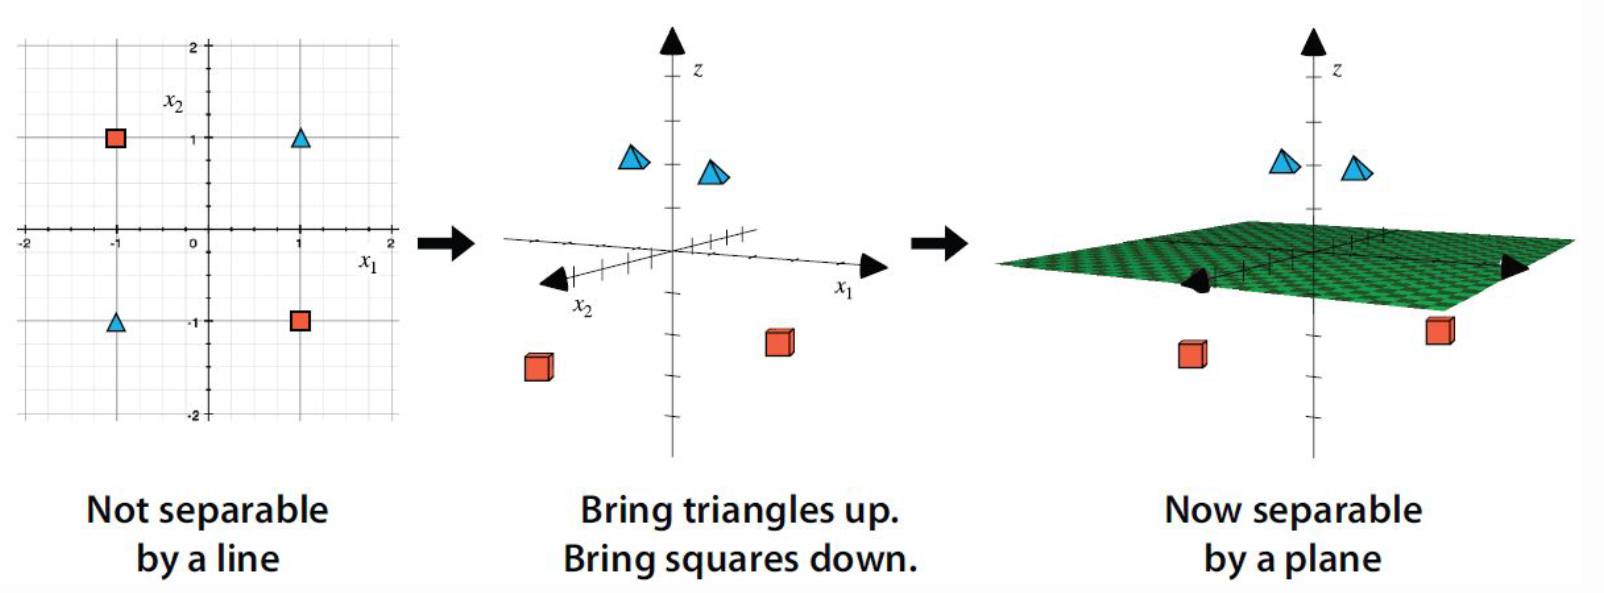
\includegraphics[width=1\linewidth]{graphics//chapter3/svm non linear.png}
            \caption{SVM using Kernel Trick to classify non-linearly separable classes, Source: \cite{gml}}
            \label{fig:svm-nonlinear}
        \end{figure}
        
        SVM chooses the extreme points/vectors that help in creating the hyperplane. These extreme cases are called as support vectors, and hence algorithm is termed as Support Vector Machine.
        
        \subsubsection{K-Nearest Neighbor (KNN)}
        The k-nearest neighbors (KNN) algorithm is a non-parametric, supervised learning classifier, which uses proximity to make classifications or predictions about the grouping of an individual data point. While the KNN algorithm can be used for either regression or classification problems, it is typically used as a classification algorithm, working off the assumption that similar points can be found near one another\cite{knn}.\par \vspace{1em}

        \begin{figure}
            \centering
            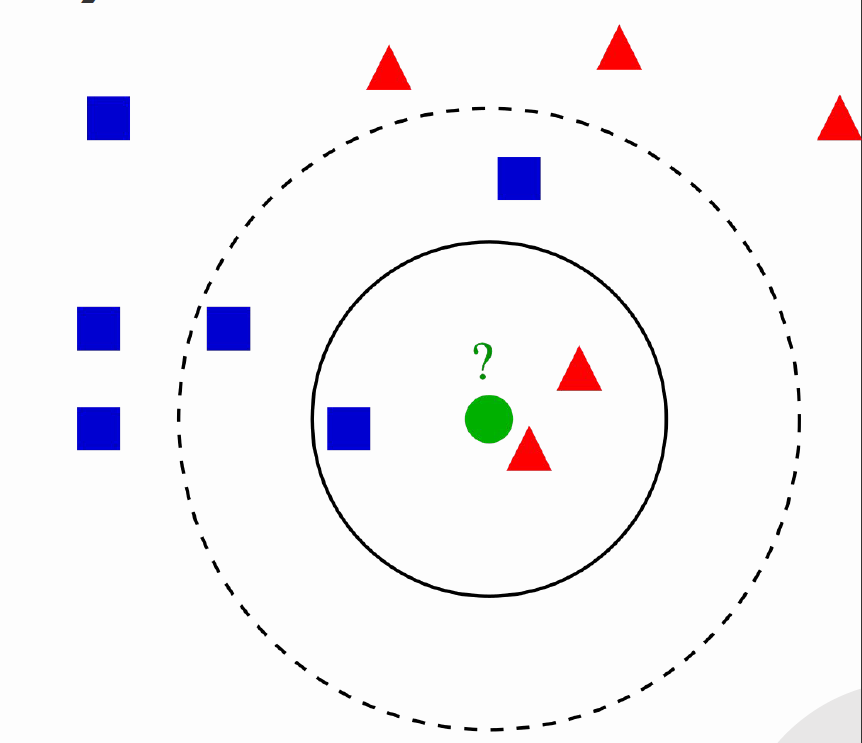
\includegraphics[width=0.75\linewidth]{graphics//chapter3/knn.png}
            \caption[Example of k-NN classification]{Example of k-NN classification. \\The test sample (green dot) should be classified either to blue squares or to red triangles. If k = 3 (solid line circle) it is assigned to the red triangles because there are 2 triangles and only 1 square inside the inner circle. If k = 5 (dashed line circle) it is assigned to the blue squares (3 squares vs. 2 triangles inside the outer circle)\cite{knn-credit}.}
            \label{fig:knn}
        \end{figure}
        
        For classification problems, a class label is assigned on the basis of a majority vote—i.e. the label that is most frequently represented around a given data point is used.
        
        \subsubsection{Ensemble Techniques}
        Ensemble methods use multiple learning algorithms to obtain better predictive performance than could be obtained from any of the constituent learning algorithms alone\cite{em}.\par\vspace{1em}
        
        Supervised learning algorithms perform the task of searching through a hypothesis space to find a suitable hypothesis that will make good predictions with a particular problem. Even if the hypothesis space contains hypotheses that are very well-suited for a particular problem, it may be very difficult to find a good one. Ensembles combine multiple hypotheses to form a (hopefully) better hypothesis. \par\vspace{1em}
        
        Ensemble learning trains two or more Machine Learning algorithms to a specific classification or regression task. The algorithms within the ensemble learning model are generally referred as “base models”, “base learners” or “weak learners” in literature. The base models can be constructed using a single modelling algorithm or several different algorithms. The idea is train a diverse collection of weak performing models to the same modelling task. As a result, the predicted or classified outcomes of each weak learner have poor predictive ability (high bias, i.e. high model errors) and among the collection of all weak learners the outcome and error values exhibit high variance. Fundamentally, an ensemble learning model trains many (at least 2) high-bias (weak) and high-variance (diverse) models to be combined into a stronger and better performing model. Essentially, it’s a set of algorithmic models — which would not produce satisfactory predictive results individually — that get’s combined or averaged over all base models to produce a single high performing, accurate and low-variance model to fit the task as required.\par\vspace{1em}
        
        Ensemble learning typically refers to Bagging (bootstrap-aggregating), Boosting or Stacking/Blending techniques to induce high variability among the base models. Bagging creates diversity by generating random samples from the training observations and fitting the same model to each different sample — also known as “homogeneous parallel ensembles”. Boosting follows an iterative process by sequentially training each next base model on the up-weighted errors of the previous base model’s errors, producing an additive model to reduce the final model errors — also known as “sequential ensemble learning”. Stacking or Blending consists of different base models, each trained independently (i.e. diverse/high variability) to be combined into the ensemble model — producing a “heterogeneous parallel ensemble”. Common applications of ensemble learning include Random Forests (extension of Baggin), Boosted Tree-Models, Gradient Boosted Tree-Models and models in applications of stacking are generally more task-specific — such as combing clustering techniques with other parametric and/or non-parametric techniques. \par\vspace{1em}
        
        \subsubsection{Random Forest}
        
        Random forests or random decision forests is an ensemble learning method for classification, regression and other tasks that operates by constructing a multitude of decision trees at training time. For classification tasks, the output of the random forest is the class selected by most trees. For regression tasks, the mean or average prediction of the individual trees is returned. Random decision forests correct for decision trees' habit of overfitting to their training set.\par\vspace{1em}
        
        \begin{figure}
            \centering
            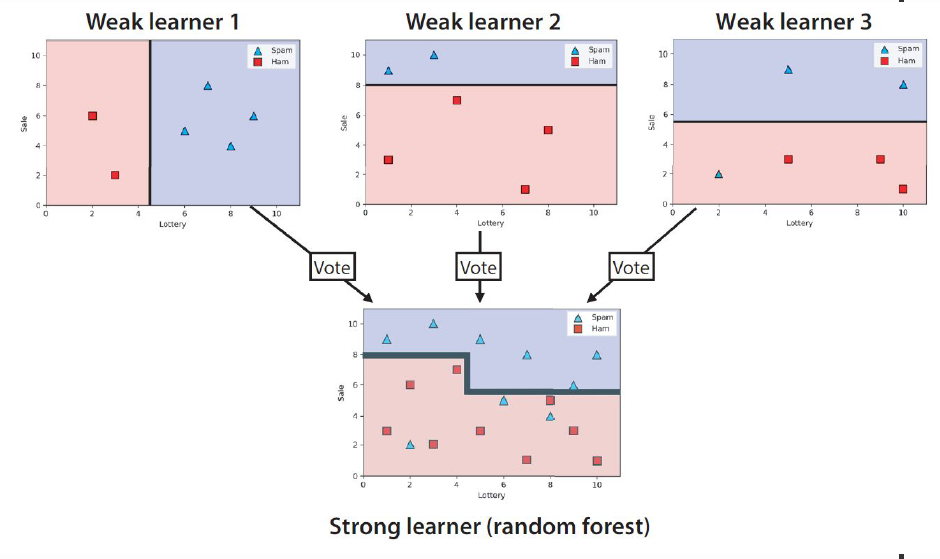
\includegraphics[width=1\linewidth]{graphics//chapter3/random forest.png}
            \caption{Random Forest, Source: \cite{gml}}
            \label{fig:random-forest}
        \end{figure}
        
         Trees that are grown very deep tend to learn highly irregular patterns: they overfit their training sets, i.e. have low bias, but very high variance. Random forests are a way of averaging multiple deep decision trees, trained on different parts of the same training set, with the goal of reducing the variance. This comes at the expense of a small increase in the bias and some loss of interpretability, but generally greatly boosts the performance in the final model\cite{rf-1}\cite{rf-2}.\par\vspace{1em}
        
        \subsubsection{Extreme Gradient Boosting (XGBoost)}   

        \begin{figure}
            \centering
            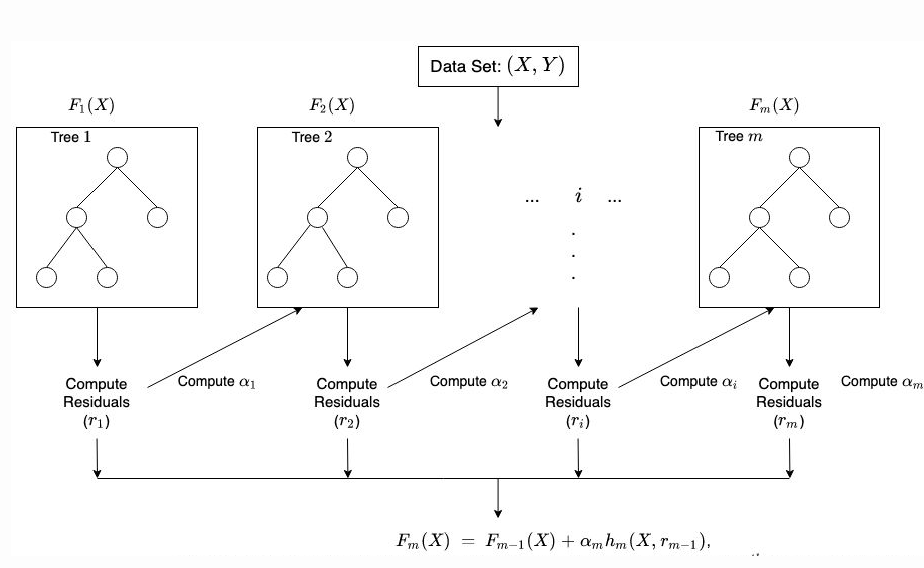
\includegraphics[width=1\linewidth]{graphics//chapter3/xgboost-tree.png}
            \caption{XGBoost Tree, Source: \cite{WEBSITE:xgb-credit-0}}
            \label{fig:xgboost-tree}
        \end{figure}
        
        XGBoost (eXtreme Gradient Boosting) is an advanced implementation of gradient boosting algorithm. It’s a powerful machine learning algorithm especially popular for structured or tabular data. XGBoost has gained fame for its performance in a wide range of machine learning competitions and tasks\cite{xgb}.\par\vspace{1em}
        Since its introduction, this algorithm has not only been credited with winning numerous Kaggle competitions but also for being the driving force under the hood for several cutting-edge industry applications. \par\vspace{1em}
        
        \begin{figure}
            \centering
            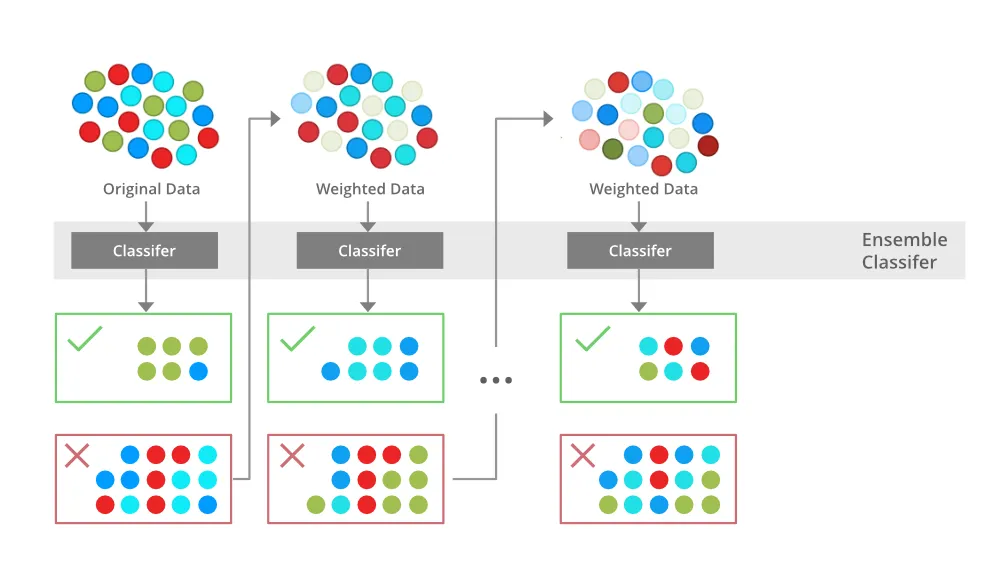
\includegraphics[width=\linewidth]{graphics//chapter3/xgboost1.png}
            \caption{XGBoost Working, Source:\cite{WEBSITE:xgb-credit-1}}
            \label{fig:xgboost-1}
        \end{figure}        

        \textbf{XGBoost Features: }
        \begin{enumerate}
            \item \textbf{Parallelization:} XGBoost approaches the process of sequential tree building using parallelized implementation. This is possible due to the interchangeable nature of loops used for building base learners; the outer loop that enumerates the leaf nodes of a tree, and the second inner loop that calculates the features. This nesting of loops limits parallelization because without completing the inner loop (more computationally demanding of the two), the outer loop cannot be started. Therefore, to improve run time, the order of loops is interchanged using initialization through a global scan of all instances and sorting using parallel threads. This switch improves algorithmic performance by offsetting any parallelization overheads in computation.
            \item \textbf{Tree Pruning:} The stopping criterion for tree splitting within GBM framework is greedy in nature and depends on the negative loss criterion at the point of split. XGBoost uses ‘max\_depth’ parameter as specified instead of criterion first, and starts pruning trees backward. This ‘depth-first’ approach improves computational performance significantly.
            \item \textbf{Hardware Optimization:} This algorithm has been designed to make efficient use of hardware resources. This is accomplished by cache awareness by allocating internal buffers in each thread to store gradient statistics. Further enhancements such as ‘out-of-core’ computing optimize available disk space while handling big data-frames that do not fit into memory.
        \end{enumerate}

        \textbf{Algorithmic Enhancements:}
        \begin{enumerate}
            \item \textbf{Regularization:} It penalizes more complex models through both LASSO (L1) and Ridge (L2) regularization to prevent overfitting.
            \item \textbf{Sparsity Awareness:} XGBoost naturally admits sparse features for inputs by automatically ‘learning’ best missing value depending on training loss and handles different types of sparsity patterns in the data more efficiently.
            \item \textbf{Weighted Quantile Sketch:} XGBoost employs the distributed weighted Quantile Sketch algorithm to effectively find the optimal split points among weighted datasets.
            \item \textbf{Cross-validation:} The algorithm comes with built-in cross-validation method at each iteration, taking away the need to explicitly program this search and to specify the exact number of boosting iterations required in a single run.
        \end{enumerate}

\newpage
% \section{Loss Function}
% A loss function or cost function (sometimes also called an error function) is a function that maps an event or values of one or more variables onto a real number intuitively representing some "cost" associated with the event. An optimization problem seeks to minimize a loss function. An objective function is either a loss function or its opposite (in specific domains, variously called a reward function, a profit function, a utility function, a fitness function, etc.), in which case it is to be maximized. The loss function could include terms from several levels of the hierarchy.
% \par \vspace{1em}

% \begin{figure}
%     \centering
%     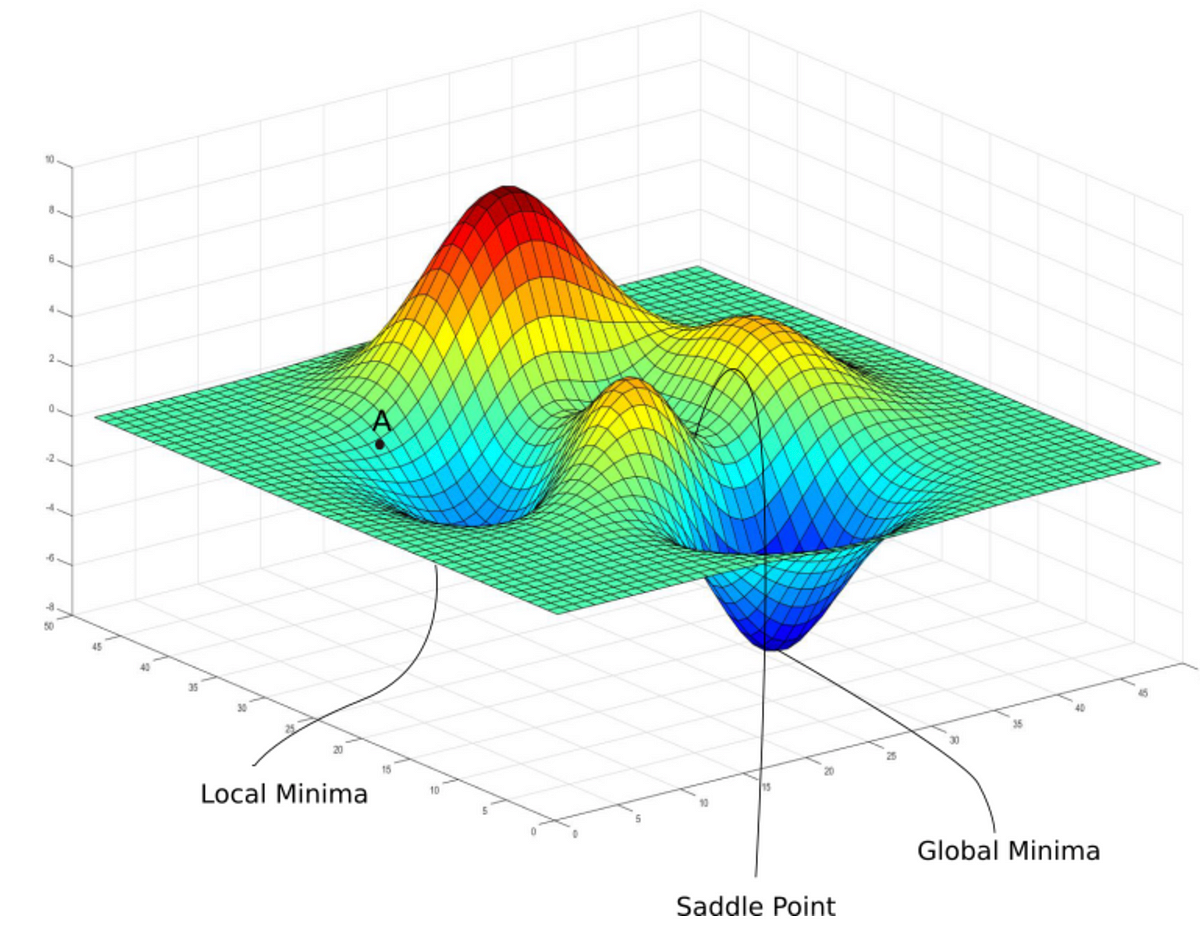
\includegraphics[width=0.75\linewidth]{graphics//chapter3/loss with local global minima.png}
%     \caption{Loss Function with a local, global and saddle point}
%     \label{fig:loss-lgs}
% \end{figure}

% \begin{figure}
%     \centering
%     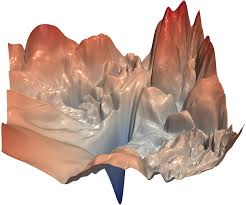
\includegraphics[width=0.75\linewidth]{graphics//chapter3/loss landscape.png}
%     \caption{Loss surface learned by neural networks }
%     \label{fig:loss-landscape}
% \end{figure}

% In statistics, typically a loss function is used for parameter estimation, and the event in question is some function of the difference between estimated and true values for an instance of data. The concept, as old as Laplace, was reintroduced in statistics by Abraham Wald in the middle of the 20th century.In the context of economics, for example, this is usually economic cost or regret. In classification, it is the penalty for an incorrect classification of an example. In actuarial science, it is used in an insurance context to model benefits paid over premiums, particularly since the works of Harald Cramér in the 1920s.In optimal control, the loss is the penalty for failing to achieve a desired value. In financial risk management, the function is mapped to a monetary loss.
%     \subsection{Mean Squared Error (MSE)}
%     The mean squared error (MSE) or mean squared deviation (MSD) of an estimator (of a procedure for estimating an unobserved quantity) measures the average of the squares of the errors i.e., the average squared difference between the estimated values and the actual value. MSE is a risk function, corresponding to the expected value of the squared error loss.The fact that MSE is almost always strictly positive (and not zero) is because of randomness or because the estimator does not account for information that could produce a more accurate estimate.In machine learning, specifically empirical risk minimization, MSE may refer to the empirical risk (the average loss on an observed data set), as an estimate of the true MSE (the true risk: the average loss on the actual population distribution).\par\vspace{1em}
%  % \newpage
%  The MSE either assesses the quality of a predictor (i.e., a function mapping arbitrary inputs to a sample of values of some random variable), or of an estimator (i.e., a mathematical function mapping a sample of data to an estimate of a parameter of the population from which the data is sampled). In the context of prediction, understanding the prediction interval can also be useful as it provides a range within which a future observation will fall, with a certain probability. The definition of an MSE differs according to whether one is describing a predictor or an estimator.\par\vspace{1em}

% If a vector of \(\displaystyle{n}\) predictions is generated from a sample of \(\displaystyle{n}\) data points on all variables, and \(\displaystyle{y}\) is the vector of observed values of the variable being predicted, with 
% \(\displaystyle {\hat {y}}\) being the predicted values, then the within-sample MSE of the predictor is computed as:
% \begin{center}
%     \(\text{MSE} = \frac{1}{n} \sum_{i=1}^{n} (y_i - \hat{y}_i)^2\)
% \end{center}
 
%     \subsection{Cross Entropy Loss}
%     Cross-Entropy Loss is also known as logarithmic loss, log loss or logistic loss. Each probability of the predicted class is compared with the actual class and loss is calculated which penalizes the probability based on how far it is from the actual expected value. The penalty is logarithmic in nature yielding a large score for large differences close to 1 and small score for small differences tending to 0. A perfect model has a cross-entropy loss of 0.
% \par \vspace{1em}
% Cross-entropy is defined as:
%         \begin{center}
%             \( L_{CE} = - \sum_{i=1}^{n} t_{i} log(p_{i}) \), for n classes     
%         \end{center}
   
      
    
% \section{Optimizer}
% Optimizers are algorithms that dynamically fine-tune a model’s parameters throughout the training process, aiming to minimize a predefined loss function. These specialized algorithms facilitate the learning process of neural networks by iteratively refining the weights and biases based on the feedback received from the data. 
%     \subsection{Adam}
%     Adam optimizer, short for “Adaptive Moment Estimation,” is an iterative optimization algorithm used to minimize the loss function during the training of neural networks. It can be looked at as a combination of RMSprop and Stochastic Gradient Descent with momentum.\par \vspace{1em}
    
%     It uses the squared gradients to scale the learning rate like RMSprop, and it takes advantage of momentum by using the moving average of the gradient instead of the gradient itself, like SGD with momentum. This combines Dynamic Learning Rate and Smoothening to reach the global minima.
    
%     \subsection{RMS Prop}
%     RMSProp (Root Mean Squared Propagation) is an adaptive learning rate optimization algorithm. It is an extension of the popular Adaptive Gradient Algorithm and is designed to dramatically reduce the amount of computational effort used in training neural networks. This algorithm works by exponentially decaying the learning rate every time the squared gradient is less than a certain threshold. This helps reduce the learning rate more quickly when the gradients become small. In this way, RMSProp is able to smoothly adjust the learning rate for each of the parameters in the network, providing a better performance than regular Gradient Descent alone.
    
% \section{Exploding and Vanishing Gradient}
% \subsection{Exploding Gradient}
% Exploding Gradients Problem often comes up, as backpropagation algorithm advances downwards(or backward) from the output layer towards the input layer. The gradients often get larger and larger. This causes very large weight updates and causes the gradient descent to diverge.
% \subsection{Vanishing Gradient}
% Vanishing Gradients Problem often comes up, as backpropagation algorithm advances downwards(or backward) from the output layer towards the input layer. The gradients often get smaller and smaller and approach zero which eventually leaves the weights of the initial or lower layers nearly unchanged. As a result, the gradient descent never converges to the optimum.

\section{K Fold Validation}
K-fold cross validation is a powerful technique for evaluating predictive models. It involves splitting the dataset into k subsets or folds, where each fold is used as the validation set in turn while the remaining k-1 folds are used for training. This process is repeated k times, and performance metrics such as accuracy, precision, and recall are computed for each fold. By averaging these metrics, we obtain an estimate of the model’s generalization performance. This method is essential for model assessment, selection, and hyperparameter tuning, offering a reliable measure of a model’s effectiveness. Compared to leave-one-out cross-validation, which uses k equal to the number of samples, K-fold cross-validation is computationally efficient and widely used in practice\cite{esl}\cite{kfold-1}.\par \vspace{1em}
\begin{figure}
    \centering
    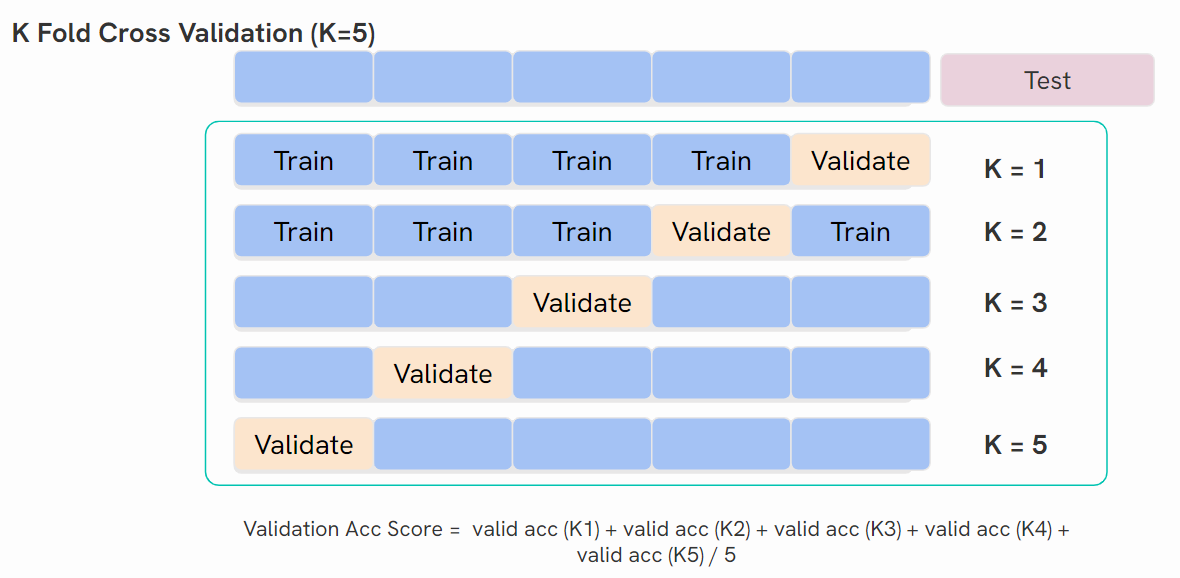
\includegraphics[width=1\linewidth]{graphics//chapter3/k fold.png}
    \caption{K Fold Cross Validation}
    \label{fig:k-fold}
\end{figure}

In each set (fold) training and the test would be performed precisely once during this entire process. It helps us to avoid overfitting. As we know when a model is trained using all of the data in a single short and give the best performance accuracy. To resist this k fold cross validation in machine learning cross-validation helps us to build the model is a generalized one.

    \subsection{Stratified K fold validation}
    Stratified K-Fold Cross-Validation is a variation of K-Fold Cross-Validation that ensures each fold maintains the same proportion of observations for each target class as the complete dataset. This is especially crucial for datasets where one class might be heavily underrepresented.

    \begin{figure}
        \centering
        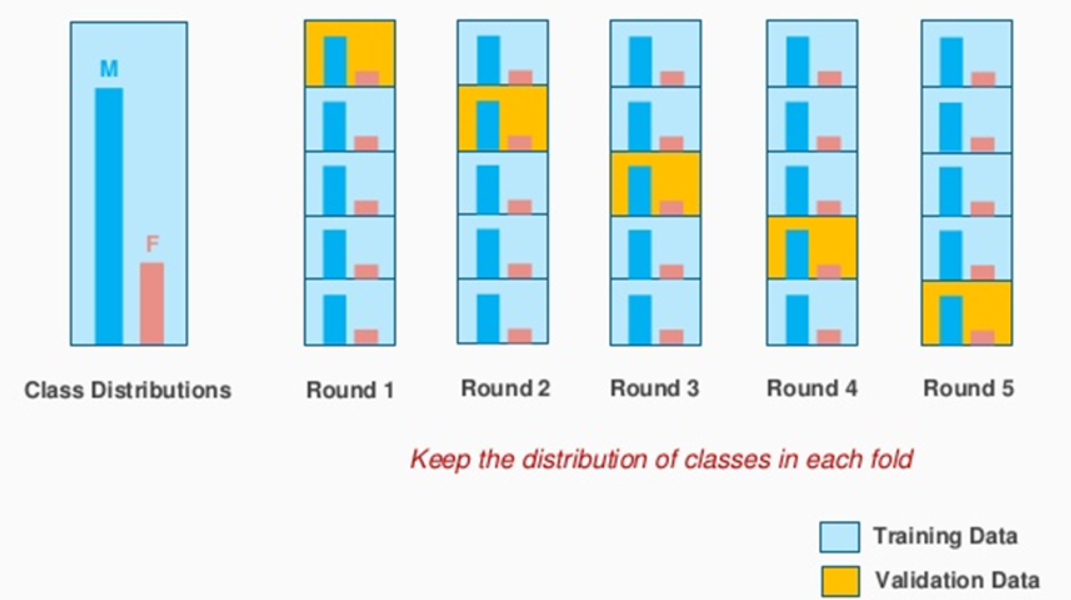
\includegraphics[width=0.75\linewidth]{graphics//chapter3/stratified k fold.png}
        \caption{Stratified K Fold Validation, Source: \cite{WEBSITE:skfold-credit}}
        \label{fig:stratified-k-fold}
    \end{figure}
    
% \section{Hyperparameter Tuning}
% Hyperparameter tuning is the process of selecting the optimal values for a machine learning model’s hyperparameters. Hyperparameters are settings that control the learning process of the model, such as the learning rate, the number of neurons in a neural network, or the kernel size in a support vector machine. The goal of hyperparameter tuning is to find the values that lead to the best performance on a given task.
%     \subsection{Grid Search}
%     \begin{figure}
%         \centering
%         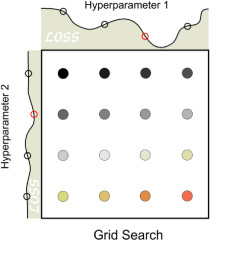
\includegraphics[width=0.5\linewidth]{graphics//chapter3/grid search.png}
%         \caption{Grid Search}
%         \label{fig:grid-search}
%     \end{figure}
%     Grid search fits the model using all possible combinations after creating a grid of potential discrete hyperparameter values. Each set's model performance is then logged and then a combination that produces the best results is chosen. This approach is called GridSearchCV, because it searches for the best set of hyperparameters from a grid of hyperparameters values. 

% \section{Batch Normalisation}
% Batch normalization is a method used to make training of artificial neural networks faster and more stable through normalization of the layers' inputs by re-centering and re-scaling.
% While the effect of batch normalization is evident, the reasons behind its effectiveness remain under discussion. It was believed that it can mitigate the problem of internal covariate shift, where parameter initialization and changes in the distribution of the inputs of each layer affect the learning rate of the network.

% \begin{figure}
%     \centering
%     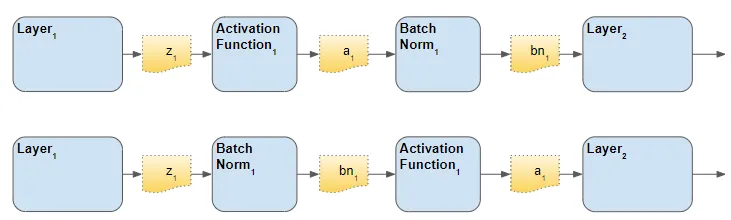
\includegraphics[width=1\linewidth]{graphics//chapter3/batch norm.png}
%     \caption{Batch Normalisation used in Neural Network Model}
%     \label{fig:batch-norm}
% \end{figure}

% \section{Dropout in Neural Network}
% Dropout is a technique used in neural networks to improve model performance and reduce overfitting. It works by randomly "dropping out" (setting to zero) a certain percentage of input and hidden units during the training process. By doing so, it helps the model generalize better and reduces the reliance on specific units, making the model more robust and less likely to overfit the training data.
% \par \vspace{1em}
% \begin{figure}
%     \centering
%     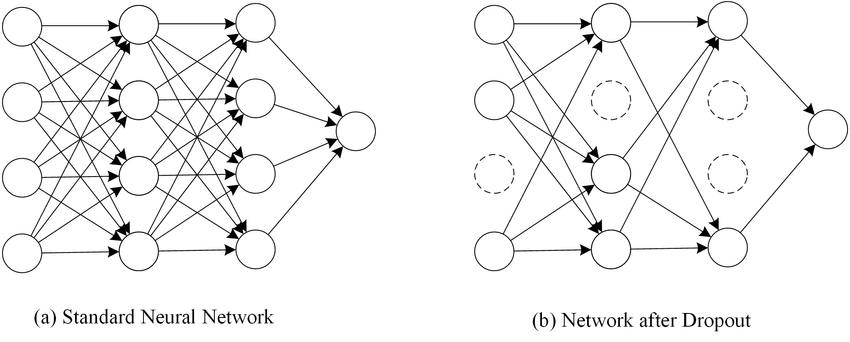
\includegraphics[width=1\linewidth]{graphics//chapter3/dropout.png}
%     \caption{Dropout}
%     \label{fig:dropout}
% \end{figure}
% During each training iteration, dropout randomly selects a fraction of the input and hidden units to be "dropped out" or set to zero. The fraction of units to be dropped out is a hyperparameter that can be tuned. This process helps prevent the neural network from relying too heavily on specific units and encourages the network to learn more robust and general features. Dropout effectively creates an ensemble of multiple subnetworks that share parameters, leading to improved generalization and reducing the risk of overfitting.
% \par \vspace{1em}
% Dropout is important because it helps address the overfitting problem in neural networks. Overfitting occurs when the model performs well on the training data but fails to generalize to unseen data. By randomly dropping out units, dropout forces the network to learn more redundant representations and prevents it from relying too heavily on specific units. This regularization technique improves the network's ability to generalize and perform well on unseen data.

% \newpage
\section{Perfomance Metrics for Image Classification}
Evaluating the performance of a Machine learning model is one of the important steps while building an effective ML model. To evaluate the performance or quality of the model, different metrics are used, and these metrics are known as performance metrics or evaluation metrics. These performance metrics help us understand how well our model has performed for the given data. In this way, we can improve the model's performance by tuning the hyper-parameters. Each ML model aims to generalize well on unseen/new data, and performance metrics help determine how well the model generalizes on the new dataset\cite{c-eval}.
\par \vspace{1em}
In a classification problem, the category or classes of data is identified based on training data. The model learns from the given dataset and then classifies the new data into classes or groups based on the training. It predicts class labels as the output, such as Yes or No, 0 or 1, Spam or Not Spam, etc. \par \vspace{1em}

To evaluate the performance of a classification model, different metrics are used, and some of them are as follows:

    \subsection{Accuracy}
    The accuracy metric is one of the simplest Classification metrics to implement, and it can be determined as the number of correct predictions to the total number of predictions.

    \begin{center}
        \(\displaystyle{Accuracy = \frac{\text{No Of Correct Prediction}}{\text{Total Number Of Prediction}}}\) 
    \end{center}


    \subsection{Confusion Matrix}
    A confusion matrix is a tabular representation of prediction outcomes of any binary classifier, which is used to describe the performance of the classification model on a set of test data when true values are known.

    \begin{figure}
        \centering
        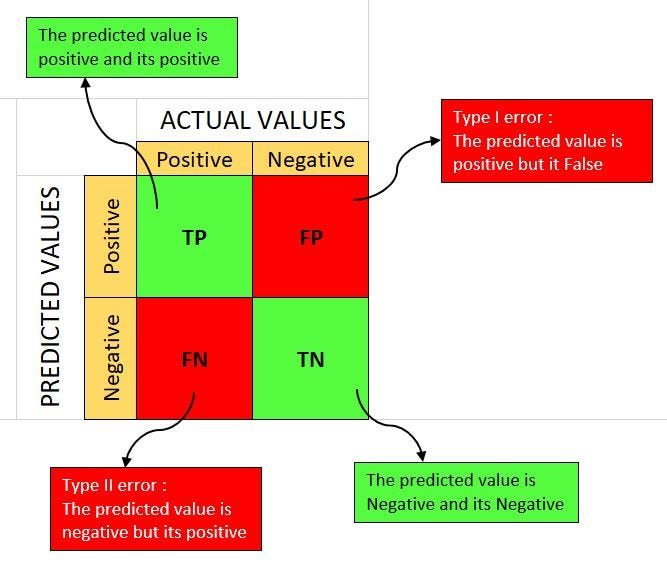
\includegraphics[width=0.75\linewidth]{graphics//chapter3/typical confusion matrix.png}
        \caption{Confusion Matrix, Source: \cite{WEBSITE:cm-credit}}
        \label{fig:typical-confusion-matrix}
    \end{figure}

    In general, the confusion matrix table is divided into four terminologies, which are as follows:
    \begin{enumerate}
        \item \textbf{True Positive(TP):} In this case, the prediction outcome is true, and it is true in reality, also.
        \item \textbf{True Negative(TN):} in this case, the prediction outcome is false, and it is false in reality, also.
        \item \textbf{False Positive(FP):} In this case, prediction outcomes are true, but they are false in actuality.
        \item \textbf{False Negative(FN):} In this case, predictions are false, and they are true in actuality.
    \end{enumerate}



    
    \subsection{Precision}    
    Precision (also called positive predictive value) gives the proportion of positive identifications that were actually correct. Written as a formula\cite{precision-recall}:
    \begin{center}
        \(\displaystyle{\text{Precision} = \frac{\text{TP}}{\text{TP + FP}}}\) 
    \end{center}
    
    
    
    \subsection{Recall}
    It is also similar to the Precision metric, however, it aims to calculate the proportion of actual positives that was identified incorrectly. It can be calculated as True Positive or prediction that are actually true to the total number of positives, either correctly predicted as positive or incorrectly predicted as negative (true Positive and false negative)\cite{precision-recall}.
    \begin{center}
        \(\displaystyle{\text{Recall} = \frac{\text{TP}}{\text{TP + FN}}}\) 
    \end{center}

    \subsection{When to use Precision and Recall}

    \begin{figure}
        \centering
        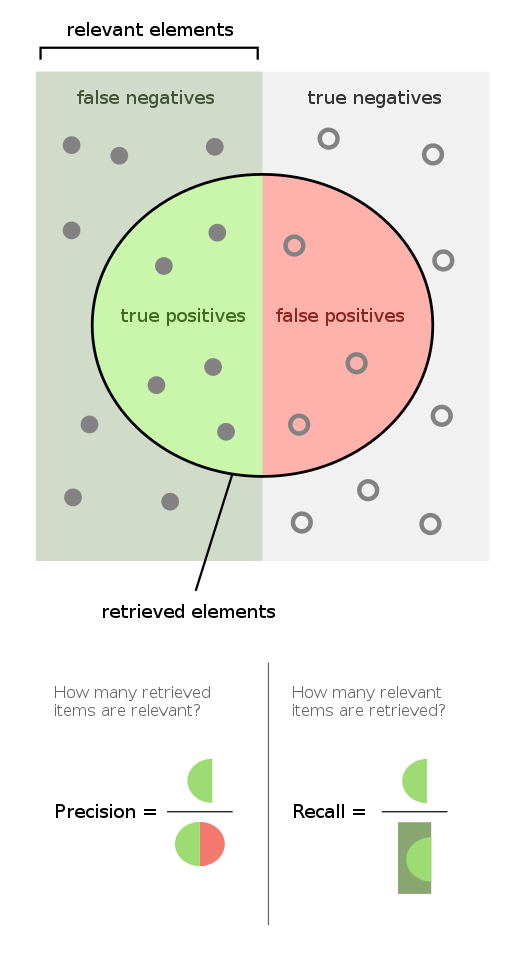
\includegraphics[width=0.5\linewidth]{graphics//chapter3/Precisionrecall.svg.png}
        \caption{Precision and Recall}
        \label{fig:precision-recall}
    \end{figure}
    From the above definitions of Precision and Recall, we can say that recall determines the performance of a classifier with respect to a false negative, whereas precision gives information about the performance of a classifier with respect to a false positive.\par\vspace{1em}
    So, if we want to minimize the false negative, then, Recall should be as near to 100\%, and if we want to minimize the false positive, then precision should be close to 100\% as possible.In simple words, if we maximize precision, it will minimize the FP errors, and if we maximize recall, it will minimize the FN error.
    
    \subsection{F1 Score}
    F-score or F1 Score is a metric to evaluate a binary classification model on the basis of predictions that are made for the positive class. It is calculated with the help of Precision and Recall. It is a type of single score that represents both Precision and Recall. So, the F1 Score can be calculated as the harmonic mean of both precision and Recall, assigning equal weight to each of them.\par \vspace{1em}

    The formula for calculating the f1 score is given below\cite{c-eval}: 
    \begin{center}
        \(\displaystyle{\text{F1 Score} = 2 * \frac{\text{precision} * \text{recall}}{\text{precision} + \text{recall}}}\) 
    \end{center}

    \subsection{When to use F-Score}
    As F-score make use of both precision and recall, so it should be used if both of them are important for evaluation, but one (precision or recall) is slightly more important to consider than the other. For example, when False negatives are comparatively more important than false positives, or vice versa.\\par \vspace{1em}
    
    % \subsection{Importance Precision vs Recall Trade-off }
    % Both precision and recall may be useful in cases where there is imbalanced data. However, it may be valuable to prioritize one over the other in cases where the outcome of a false positive or false negative is costly. For example, in medical diagnosis, a false positive test can lead to unnecessary treatment and expenses. In this situation, it is useful to value precision over recall. In other cases, the cost of a false negative is high. For instance, the cost of a false negative in fraud detection is high, as failing to detect a fraudulent transaction can result in significant financial loss.\par\vspace{1em}
    
    % \textbf{Trade-off Scenarios}
    % \begin{enumerate}
    %     \item \textbf{High Precision, Low Recall:} This scenario is favorable in situations where false positives are costly. For instance, in spam detection, high precision ensures that non-spam emails are rarely misclassified as spam.
    %     \item \textbf{High Recall, Low Precision:} This scenario is preferable when missing a positive case is more detrimental. In medical diagnosis, high recall ensures that most patients with the disease are correctly identified, even if some healthy individuals are incorrectly flagged.
    % \end{enumerate}
    % Balancing precision and recall is crucial for applications requiring a compromise between the two, such as fraud detection or information retrieval systems.


    % \subsection{F1-Score as a Balanced Metric}
    % The F1-Score provides a single metric that balances precision and recall, particularly useful when the class distribution is imbalanced.\par\vspace{1em}
    % The F1-Score is the harmonic mean of precision and recall, emphasizing that both metrics are equally important. Unlike the arithmetic mean, the harmonic mean penalizes extreme values more, ensuring that both precision and recall need to be sufficiently high to achieve a high F1-Score.\par\vspace{1em}

    % \textbf{Benefits of F1-Score}
    % \begin{itemize}
    %     \item Balanced Evaluation: It balances the importance of both false positives and false negatives.
    %     \item Imbalanced Datasets: It is particularly useful for imbalanced datasets where accuracy might be misleading.
    %     \item Unified Metric: It provides a single, interpretable metric to evaluate the model's performance.
    % \end{itemize}




 
\chapter{Dataset}

This chapter describe the \textbf{Plant Village datasets} that we used in our work.\par\vspace{1em}


\section{PlantVillage Dataset}

    \subsection{Overview}
    PlantVillage is a dataset consisting of 54303 healthy and unhealthy leaf images divided into 38 classes by species and disease.
    \begin{figure}
        \centering
        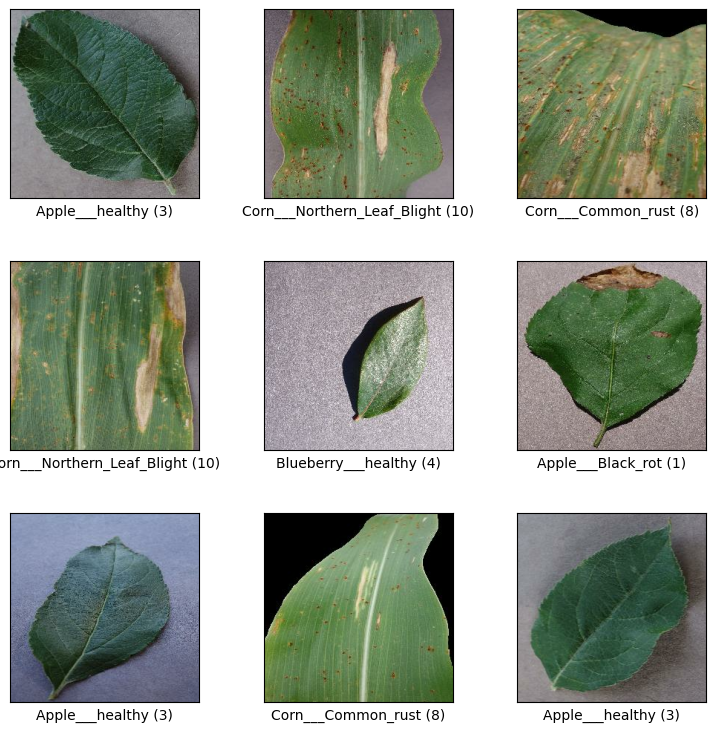
\includegraphics[width=\linewidth]{graphics//chapter 4/plant village dataset viz.png}
        \caption{Plant Village Datasets}
        \label{fig:plant village vizl}
    \end{figure}
    
    \subsection{Original classes and labels}
        It consists of the following 38 classes and has a total of 54303 items.

    \begin{figure}
        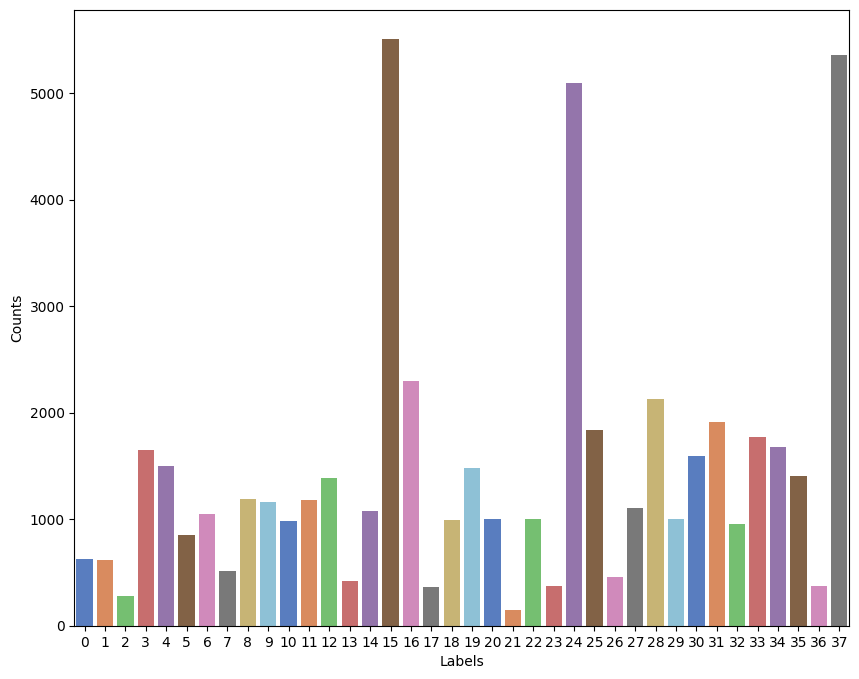
\includegraphics[width=1\linewidth]{graphics//chapter 4/38 class distribution.png}
        \caption{Class Distribution Before Class Reduction}
        \label{Class Distribution Before Class Reduction}
    \end{figure}

    
    \begin{multicols}{2}
    \begin{enumerate}
    \item Apple\_scab
    \item Apple\_black\_rot
    \item Apple\_cedar\_apple\_rust
    \item Apple\_healthy
    \item Background\_without\_leaves
    \item Blueberry\_healthy
    \item Cherry\_powdery\_mildew
    \item Cherry\_healthy
    \item Corn\_gray\_leaf\_spot
    \item Corn\_common\_rust
    \item Corn\_northern\_leaf\_blight
    \item Corn\_healthy
    \item Grape\_black\_rot
    \item Grape\_black\_measles
    \item Grape\_leaf\_blight
    \item Grape\_healthy
    \item Orange\_haunglongbing
    \item Peach\_bacterial\_spot
    \item Peach\_healthy
    \item Pepper\_bacterial\_spot
    \item Pepper\_healthy
    \item Potato\_early\_blight
    \item Potato\_healthy
    \item Potato\_late\_blight
    \item Raspberry\_healthy
    \item Soybean\_healthy
    \item Squash\_powdery\_mildew
    \item Strawberry\_healthy
    \item Strawberry\_leaf\_scorch
    \item Tomato\_bacterial\_spot
    \item Tomato\_early\_blight
    \item Tomato\_healthy
    \item Tomato\_late\_blight
    \item Tomato\_leaf\_mold
    \item Tomato\_septoria\_leaf\_spot
    \item Tomato\_spider\_mites\_two-spotted\_spider\_mite
    \item Tomato\_target\_spot
    \item Tomato\_mosaic\_virus
    \item Tomato\_yellow\_leaf\_curl\_virus
    \end{enumerate}
    \end{multicols}

    \vspace{1em}

    \subsection{Classes used}
    We have narrowed down these 38 classes to 11 classes, because of hardware constraints.\par \vspace{1em}

    
    
    The narrowed-down classes, totaling 10431 items are:

    \begin{multicols}{2}
    \begin{enumerate}
    \item Apple\_Apple\_scab
    \item Apple\_Black\_rot
    \item Apple\_Cedar\_apple\_rust
    \item Apple\_healthy
    \item Blueberry\_healthy
    \item Cherry\_healthy
    \item Cherry\_Powdery\_mildew
    \item Corn\_Cercospora\_leaf\_spot\_Gray\_leaf\_spot
    \item Corn\_Common\_rust
    \item Corn\_healthy
    \item Corn\_Northern\_Leaf\_Blight
    \end{enumerate}
    \end{multicols}

    \subsection{Item Data Composition}
    The original PlantVillage data was mildly imbalanced as such, our dataset also suffers from mild data imbalance.

    \begin{figure}
        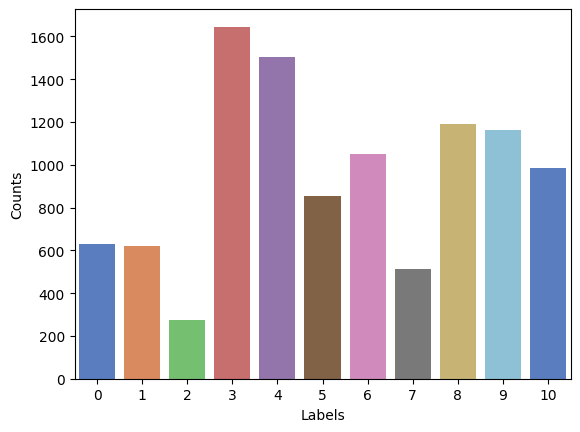
\includegraphics[width=0.8\textwidth, center]{graphics/chapter 4/Image_Classifications.png}
        \caption{Class distribution after class reduction}
    \end{figure}
     \par \vspace{1em}
     
    Key:
    \begin{multicols}{2}
    \begin{enumerate}
        \setcounter{enumi}{-1}
        \item Apple\_Apple\_scab
        \item Apple\_Black\_rot
        \item Apple\_Cedar\_apple\_rust
        \item Apple\_healthy
        \item Blueberry\_healthy
        \item Cherry\_healthy
        \item Cherry\_Powdery\_mildew
        \item Corn\_Cercospora\_leaf\_spot\_Gray\_leaf\_spot
        \item Corn\_Common\_rust
        \item Corn\_healthy
        \item Corn\_Northern\_Leaf\_Blight
    \end{enumerate}
    \end{multicols}

    \vspace{2em}

    A potential solution to imbalanced classes is to use either:
    \begin{enumerate}
        \item Downsampling (in this context) means training on a disproportionately low subset of the majority class examples.
        \item Upweighting means adding an example weight to the downsampled class equal to the factor by which you downsampled
    \end{enumerate}

    

    

    
    % \item Classes and labels - List of Plant Species and Associated Diseases, 36 11
    
    % \item Number of Classes (11 in total)
    
    % \item Data Composition - Number of Images per Class, Image Resolutions and Formats, Distribution of Images across Classes
    % \item Example Images - Visual Examples of Images from Different Classes,
    %% \item Variability in Image Quality and Conditions


\par

\newpage
\section{Data Processing Techniques}

\begin{enumerate}
    \item Image Augmentation - Importance of Augmentation in Preventing Over fitting
    \item Techniques Used (e.g., Rotation, Flipping, Zooming, Cropping)
    \item Data Preprocessing for each model VGG16, Xception, MobilenetV2
    \item Data Splitting - Training, Validation, and Test Split Ratios, Stratified Splitting to Maintain Class Distribution, Rationale for Chosen Split Ratios
    \item Handling Class Imbalance - Techniques for Managing Imbalanced Data - (e.g., Oversampling, Undersampling) Impact on Model Training and Evaluation
\end{enumerate}
\par

\subsection{Image Augmentation}
A technique used to artificially increase the training set by creating modified copies of a dataset using existing data. This technique is very useful when an image dataset is small. This also helps expose our model to different aspects of the training data and reduce overfitting. \par \vspace{1em}
We implement this process by adding an Augmentation Layer to our classifier models.
Augmentation Layer are only active during training and not during model’s inference or evaluation.\par \vspace{1em}
Our Augmentation Layer includes: RandomFlip, RandomRotation, Saturation, Brightness

\begin{figure}
    \centering
    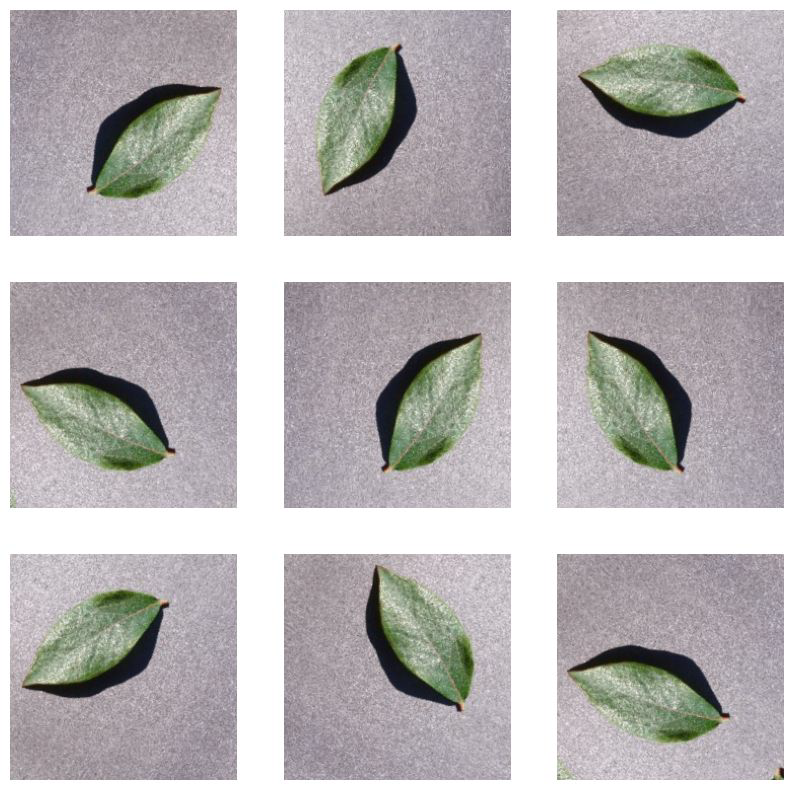
\includegraphics[width=1\linewidth]{graphics//chapter 4/image aug.png}
    \caption{Image Augmentation}
    \label{fig:img-augmentation}
\end{figure}


\subsection{Data Splitting}
The total of 10431 images are split 80:10:10, which is:\par
80\% in training, i.e. 8344 images for actual training.\par
10\% for testing, i.e. 1044 images for testing.\par
10\% for validation, i.e. 1044 images for validating the result.\par \vspace{1em}

Data Splitting is important as it helps prevent overfitting, ensure robustness and generalization.

\begin{figure}
    \centering
    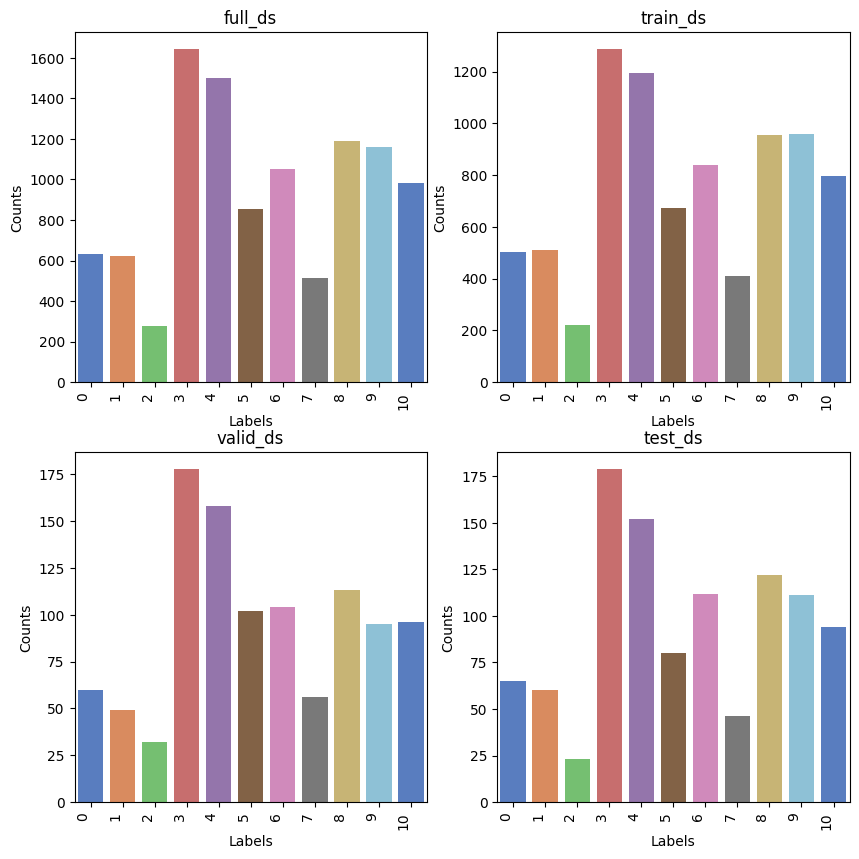
\includegraphics[width=1\linewidth]{graphics//chapter 4/train test split.png}
    \caption{Train, Test, Validation Split}
    \label{fig:train-test-split}
\end{figure}

\newpage





\chapter{Methodology}

In this chapter, we provide the detail procedures, steps that we have done in our research and how our results are obtained.\par\vspace{1em}


\section{Building pre-trained classifier model}
\begin{figure}
    \centering
    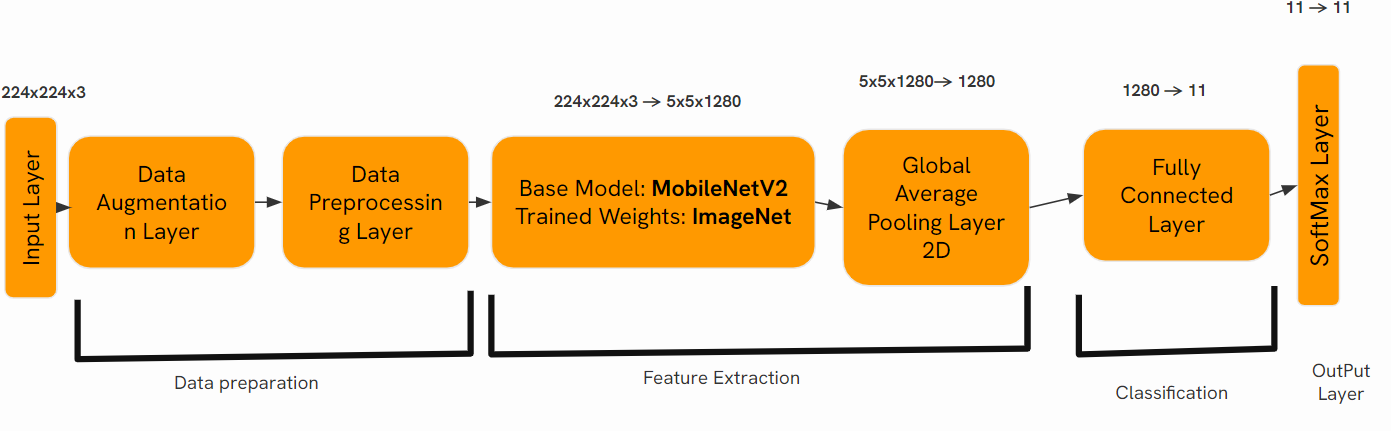
\includegraphics[width=1\linewidth]{graphics/chapter5/mobileNetV2 base model.png}
    \caption{MobileNetV2 Based Model}
    \label{fig:mobilenetv2-based-model}
\end{figure}

For building our model for performing transfer learning, we take the following steps.\\
We first build our data preprocessing pipeline which involves batching our images inorder to perform prediction, inference, prediction faster, resizing our image datasets to a desired shape that can be accepted by our model. After that, we load our pre-trained model by removing their top layers and added a single Fully Connected Layers (FCN) layer which have which have size equal to the number of classes that we want to perform classifications on.\par\vspace{1em}

For building our pre-trained classifier model, with MobileNetV2, refer fig\ref{fig:mobilenetv2-based-model} as base model, we first download the pretrained MobileNetV2 model with weights trained on \textbf{ImageNet datasets} and remove their top layers. Then, we add a \textbf{Global Average Pooling 2D Layer} on the top of the downloaded pretrained model to flatten the  7x7x1280 features map extracted by the base model, by taking the average of each 7 x 7 features map. Now, we add a single \textbf{FCN Layer} on top of Global Avg Pool 2D layer as the last layer. The number of neuron units in this FCN Layer is equal to 11 units as we are planning to classify 11 classes,\par\vspace{1em}

Similarly, we build other pretrained model using VGG-16 and Xception as base model, using the same procedures as above. The detailed description of each model layer is shown in fig \ref{fig:mob-vgg16-base-model} and \ref{fig:xception-base-model}.

\begin{figure}
     \begin{subfigure}{\linewidth}
        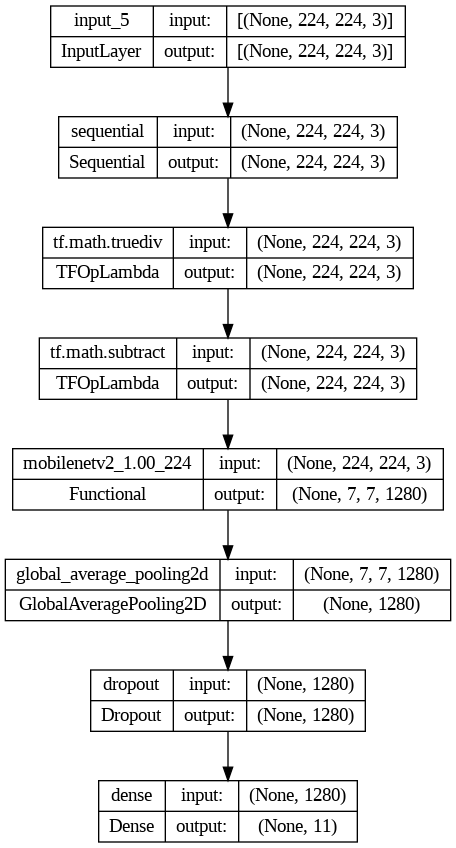
\includegraphics[width=.5\linewidth]{graphics/chapter5/mobilnetV2 based model graph.png}\hfill
        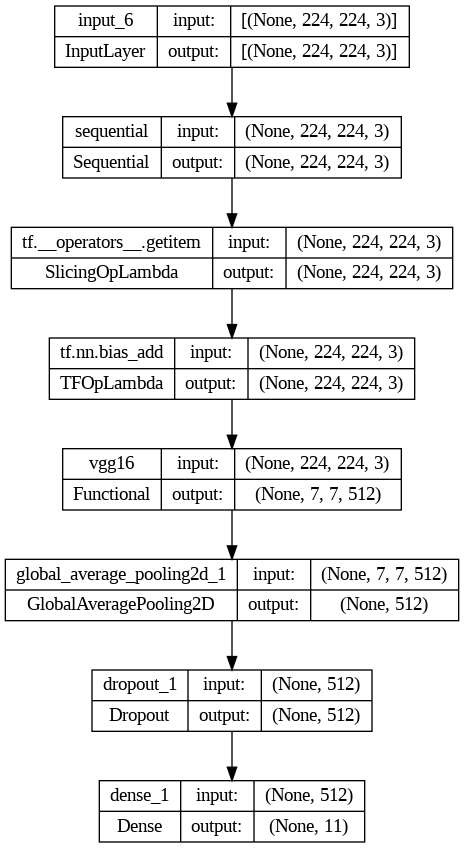
\includegraphics[width=.5\linewidth]{graphics//chapter5/vgg16 base model graph.png}\hfill
    \end{subfigure}    
    \caption{From left to right: MobilNetV2 Base Model, VGG-16 Base Model}
        \label{fig:mob-vgg16-base-model}    
\end{figure}

\begin{figure}
    \centering
    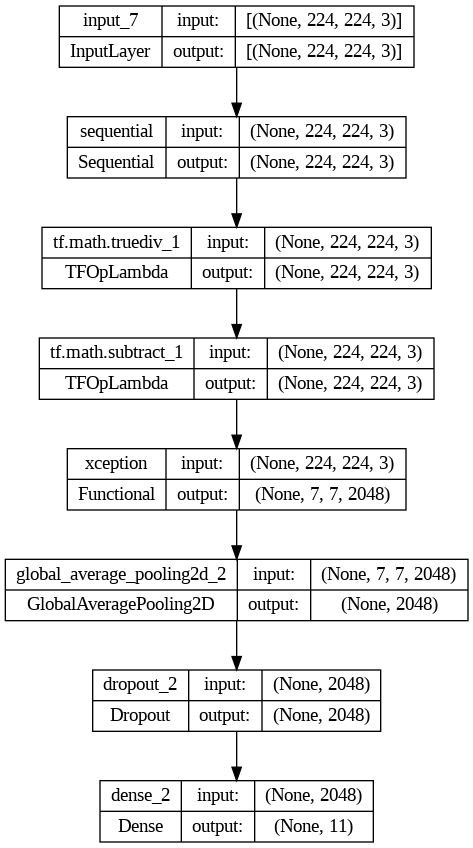
\includegraphics[height=\textheight]{graphics//chapter5/xception base model graph.png}
    \caption{Xception Base Model}
    \label{fig:xception-base-model}
\end{figure}


\section{Transfer Learning}\label{Transfer-learning-section}

\begin{figure}
    \centering
    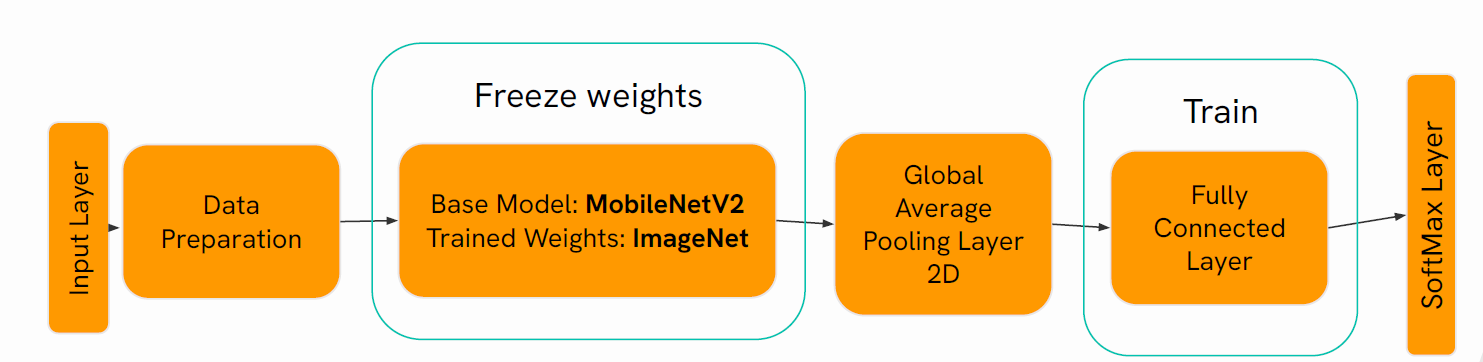
\includegraphics[width=\linewidth]{graphics//chapter5/transfer learning.png}
    \caption{Transfer Learning}
    \label{fig:transfer-learning}
\end{figure}

After building our MobileNetV2, VGG16, Xception base model, we start performing transfer learning and fine-tuning our models using our datasets. So, we first split our datasets on \textbf{80:10:10} ratios corresponding to training, testing and validation datasets size.\par\vspace{1em}

Then, we perform transfer learning by using the following approach, we freeze the weights of the entire base model, (i.e VGG16. Xception, MobileNetV2 part of our model), then we start training only the FCN layer of our models. Here, Freezing is a technique to prevents the weights in a given layer from being updated during training In this way, we trained our model without destroying the weights (knowledge) that it has learned previously (learned from \textbf{ImageNet datasets})\\
So, in transfer learning phase of the training, we just used our base model as a feature extractor and trained only the last top layer (FCN layer) that we added, to perform the classification task using the features extracted by the base model. 


\subsection{Model Training}

\begin{figure}
    \centering
    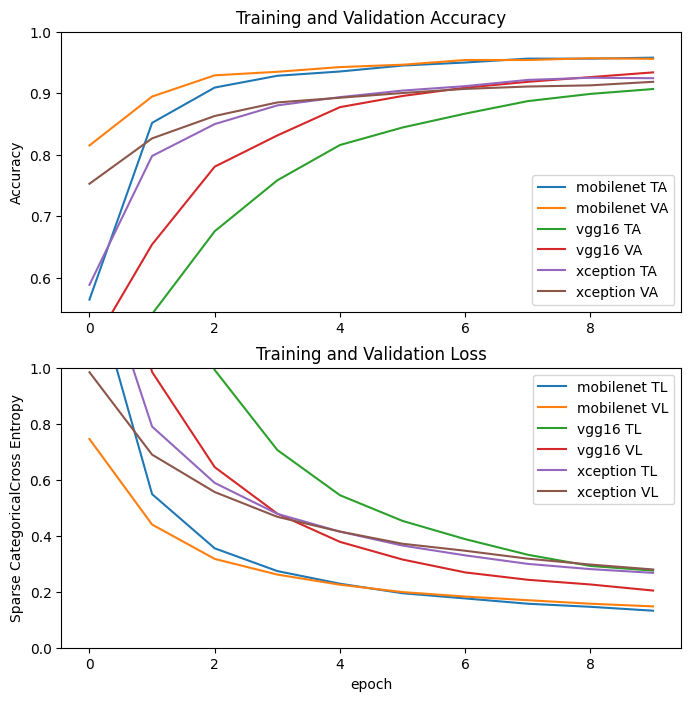
\includegraphics[width=1\linewidth]{graphics//chapter5/transfer learning training.png}
    \caption{Transfer Learning Training Graph}
    \label{fig:transfer-learning-training}
\end{figure}

\textbf{Parameters}:\par
\begin{itemize}
    \item \textbf{Epochs}: 10\par
    \item \textbf{Learning Rate}: $10^{-4}$\par
    \item \textbf{Loss Function}: Sparse Categorical Cross Entropy\par
    \item \textbf{Optimizer}: Adam\par
    \item \textbf{Metrics}: Accuracy
\end{itemize}


In the transfer learning phase, we observe that while training our model, MobileNetV2 base model converse fastest as compared to other models. So, we can say that MobileNetV2 is an excellent feature extractor as compared to the other 2 models that we used.


\section{Fine Tuning}
\textbf{Parameters}
\begin{itemize}
    \item \textbf{Epochs}: 10
    \item \textbf{Learning Rate}: $10^{-5}$
    \item \textbf{Loss Function}: Sparse Categorical Cross Entropy
    \item \textbf{Optimizer}: RMSProp
    \item \textbf{Metrics}: Accuracy
\end{itemize}


\begin{figure}
    \centering
    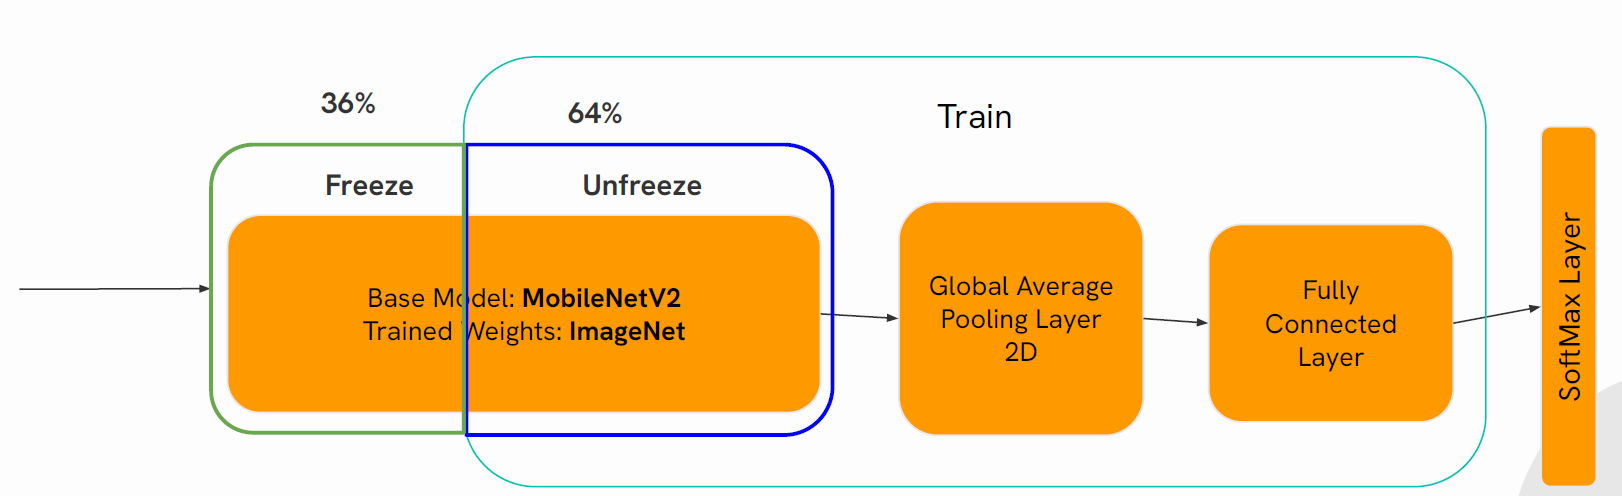
\includegraphics[width=1\linewidth]{graphics//chapter5/fine tuning.png}
    \caption{Fine Tuning}
    \label{fig:fine-tuning}
\end{figure}

We perform the fine-tuning phase of our model just after transfer learning phase, this phase of training is performed mainly to further increase the performance of our model on our particular training datasets.\\

In transfer learning, we were only training the top layers of our base model. The weights of the pre-trained network were not updated during training. One way to increase performance even further is to train (or "fine-tune") the weights of the top layers of the pre-trained model alongside the training of the classifier we added. The training process will force the weights to be tuned from generic feature maps to features associated specifically with the dataset.\par\vspace{1em}

Fine tuning of our model on Plant Village Datasets is perform in the following ways, we first unfreeze 64\% of the top layers of our base models and freeze the remaining 36\% of our model weights. Then, we again trained our model with our datasets with the unfreeze weights and the last FCN layer. \par\vspace{1em}

While fine tuning, we should try to fine-tune a small number of top layers rather than the whole base model layers. 
The reason why we unfreeze 64\% top layer of our base model and not unfreeze the entire base model weights is because in most convolutional networks, the higher up a layer is, the more specialized it is. The first few layers learn very simple and generic features that generalize to almost all types of images. As you go higher up, the features are increasingly more specific to the dataset on which the model was trained. The goal of fine-tuning is to adapt these specialized features to work with the new dataset, rather than overwrite the generic learning.\par\vspace{1em}

\subsection{Model Training}

\begin{figure}
    \centering
    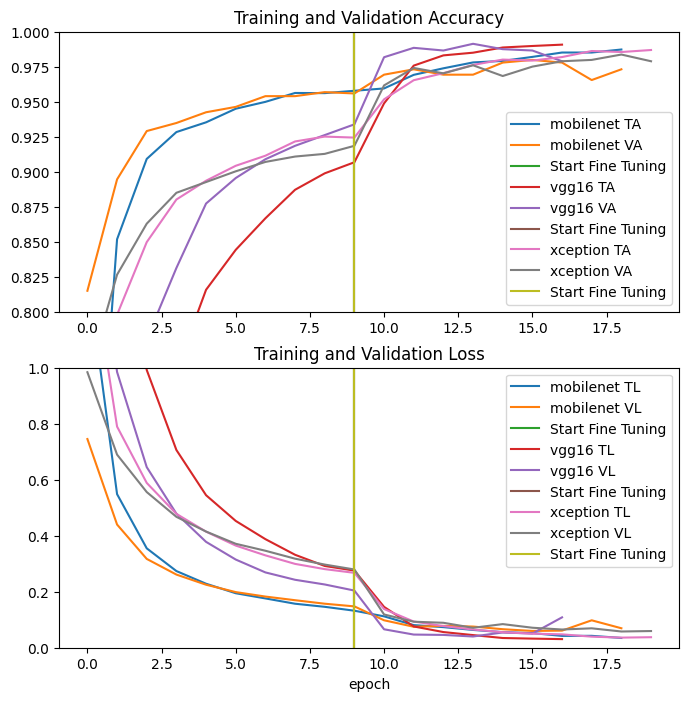
\includegraphics[width=1\linewidth]{graphics//chapter5/fine tuning training graph.png}
    \caption{Fine Tuning Training Graph}
    \label{fig:fine-tuning-training}
\end{figure}


During the fine-tuning phase of our model, we observe from the training curve graph, that the VGG-16 base model converges faster and outperforms other other models. So we can inferred that VGG-16 model can generalized well on specific datasets using its learned knowledge. \par\vspace{1em}

The success of VGG16 indicates that the pre-trained weights on ImageNet were highly beneficial and effectively transferable to the Plant Village dataset. VGG16’s architecture, with its deep layers, is adept at extracting intricate and hierarchical features, which are crucial for distinguishing between different plant diseases.\par\vspace{1em}

 The ability of VGG16 to effectively adapt pre-trained features to new data highlights the power of transfer learning and fine-tuning in achieving high accuracy and robust model performance. \par\vspace{1em}
 

\section{CNN10L ConvNet Model}
 We build our CNN10L Model using the specifications define in \ref{fig:CNN10L} and \ref{fig:cnn10l-detail-arch} 
 
\subsection{Model Training}
We trained our CNN10L model using \textbf{K Fold Cross Validation Method}. \\

So, in this technique, we first divide our dataset into train and test split in ratio of 90:10. Then, further divide our training set into K folds. After that, we perform K fold Cv Training of our model.
In the first phase (i.e. K = 1), we take the last fold as validation set and remaining as training set and perform training. Then in second K fold training phase (i.e. K = 2), we take the last second fold as validation set and remaining folds as training sets and again train our models. Similarly , we continue this process for K times taking $K^{th}$ fold as validation step. The steps for this training is shown clearly in the figure \ref{fig:k-fold}\par\vspace{1em}

\textbf{Parameters}:
\begin{itemize}
    \item \textbf{K }= 5 folds
    \item \textbf{Epochs:} 30 (with Early Stopping Condition)
    \item \textbf{Learning Rate:} $10^{-3}$
    \item \textbf{Loss Function:} Sparse Categorical Cross Entropy
    \item \textbf{Optimizer:} Adam
    \item \textbf{Metrics:} Accuracy
\end{itemize}

The training curve for our CNN10LL model for 5 K folds is shown in fig\ref{fig:cnn10l-fold1-3} and \ref{fig:cnn10l-fold4-5}\par\vspace{1em}

\begin{figure}
    \centering
    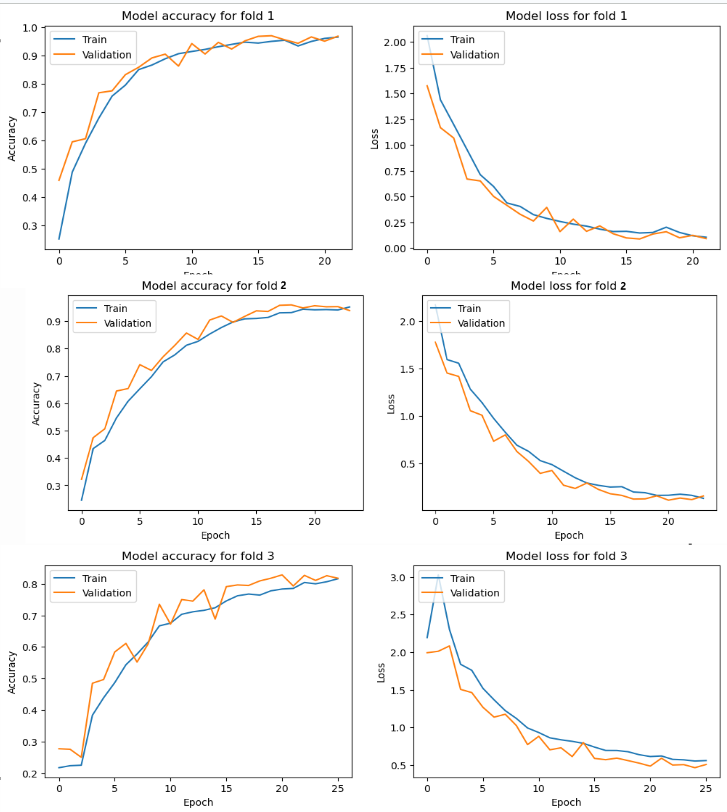
\includegraphics[width=1\linewidth]{graphics//chapter5/cnn10L training fold1-3.png}
    \caption{CNN10L Training for fold 1 to fold 3}
    \label{fig:cnn10l-fold1-3}
\end{figure}

\begin{figure}
    \centering
    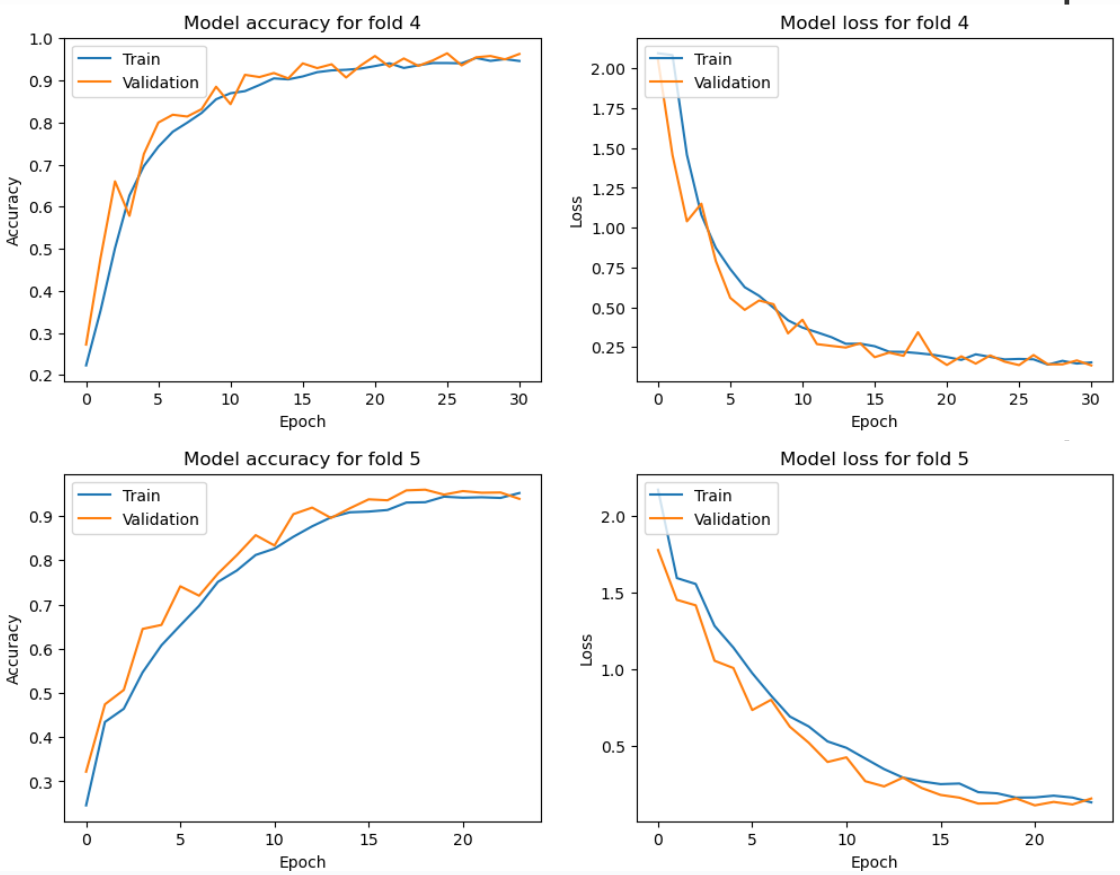
\includegraphics[width=1\linewidth]{graphics//chapter5/cnn10L training fold4-5.png}
    \caption{CNN10L Training for fold 4 to fold 5}
    \label{fig:cnn10l-fold4-5}
\end{figure}

\FloatBarrier


\section{Classical ML model as Classifier}

    \begin{figure}
        \centering
        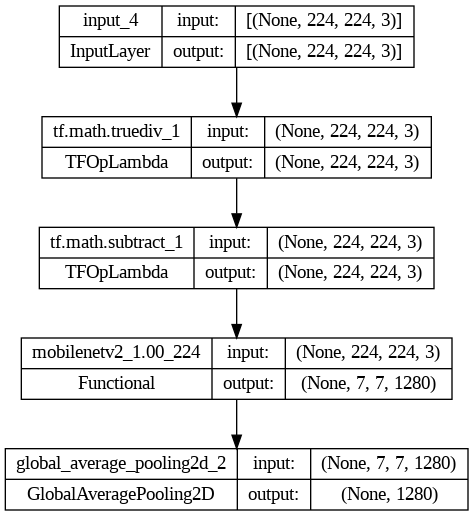
\includegraphics[width=0.75\linewidth]{graphics//chapter5/moboilenetv2 feature extractor.png}
        \caption{MobileNetV2 Feature Extractor used for training Classic ML Model}
        \label{fig:mobnetv2-feature-extractor}
    \end{figure}

\begin{figure}
    \centering
    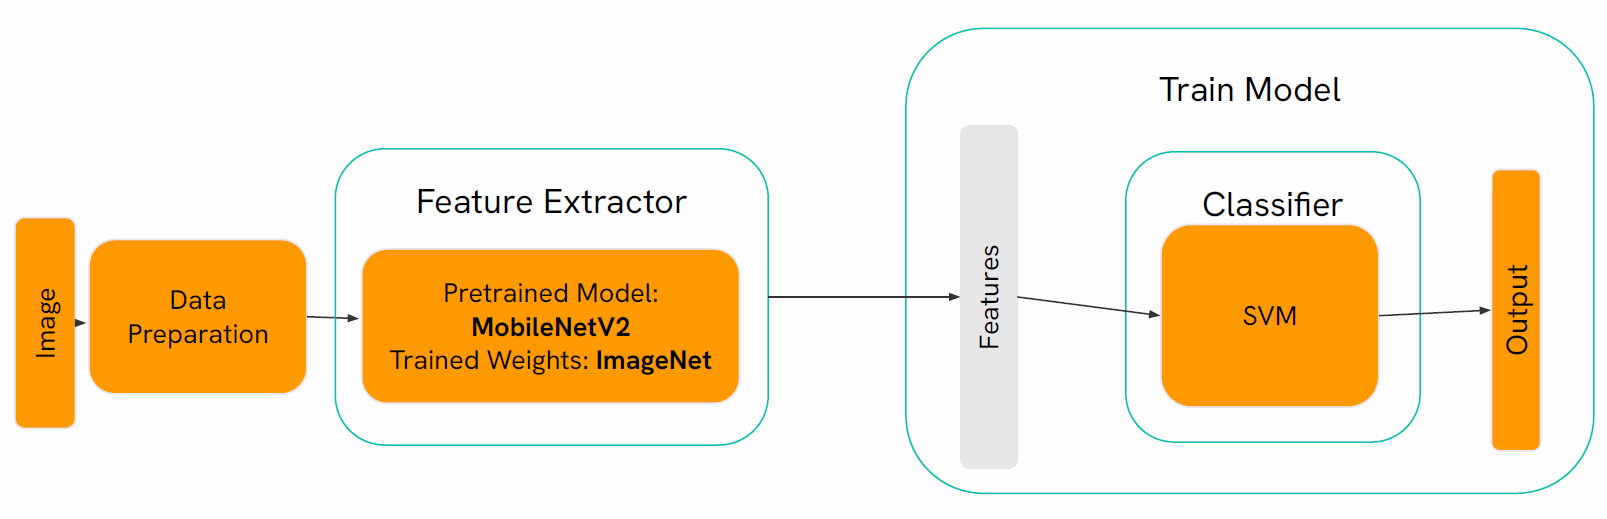
\includegraphics[width=1\linewidth]{graphics//chapter5/mobilenetV2 + SVM.png}
    \caption{MobilenetV2 + SVM}
    \label{fig:mobilenetv2-svm}
\end{figure}

\begin{figure}
    \centering
    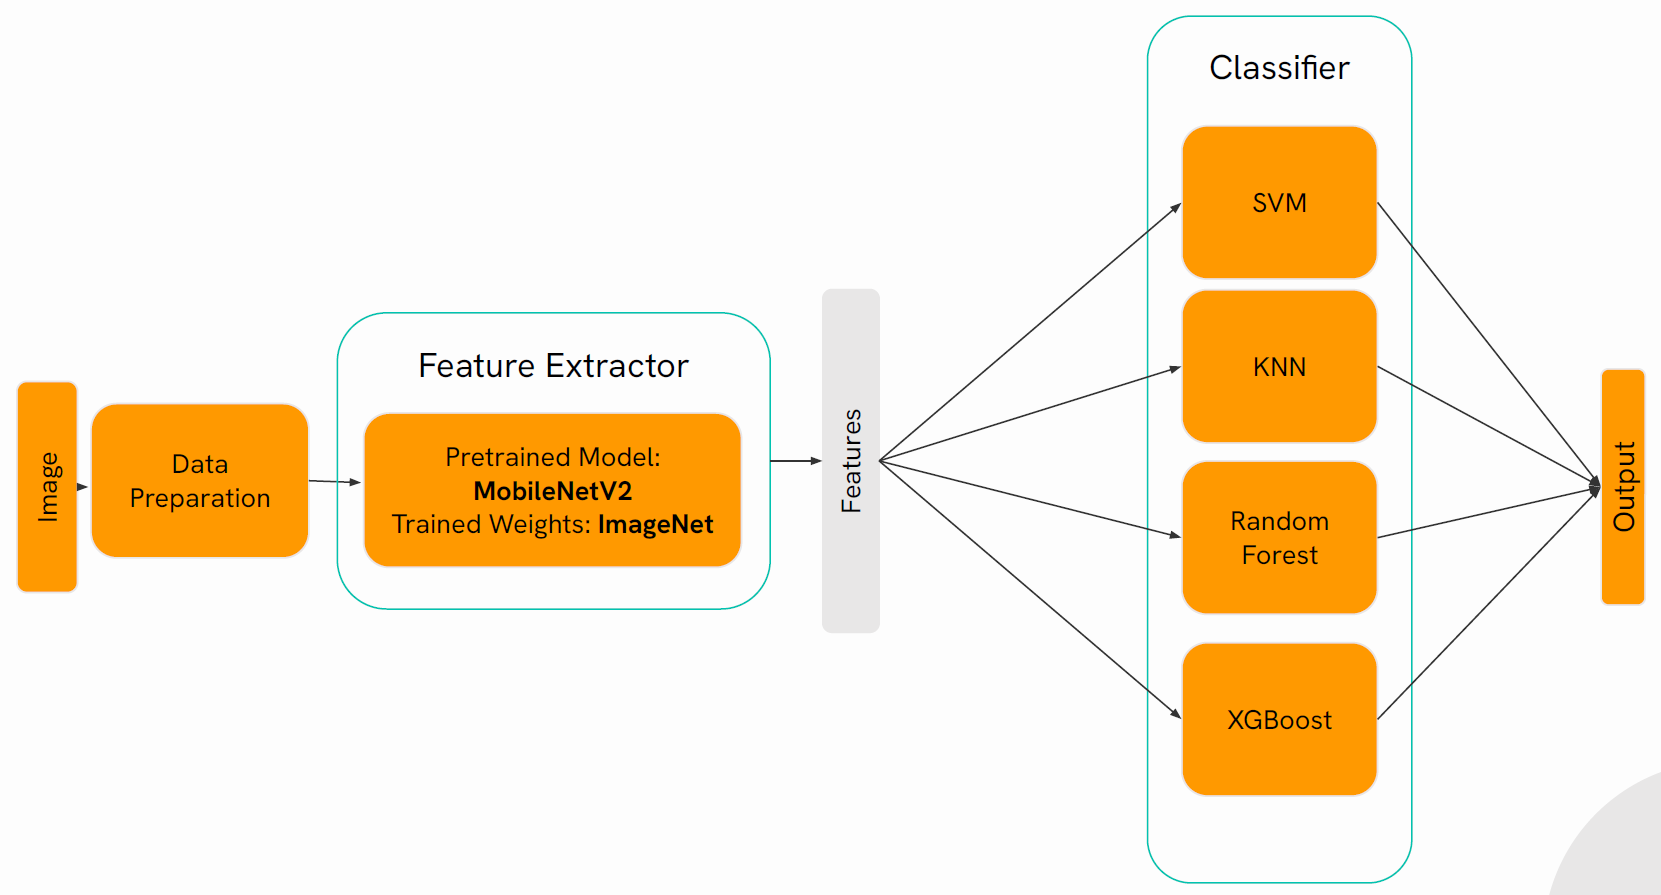
\includegraphics[width=1\linewidth]{graphics//chapter5/mobilentV2 + ML.png}
    \caption{MobileNetV2 + Traditional Classifier Models}
    \label{fig:mobilenetv2-all}
\end{figure}

    Since, classical ML classifier models such as SVM, KNN, Random forest, XBoost, etc cannot extract features directly from an image, we used a pretrained MobileNetV2 as a feature extractor for training these models.\par\vspace{1em}

    So, we first download a pretrained MobileNetV2 model (trained on \textbf{ImageNet}) and remove its top layer so that it gives the last feature maps as an output instead of the 1000 classes outputs. 
    Then, we input an image to this MobileNetV2, which give out a 7 x 7 x 1280 features map. we perform a global average pooling 2d on this output feature map to produce a 1280 features vector (7 x 7 x 1280 to 1 x 1 x 1280). \par\vspace{1em}
    In this way, we perform feature extraction for all the images in our dataset to convert it into 1280 feature vectors from an image of shape 256 x 256 x 3, then train our traditional classifier model on this extracted features
\FloatBarrier




\chapter{Result}

This chapter presents the results of our comparative study on various image classification models using the Plant Village dataset. We detail the performance metrics of each model, highlighting the strengths and weaknesses observed through their evaluation. \par\vspace{1em}
\par\vspace{1em}


\section{Comparative Analysis of Models}

In this chapter, we explain the performance of different models that we used in our research with the help of graphs, tables, etc

\subsection{Pretrained Model Accuracy and Loss Comparison After Transfer Learning}
\begin{figure}
    \centering
    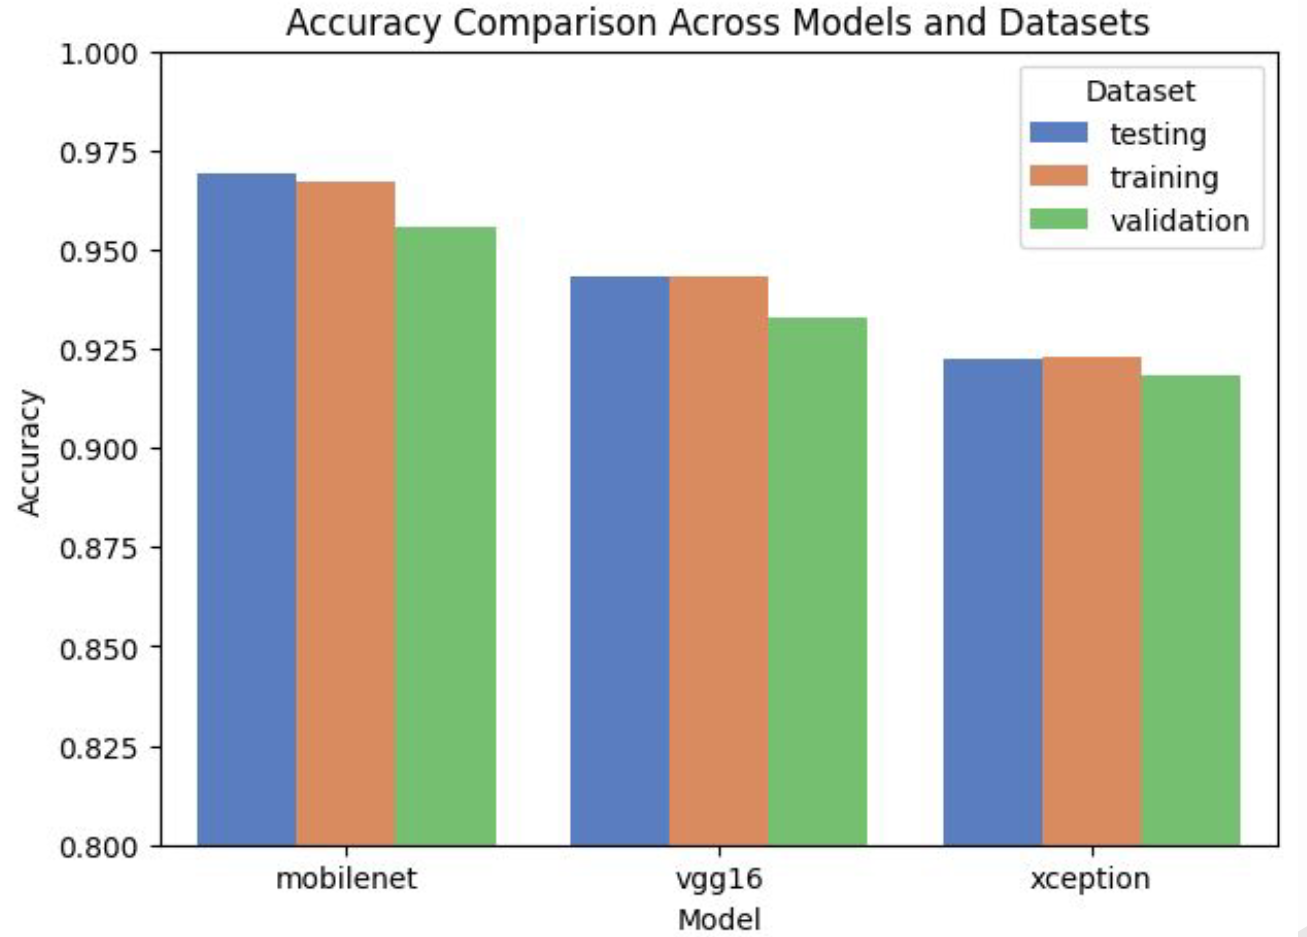
\includegraphics[width=0.75\linewidth]{graphics//chapter6/transfer learning acc.png}
    \caption{Pretrained Model Accuracy After Transfer Learning}
    \label{fig:acc-tf}
\end{figure}

\begin{figure}
    \centering
    \includegraphics[width=0.75\linewidth]{graphics//chapter6/model loss transfer learning.png}
    \caption{Pretrained Model Loss After Transfer Learning}
    \label{fig:loss-tf}
\end{figure}

After performing transfer learning of our pretrained Convnet models, we observe that MobileNetV2 outperforms all other models with an accuracy of\textbf{\textit{ (0.9670, 0.95589, 0.9693)}} on training, validation and testing datasets, respectively. But, the performance difference between the models is very low, they all perform very well with very little difference. \par\vspace{1em}
As we have already mentioned in methodology section \ref{Transfer-learning-section}, that in transfer learning we are not touching any weights of the base model only the last FCN layer is trained, So, we can inferred from this observation that MobileNetV2 is an excellent feature extractor for generally all classes, even for narrow domain. This is the reason, why we used MobileNetV2 as an feature extractor in combination with other traditional classifeir instead of other convnet model (eg: VGG16, Xception) 
\par\vspace{1em}

% \FloatBarrier


\subsection{Pretrained Model Accuracy and Loss Comparison After Fine Tuning}
\begin{figure}
    \centering
    \includegraphics[width=0.75\linewidth]{graphics//chapter6/pretrained acc after fine tuning.png}
    \caption{Pretrained Model Accuracy After Fine Tuning}
    \label{fig:acc-ft}
\end{figure}

\begin{figure}
    \centering
    \includegraphics[width=0.75\linewidth]{graphics//chapter6/model loss after fine tuning.png}
    \caption{Pretrained Model Loss after Fine Tuning}
    \label{fig:loss-ft}
\end{figure}

When performing fine tuning the models, we observe that  VGG16 base model, outperform  other models even MobileNet. However, the difference in model accuracy with these 3 models, is very low, they only differ by about 1\% in their accuracy. So, we can say they perform in par with each other.\par\vspace{1em}

% \FloatBarrier

\subsection{Model Comparison with our CNN10L Model}
When comparing our CNN10L model (model that we trained from scratch), against the three pre-trained deep learning models: MobileNetV2, VGG16, and Xception, we observed that the CNN10L model perform badly in all classification evaluation metrics but not by much. In term of accuracy metric, CNN10L get (0.9648, 0.9681, 0.952107) in comparison to the best performing model  (0.9917, 0.9913, 0.9913) in training, validation and testing datasets, respectively.
\par\vspace{1em}
\begin{figure}
    \centering
    \includegraphics[width=1\linewidth]{graphics//chapter6/nn model acc.png}
    \caption{Neural Network Model Accuracy Comparisons}
    \label{fig:nn-acc}
\end{figure}

\begin{figure}
    \centering
    \includegraphics[width=1\linewidth]{graphics//chapter6/nn loss comparison.png}
    \caption{Neural Network Model Loss Comparisons}
    \label{fig:nn-loss}
\end{figure}

% \FloatBarrier

\subsection{Comparison of all model using different evaluation metrics}
 In this section, we perform comparison of all the models that we used.
 \par\vspace{1em}
 The highest accuracy model from our comparison was VGG16, which is a pretrained model, with 0.99 accuracy. Our custom model got an accuracy rating of 0.95. The least accurate model was a traditional model utilizing RandomForest yielding an accuracy rating of 0.84 in accuracy of testing dataset.
 \par\vspace{1em}
 
After these rigorous comparisons between the various models using different evaluation matrices, the consensus is that pre-trained deep learning models have a noticeable increase in performance and accuracy, over model trained from scratch and  traditional models. Pre-trained models also have some increase in performance and accuracy over our custom trained model, CNN10L.\par \vspace{1em}

From this observation, we inferred that, the knowledge that is learned by pretrained model from large datasets like ImageNet is actually helpful in performing classification in narrow domain tasks as our scratch model, CNN10L is easily outperform by the 3 pretrained base model in term of accuracy, precision, recall and F1-score.
\par\vspace{1em}
Among traditional classifier models, we observe that SVM and XGBoost perform the best and Random Forest is the worst-performing one. Even though CNN10L outperform  traditional classifier, the difference in metrics score is very small (3\% difference in accuracy metric) with the best performing traditional classifier model (SVM and XGBoost). So, we can say that these classical models are in par with neural network models and we should not completely ignore them. 
\par\vspace{1em}



\newgeometry{left=1cm,right=1cm}
\begin{table}[h]
    \centering
    \resizebox{\textwidth}{!}{%
    \begin{tabular}{lccccccccccccc}
        \toprule
        \textbf{Model} & \textbf{Measure} & \multicolumn{11}{c}{Classes} & \textbf{Accuracy}\\
         &  & \textbf{0} & \textbf{1} & \textbf{2} & \textbf{3} & \textbf{4} & \textbf{5} & \textbf{6} & \textbf{7} & \textbf{8} & \textbf{9} & \textbf{10}\\
         
        \midrule
        
        \textbf{MobileNetV2} & \textbf{Precision} & \textbf{1.00} & \textbf{1.00} & \textbf{0.96} & \textbf{1.00} & \textbf{1.00} & \textbf{1.00} & \textbf{1.00} & \textbf{1.00} & \textbf{1.00} & \textbf{1.00} & \textbf{0.86} & \textbf{}\\
        \textbf{} & \textbf{Recall} & \textbf{1.00} & \textbf{1.00} & \textbf{0.96} & \textbf{1.00} & \textbf{1.00} & \textbf{1.00} & \textbf{1.00} & \textbf{0.88} & \textbf{1.00} & \textbf{1.00} & \textbf{0.99} & \textbf{}\\
        \textbf{} & \textbf{F1-Score} & \textbf{1.00} & \textbf{1.00} & \textbf{0.98} & \textbf{1.00} & \textbf{1.00} & \textbf{1.00} & \textbf{1.00} & \textbf{0.88} & \textbf{1.00} & \textbf{1.00} & \textbf{0.92} & \textbf{0.99}\\
        \textbf{} & \textbf{Support} & \textbf{63} & \textbf{62} & \textbf{26} & \textbf{164} & \textbf{150} & \textbf{85} & \textbf{105} & \textbf{65} & \textbf{119} & \textbf{116} & \textbf{85} & \textbf{1040}\\
        
        \midrule
        
        \textbf{VGG16} & \textbf{Precision} & \textbf{1.00} & \textbf{1.00} & \textbf{1.00} & \textbf{1.00} & \textbf{1.00} & \textbf{1.00} & \textbf{1.00} & \textbf{0.71} & \textbf{1.00} & \textbf{1.00} & \textbf{1.00} & \textbf{}\\
        \textbf{} & \textbf{Recall} & \textbf{1.00} & \textbf{1.00} & \textbf{1.00} & \textbf{1.00} & \textbf{1.00} & \textbf{1.00} & \textbf{1.00} & \textbf{1.00} & \textbf{1.00} & \textbf{1.00} & \textbf{0.87} & \textbf{}\\
        \textbf{} & \textbf{F1-Score} & \textbf{1.00} & \textbf{1.00} & \textbf{1.00} & \textbf{1.00} & \textbf{1.00} & \textbf{1.00} & \textbf{1.00} & \textbf{0.83} & \textbf{1.00} & \textbf{1.00} & \textbf{0.93} & \textbf{0.99}\\
        \textbf{} & \textbf{Support} & \textbf{63} & \textbf{62} & \textbf{27} & \textbf{164} & \textbf{150} & \textbf{85} & \textbf{105} & \textbf{36} & \textbf{119} & \textbf{116} & \textbf{113} & \textbf{1040}\\
        
        \midrule
        
        \textbf{Xception} & \textbf{Precision} & \textbf{0.98} & \textbf{1.00} & \textbf{1.00} & \textbf{1.00} & \textbf{0.98} & \textbf{0.99} & \textbf{0.97} & \textbf{0.88} & \textbf{0.99} & \textbf{1.00} & \textbf{0.97} & \textbf{}\\
        \textbf{} & \textbf{Recall} & \textbf{0.98} & \textbf{1.00} & \textbf{0.93} & \textbf{0.97} & \textbf{1.00} & \textbf{1.00} & \textbf{1.00} & \textbf{0.94} & \textbf{1.00} & \textbf{1.00} & \textbf{0.93} & \textbf{}\\
        \textbf{} & \textbf{F1-Score} & \textbf{0.98} & \textbf{1.00} & \textbf{0.96} & \textbf{0.98} & \textbf{0.99} & \textbf{0.99} & \textbf{0.99} & \textbf{0.91} & \textbf{1.00} & \textbf{1.00} & \textbf{0.95} & \textbf{0.98}\\
        \textbf{} & \textbf{Support} & \textbf{63} & \textbf{62} & \textbf{29} & \textbf{169} & \textbf{147} & \textbf{84} & \textbf{102} & \textbf{48} & \textbf{118} & \textbf{116} & \textbf{102} & \textbf{1040}\\

        \midrule

        \textbf{CNN10L} & \textbf{Precision} & \textbf{0.90} & \textbf{0.97} & \textbf{1.00} & \textbf{0.98} & \textbf{0.94} & \textbf{1.00} & \textbf{0.98} & \textbf{0.80} & \textbf{1.00} & \textbf{0.86} & \textbf{1.00} & \textbf{}\\
        \textbf{} & \textbf{Recall} & \textbf{0.89} & \textbf{0.98} & \textbf{0.92} & \textbf{0.98} & \textbf{0.97} & \textbf{0.96} & \textbf{0.98} & \textbf{0.77} & \textbf{1.00} & \textbf{0.89} & \textbf{0.99} & \textbf{}\\
        \textbf{} & \textbf{F1-Score} & \textbf{0.89} & \textbf{0.98} & \textbf{0.96} & \textbf{0.98} & \textbf{0.95} & \textbf{0.98} & \textbf{0.98} & \textbf{0.78} & \textbf{1.00} & \textbf{0.88} & \textbf{1.00} & \textbf{0.95}\\
        \textbf{} & \textbf{Support} & \textbf{81} & \textbf{62} & \textbf{25} & \textbf{166} & \textbf{137} & \textbf{111} & \textbf{82} & \textbf{56} & \textbf{114} & \textbf{94} & \textbf{116} & \textbf{1044}\\

        \midrule

        \textbf{SVM} & \textbf{Precision} & \textbf{0.96} & \textbf{0.98} & \textbf{0.98} & \textbf{0.91} & \textbf{0.92} & \textbf{0.92} & \textbf{0.84} & \textbf{0.92} & \textbf{0.96} & \textbf{0.87} & \textbf{0.88} & \textbf{}\\
        \textbf{} & \textbf{Recall} & \textbf{0.98} & \textbf{0.99} & \textbf{0.95} & \textbf{0.96} & \textbf{0.73} & \textbf{0.98} & \textbf{0.63} & \textbf{0.94} & \textbf{0.83} & \textbf{0.92} & \textbf{0.93} & \textbf{}\\
        \textbf{} & \textbf{F1-Score} & \textbf{0.97} & \textbf{0.99} & \textbf{0.96} & \textbf{0.93} & \textbf{0.81} & \textbf{0.95} & \textbf{0.72} & \textbf{0.93} & \textbf{0.89} & \textbf{0.89} & \textbf{0.90} & \textbf{0.93}\\
        \textbf{} & \textbf{Support} & \textbf{99} & \textbf{147} & \textbf{100} & \textbf{100} & \textbf{15} & \textbf{212} & \textbf{100} & \textbf{190} & \textbf{95} & \textbf{177} & \textbf{167} & \textbf{1402}\\

        \midrule

        \textbf{XGBoost} & \textbf{Precision} & \textbf{0.96} & \textbf{0.98} & \textbf{0.98} & \textbf{0.90} & \textbf{0.92} & \textbf{0.92} & \textbf{0.84} & \textbf{0.92} & \textbf{0.96} & \textbf{0.87} & \textbf{0.88} & \textbf{}\\
        \textbf{} & \textbf{Recall} & \textbf{0.98} & \textbf{0.99} & \textbf{0.95} & \textbf{0.96} & \textbf{0.73} & \textbf{0.98} & \textbf{0.63} & \textbf{0.94} & \textbf{0.83} & \textbf{0.92} & \textbf{0.93} & \textbf{}\\
        \textbf{} & \textbf{F1-Score} & \textbf{0.97} & \textbf{0.99} & \textbf{0.96} & \textbf{0.93} & \textbf{0.81} & \textbf{0.95} & \textbf{0.72} & \textbf{0.93} & \textbf{0.89} & \textbf{0.89} & \textbf{0.90} & \textbf{0.90}\\
        \textbf{} & \textbf{Support} & \textbf{99} & \textbf{147} & \textbf{100} & \textbf{100} & \textbf{15} & \textbf{212} & \textbf{100} & \textbf{190} & \textbf{95} & \textbf{177} & \textbf{167} & \textbf{1402}\\

        \midrule

         \textbf{RandomForest} & \textbf{Precision} & \textbf{0.96} & \textbf{0.94} & \textbf{0.94} & \textbf{0.87} & \textbf{1.00} & \textbf{0.76} & \textbf{0.75} & \textbf{0.76} & \textbf{0.84} & \textbf{0.69} & \textbf{0.79} & \textbf{}\\
        \textbf{} & \textbf{Recall} & \textbf{0.87} & \textbf{0.98} & \textbf{0.92} & \textbf{0.89} & \textbf{0.40} & \textbf{0.95} & \textbf{0.12} & \textbf{0.90} & \textbf{0.61} & \textbf{0.81} & \textbf{0.86} & \textbf{}\\
        \textbf{} & \textbf{F1-Score} & \textbf{0.91} & \textbf{0.96} & \textbf{0.93} & \textbf{0.88} & \textbf{0.57} & \textbf{0.84} & \textbf{0.21} & \textbf{0.82} & \textbf{0.71} & \textbf{0.74} & \textbf{0.82} & \textbf{0.84}\\
        \textbf{} & \textbf{Support} & \textbf{99} & \textbf{147} & \textbf{100} & \textbf{100} & \textbf{15} & \textbf{212} & \textbf{100} & \textbf{190} & \textbf{95} & \textbf{177} & \textbf{167} & \textbf{1402}\\

        \midrule

        \textbf{KNN} & \textbf{Precision} & \textbf{1.00} & \textbf{0.94} & \textbf{0.92} & \textbf{0.96} & \textbf{0.82} & \textbf{0.84} & \textbf{0.85} & \textbf{0.96} & \textbf{0.79} & \textbf{0.82} & \textbf{0.70} & \textbf{}\\
        \textbf{} & \textbf{Recall} & \textbf{0.92} & \textbf{0.99} & \textbf{0.98} & \textbf{0.91} & \textbf{0.93} & \textbf{0.96} & \textbf{0.52} & \textbf{0.81} & \textbf{0.78} & \textbf{0.86} & \textbf{0.95} & \textbf{}\\
        \textbf{} & \textbf{F1-Score} & \textbf{0.96} & \textbf{0.96} & \textbf{0.95} & \textbf{0.93} & \textbf{0.87} & \textbf{0.90} & \textbf{0.65} & \textbf{0.88} & \textbf{0.78} & \textbf{0.84} & \textbf{0.81} & \textbf{0.88}\\
        \textbf{} & \textbf{Support} & \textbf{99} & \textbf{147} & \textbf{100} & \textbf{100} & \textbf{15} & \textbf{212} & \textbf{100} & \textbf{190} & \textbf{95} & \textbf{177} & \textbf{167} & \textbf{1402}\\

        \bottomrule
    \end{tabular}%
    }
    \caption{Performance metrics (rounding to 2 decimal places) for various models.}
    \label{tab:performance_metrics}
\end{table}

\restoregeometry



\begin{figure}
    \centering
    \includegraphics[width=1\linewidth]{graphics//chapter6/all model evaluation.png}
    \caption{All Model Evaluation Metrics}
    \label{fig:all-eval0}
\end{figure}


\begin{figure}
    \centering
    \includegraphics[width=1\linewidth]{graphics//chapter6/model eval grp by metric.png}
    \caption{All Model Evaluation Metrics Group By Metrics Types}
    \label{fig:all-eval1}
\end{figure}

% \FloatBarrier

\subsection{Confusion Matrix Produced by Models on Testing Datasets}

\subsubsection{MobileNetV2 Base Model}

\begin{figure}
    \centering
    \includegraphics[width=1\linewidth]{graphics//chapter6/cm mobilenetv2.png}
    \caption{Confusion Matrix of MobileNetV2}
    \label{fig:cm-mobnet}
\end{figure}

% \FloatBarrier

\subsubsection{VGG16 Base Model}

\begin{figure}
    \centering
    \includegraphics[width=1\linewidth]{graphics//chapter6/cm vgg16.png}
    \caption{Confusion Matrix of VGG16}
    \label{fig:cm-vgg16}
\end{figure}

\subsubsection{Xception Base Model}
\begin{figure}
    \centering
    \includegraphics[width=1\linewidth]{graphics//chapter6/cm xception.png}
    \caption{Confusion Matrix of Xception}
    \label{fig:cm-xception}
\end{figure}

\subsubsection{CNN10L Model}
\begin{figure}
    \centering
    \includegraphics[width=1\linewidth]{graphics/chapter6/cm cnn10l.png}
    \caption{Confusion Matrix of CNN10L Model}
    \label{fig:cm-CNN10L}
\end{figure}



\subsubsection{MobileNetV2 + SVM Model}

\begin{figure}
    \centering
    \includegraphics[width=1\linewidth]{graphics//chapter6/cm SVM.png}
    \caption{Confusion Matrix of MobileNetV2 + SVM Model}
    \label{fig:cm-svm}
\end{figure}
\subsubsection{MobileNetV2 + KNN Model}
\begin{figure}
    \centering
    \includegraphics[width=1\linewidth]{graphics//chapter6/cm knn.png}
    \caption{Confusion Matrix of MobileNetV2 + KNN}
    \label{fig:cm-knn}
\end{figure}

\subsubsection{MobileNetV2 + Random Forest Model}
\begin{figure}
    \centering
    \includegraphics[width=1\linewidth]{graphics//chapter6/cm random forest.png}
    \caption{Confusion Matrix of MobileNetV2 + Random Forest}
    \label{fig:cm-xgboost}
\end{figure}

\subsubsection{MobileNetV2 + XGBoost Model}

\begin{figure}
    \centering
    \includegraphics[width=1\linewidth]{graphics//chapter6/cm xgboost.png}
    \caption{Confusion Matrix of MobileNetV2 + XGBoost}
    \label{fig:cm-xgboost}
\end{figure}

% \FloatBarrier
\subsection{Model Prediction}

\begin{figure}
    \centering
    \includegraphics[width=1\linewidth]{graphics//chapter6/vgg prediction0.png}
    \caption{VGG16 Model Prediction}
    \label{fig:vgg-prediction0}
\end{figure}

\begin{figure}
    \centering
    \includegraphics[height=\textheight]{graphics//chapter6/model prediction1.png}
    \caption{VGG-16 Model Prediction - Sample1}
    \label{fig:vgg-prediction1}
\end{figure}

\FloatBarrier



\chapter{Model Interpretation and Visualisation}
\label{chap:Model Interpretation and Visualisation}

This chapter delves into the interpretability of our models, offering insights into the decision-making processes of the neural networks. By visualizing model filters, feature maps, and utilizing techniques such as PCA and t-SNE, we aim to elucidate how different models perceive and classify plant disease images. Furthermore, we explore advanced interpretability methods, including saliency maps and nearest neighbor analysis, to provide a comprehensive understanding of the underlying mechanisms driving model predictions. Through these analyses, we aim to not only compare the effectiveness of different models but also enhance the transparency and explainability of our best-performing model (VGG16 Base Model).
\par\vspace{1em}

\begin{enumerate}
  \item Visualizing CNN Layers - Techniques for Visualization (Filter, Feature Maps)
  \item Visualizing features map with a masked image and a normal one
  \item Visualizing features map of images of different classes
  \item Other Model Interpretation Techniques - PCA, T-SNE, Nearest Neighbors, Saliency Maps
\end{enumerate}

\par\vspace{1em}

\section{Model Interpretation}

Model interpretation at heart, is to find out ways to understand model decision making policies better. This is to enable fairness, accountability and transparency which will give humans enough confidence to use these models in real-world problems which a lot of impact to business and society. Hence, there are techniques which have existed for a long time now, which can be used to understand and interpret models in a better way. These can be grouped under the following two major categories.

\begin{enumerate}
    \item Exploratory analysis and visualization techniques like clustering and dimensionality reduction.
    \item Model performance evaluation metrics like precision, recall, accuracy, ROC curve and the AUC (for classification models) and the coefficient of determination (R-square), root mean-square error, mean absolute error (for regression models).
\end{enumerate}

In our research, we'll be focussing more on visualisation part such as visualising feature space using dimensionality reduction technique, feature map visualisation, etc.  \par\vspace{1em}

Model Interpretation is very important to reduce biases in our training data. For Example: in saliency map fig \ref{fig:smap-1}, we are using a dog breed classifier to predict the dog classes but the model instead of focusing on the dog features to classify wolf or not, it actually focus on the background of the picture and predict wolf if the background contain snow and not-wolf if no snow is present. So, using appropriate model interpretation techniques (here, using a saliency map) we can find such biases in our model and get a glimpse of how the model is making the predictions without taking our model as a complete black box.\par\vspace{1em}


\begin{figure}
    \centering
    \includegraphics[width=\linewidth]{graphics/chapter6/model interpretation.png}
    \caption{Importance of Model Interpretation}
    \label{fig:model-interpretationj}
\end{figure}

\subsection{Understanding Machine Learning Model Interpretation}
    Machine Learning has seen widespread industry adoption only in the last couple of years. Hence, model interpretation as a concept is still mostly theoretical and subjective. Any machine learning model at its heart has a response function which tries to map and explain relationships and patterns between the independent (input) variables and the dependent (target or response) variable(s). \par\vspace{1em}

    When a model predicts or finds our insights, it takes certain decisions and choices. Model interpretation tries to understand and explain these decisions taken by the response function i.e., the what, why and how. The key to model interpretation is transparency, the ability to question, and the ease of understanding model decisions by humans. The three most important aspects of model interpretation are explained as follows.

    \begin{enumerate}
        \item What drives model predictions? We should have the ability to query our model and find out latent feature interactions to get an idea of which features might be important in the decision-making policies of the model. This ensures fairness of the model.
        \item Why did the model take a certain decision? We should also be able to validate and justify why certain key features were responsible in driving certain decisions taken by a model during predictions. This ensures accountability and reliability of the model.
        \item How can we trust model predictions? We should be able to evaluate and validate any data point and how a model takes decisions on it. This should be demonstrable and easy to understand for key stakeholders that the model works as expected. This ensures transparency of the model.
    \end{enumerate}
    
Interpretability also popularly known as human-interpretable interpretations (HII) of a machine learning model is the extent to which a human (including non-experts in machine learning) can understand the choices taken by models in their decision-making process (the how, why and what).\par\vspace{1em}

When comparing models, besides model performance, a model is said to have a better interpretability than another model if its decisions are easier to understand by a human than the decisions from the other model.\cite{WEBSITE:model-interpretation-medium}

\subsection{The Importance of Machine Learning Model Interpretation}
    When tackling machine learning problems, data scientists often have a tendency to fixate on model performance metrics like accuracy, precision and recall and so on (This is important no doubt!). This is also prevalent in most online competitions around data science and machine learning. However, metrics only tell a part of the story of a model’s predictive decisions. Over time, the performance might change due to model concept drift caused by various factors in the environment. Hence, it is of paramount importance to understand what drives a model to take certain decisions.\par\vspace{1em}

    Some of us might argue if a model is working great why bother digging deeper? Always remember that when solving problems in the real-world, for the business to trust your model predictions and decisions, they will keep asking the question, “Why should I trust your model?” and this makes perfect sense. Would you be satisfied with a model just predicting and taking decisions (the what) like if a person has cancer or diabetes, if a person might be a risk to society or even if a customer will churn? Maybe not, we might prefer it more if we could know more about the model’s decision process (the why and how). This gives us more transparency into why the model makes certain decisions, what might go wrong in certain scenarios and over time it helps us build a certain amount of trust on these machine learning models.\cite{WEBSITE:model-interpretation-medium}\par\vspace{1em}


\section{Visualising First Layer Filters}

In this section, we perform visualization of the first layer filter learned by the VGG16 base model and CNN10L model.The first layer filters are critical as they capture basic features such as edges, textures, and colors, which are foundational for subsequent layers.\par\vspace{1em}

\begin{figure}
    \centering
    \includegraphics[width=1\linewidth]{graphics//chapter7/vgg16 first filter.png}
    \caption{VGG16 First Layer First 64 Filters}
    \label{fig:vgg-filter}
\end{figure}

\begin{figure}
    \centering
    \includegraphics[width=1\linewidth]{graphics//chapter7/CNN10L filter.png}
    \caption{CNN10L First Layer 16 Filters}
    \label{fig:cnn10l-filter}
\end{figure}

\textbf{Observations of Fine Tune VGG16 Base Model Filter: }

\begin{itemize}
    \item \textbf{Edge and Texture Detection:}\\
    The first layer filters of the fine-tuned VGG16 model prominently detect edges and basic textures. The filters are well-defined, showing a variety of orientations and frequencies, which are essential for capturing the structure of the input images.\\
    The filters are appear to be less diverge as compare to each other, most of them seems to have the same structure but differ in their orientation, flip, rotate or are complete opposite of each other.\\
    For eg: in fig: \ref{fig:vgg-filter} filter of row-6 and col-5; and filter of row-8 and col-8 are same. Similarly, for filter of (4-row, 4-col) and of (8, 6); (8, 1) and (8, 2) seems to have the same structure but differ in their orientation. Filter of (1, 1), (3, 8) and (6, 8) also have similar structure but have different orientation, many such filters can be pick out from the figure \ref{fig:vgg-filter}\\
    These foundational features contribute to the model’s ability to accurately classify different diseases by building on these basic patterns in deeper layers.
\end{itemize}

\textbf{Observations of Fine Tune CNN10L Model Filter: }
\begin{itemize}
    \item \textbf{Edge and Basic Pattern Detection:}\\
    Similar to VGG16, the first layer filters of the CNN10L model also detect edges, lines, textures, gradients and basic patterns. However, the filters appear more diverse and slightly less defined compared to those of the fine-tuned VGG16 model.\\
    The filters show a wide range of structure but may not capture as wide a variety of textures and colors as effectively as by VGG16 model.\\
    From the fig: \ref{fig:cnn10l-filter}, we observe that filter in (3, 3) and in fig: \ref{fig:vgg-filter}, filter in (2, 3) seems to have similar structure but differ in their orientation.\\
    
    \item \textbf{Specialization:}\\
    Due to small number of filters present in the first layer and since it is trained only on Plant village datasets, the filter are less structured and specialised on the plant village datasets, so, they'll have low generalisation capability compare to vgg models.
    The filters of the CNN10L model are somewhat specialized to the specific characteristics of the Plant Village dataset so, even though they do capture basic patterns, their diverse nature of filter suggests that the model might rely more on specific patterns present in the training data, which can limit generalization compared to VGG16.
\end{itemize}

\section{Features Map Visualisation}

\subsection{Feature Map Visualisation of Apple Black Rot}
\begin{figure}
    \centering
    \includegraphics[width=0.5\linewidth]{graphics//chapter7/apple black rot.png}
    \caption{Apple Scab}
    \label{fig:apple-black-rot}
\end{figure}

To interpret the feature extraction process at different depths of the fine-tuned VGG16 model, we visualized the feature maps at layers 2, 5, 9, 13, and 17. These layers represent increasing levels of abstraction, from basic edge detection to complex pattern recognition.\par\vspace{1em}

\begin{figure}
    \centering
    \includegraphics[width=0.75\linewidth]{graphics//chapter7/apple black rot fmap1.png}
    \caption{Feature Map of Apple Scab in Layer 2 produced by fine-tuned VGG16 base model}
    \label{fig:abr-fmap1}
\end{figure}

\begin{figure}
    \centering
    \includegraphics[width=\linewidth]{graphics//chapter7/abr fmap layer5.png}
    \caption{Feature Map of Apple Scab in Layer 5 produced by fine-tuned VGG16 base model}
    \label{fig:abr-fmap2}
\end{figure}

\begin{figure}
    \centering
    \includegraphics[width=\linewidth]{graphics//chapter7/abr feature map layer 9.png}
    \caption{Feature Map of Apple Scab in Layer 9 produced by fine-tuned VGG16 base model}
    \label{fig:abr-fmap3}
\end{figure}

\begin{figure}
    \centering
    \includegraphics[width=\linewidth]{graphics//chapter7/abr fmap 13.png}
    \caption{Feature Map of Apple Scab in Layer 13 produced by fine-tuned VGG16 base model}
    \label{fig:abr-fmap4}
\end{figure}

\begin{figure}
    \centering
    \includegraphics[width=1\linewidth]{graphics//chapter7/abr fmap 17.png}
    \caption{Feature Map of Apple Scab in Layer 17 produced by fine-tuned VGG16 base model}
    \label{fig:abr-fmap5}
\end{figure}


\textbf{Observation: }
\begin{itemize}
    \item \textbf{Layer2}\\
    \textbf{Basic Edge and Texture Detection:}
    The feature maps at this early layer primarily capture simple edges and textures. The activation patterns highlight basic structures in the input images, such as contours and edges of leaves. This layer serves as the foundation for more complex feature extraction in subsequent layers.
    \item \textbf{Layer5}\\
    \textbf{Enhanced Texture and Shape Recognition:}
    By layer 5, the feature maps show more complex textures and shapes. The model begins to detect patterns such as leaf veins and surface textures, which are more intricate than basic edges. These features are crucial for distinguishing between different types of diseases that affect the texture and surface appearance of leaves.
    \item \textbf{Layer9}\\
    \textbf{Intermediate Patterns and Details:}
    The feature maps at layer 9 capture intermediate patterns and details. The activations are more abstract, representing combinations of edges, textures, and shapes detected in earlier layers. This layer contributes to the model's ability to recognize more detailed and specific features of diseased leaves.
    \item \textbf{Layer13}\\
    \textbf{Complex Structures and Patterns:}
    At layer 13, the feature maps show complex structures and patterns, indicating a high level of abstraction. The activations capture specific disease characteristics such as spots, discolorations, and irregular shapes. This depth allows the model to differentiate between subtle differences in disease presentations.
    \item \textbf{Layer17}\\
    \textbf{High-Level Feature Integration:}
    The feature maps at layer 17 exhibit high-level feature integration. The activations represent very abstract and complex features that combine all previous layers' information. This layer is critical for final classification, as it integrates all detected patterns and structures to make a decision about the disease class.
\end{itemize}


\subsection{Feature Map Comparison of Apple Scab and Apple Black Rot}

In this section, to gain deeper insights into the feature extraction capabilities of our fine-tuned VGG16 model, we visualized and compared the feature maps for two distinct diseases: apple scab and apple black rot. This comparison aims to highlight how the model distinguishes between different disease characteristics at various layers. \par\vspace{1em}

\textbf{Observations: }\\
\begin{itemize}
    \item \textbf{Apple Scab:}\\
    The feature maps for apple scab reveal strong activations around the edges and surface spots characteristic of the disease. At intermediate layers, the model captures the distinct textures and discolorations typical of apple scab. In deeper layers, these features integrate to form a comprehensive representation, focusing on the scab's unique pattern and severity. This indicates that the model effectively learns to recognize the specific visual cues associated with apple scab, enabling precise classification.
    \item \textbf{Apple Black Rot:}\\
    For apple black rot, the feature maps show activations concentrated around the dark, rotted areas of the leaf. Early layers detect the edges of the rotted regions, while intermediate layers highlight the contrasting textures and colors associated with the rot. In the deepest layers, the model integrates these features to form a distinct representation of black rot, emphasizing the lesion's shape, color, and spread. This demonstrates the model's ability to capture and differentiate the unique visual signatures of black rot, ensuring accurate disease identification.
\end{itemize}


\begin{figure}
    \centering
    \includegraphics[width=0.5\linewidth]{graphics//chapter7/abr2.png}
    \caption{Apple Black Rot}
    \label{fig:abr-2}
\end{figure}

\begin{sidewaysfigure}
    \centering
    \begin{turn}{180}
        \begin{minipage}{\linewidth}
            \centering
            \includegraphics[width=1\linewidth]{graphics//chapter7/fmap comp as abr.png}
            \caption{VGG16 base model Layer-2, first 64 Feature Map Comparison with Apple Scab and Apple Black Rot image}
            \label{fig:comp-1}
        \end{minipage}
    \end{turn}
\end{sidewaysfigure}


\begin{sidewaysfigure}
    \centering
    \begin{turn}{180}
        \begin{minipage}{\linewidth}
        \centering
        \includegraphics[width=1\linewidth]{graphics//chapter7/fmap comp abr as l5.png}
        \caption{VGG16 base model Layer-5, first 64 Feature Map Comparison with Apple Scab and Apple Black Rot image}
        \label{fig:comp-2}
        \end{minipage}
    \end{turn}
\end{sidewaysfigure}


\begin{sidewaysfigure}
    \centering
    \begin{turn}{180}
        \begin{minipage}{\linewidth}
        \centering
        \includegraphics[width=1\linewidth]{graphics//chapter7/fmap comp abr as l9.png}
        \caption{VGG16 base model Layer-9, first 64 Feature Map Comparison with Apple Scab and Apple Black Rot image}
        \label{fig:comp-3}
        \end{minipage}
    \end{turn}
\end{sidewaysfigure}


\begin{sidewaysfigure}
    \centering
    \begin{turn}{180}
        \begin{minipage}{\linewidth}
        \centering
        \includegraphics[width=1\linewidth]{graphics//chapter7/fmap comp l15 abr as.png}
        \caption{VGG16 base model Layer-13, first 64 Feature Map Comparison with Apple Scab and Apple Black Rot image}
        \label{fig:comp-4}
        \end{minipage}
    \end{turn}
\end{sidewaysfigure}

\begin{sidewaysfigure}
    \centering
    \begin{turn}{180}
        \begin{minipage}{\linewidth}
        \centering
        \includegraphics[width=1\linewidth]{graphics//chapter7/fmap comp abr as l17.png}
        \caption{VGG16 base model Layer-17, first 64 Feature Map Comparison with Apple Scab and Apple Black Rot image}
        \label{fig:comp-5}
        \end{minipage}
    \end{turn}
\end{sidewaysfigure}


\section{Feature Map comparison with Mask Image}
\begin{figure}
    \centering
    \includegraphics[width=0.5\linewidth]{graphics//chapter7/apple scab mask.png}
    \caption{Apple Scabs with Masks}
    \label{fig:apple-scab-mask}
\end{figure}

To further interpret the feature extraction capabilities of our fine-tuned VGG16 model, we visualized the feature maps using both a normal and a masked image. The masked image had a portion of the leaf covered with a grey mask to understand how the model handles occluded information.\par\vspace{1em}

\begin{sidewaysfigure}
    \centering
    \begin{turn}{180}
        \begin{minipage}{\linewidth}
        \centering
            \includegraphics[width=1\linewidth]{graphics//chapter7/mask comparison l2.png}
         \caption{VGG16 base model Layer-2, first 64 Feature Map Comparison with Apple Scabs and Mask Apple Scabs}
        \label{fig:comp-1-1}
        \end{minipage}
    \end{turn}
\end{sidewaysfigure}


\begin{sidewaysfigure}
    \centering
    \begin{turn}{180}
        \begin{minipage}{\linewidth}
        \centering
        \includegraphics[width=1\linewidth]{graphics//chapter7/fmap comp mask l5.png}
        \caption{VGG16 base model Layer-5, first 64 Feature Map Comparison with Apple Scabs and Mask Apple Scabs}
    \label{fig:comp-1-2}
        \end{minipage}
    \end{turn}
\end{sidewaysfigure}

\begin{sidewaysfigure}
    \centering
    \begin{turn}{180}
        \begin{minipage}{\linewidth}
        \centering
        \includegraphics[width=1\linewidth]{graphics//chapter7/fmap comp mask l13.png}
         \caption{VGG16 base model Layer-13, first 64 Feature Map Comparison with Apple Scabs and Mask Apple Scabs}
         \label{fig:comp-1-3}
        \end{minipage}
    \end{turn}
\end{sidewaysfigure}

\begin{sidewaysfigure}
    \centering
    \begin{turn}{180}
        \begin{minipage}{\linewidth}
        \centering
        \includegraphics[width=1\linewidth]{graphics//chapter7/fmap comp mask l17.png}
         \caption{VGG16 base model Layer-17, first 64 Feature Map Comparison with Apple Scabs and Mask Apple Scabs}
    \label{fig:comp-1-4}
        \end{minipage}
    \end{turn}
\end{sidewaysfigure}

\textbf{Observation: }
\begin{itemize}
    \item \textbf{Normal Image: }\\
    When visualizing the feature maps of the normal image at various layers (2, 5, 9, 13, and 17), the model consistently captured detailed patterns, textures, and structures of the leaf. The feature maps showed strong activations corresponding to disease-specific areas, such as spots and discolorations, indicating that the model effectively identifies and processes relevant features for accurate classification.
    \item \textbf{Masked Image: }\\
    With the masked image, the feature maps at the same layers exhibited a notable reduction in activation in the masked region. However, the model still maintained strong activations in the unmasked areas. This suggests that while the mask affected the detection of features in the occluded region, the model was still able to extract and rely on the visible features to make informed predictions. This robustness highlights the model's ability to handle incomplete information and still focus on relevant, disease-specific characteristics present in the visible parts of the image.
\end{itemize}

   

\newpage
\section{Using PCA to vizualise Feature Space}
Principal component analysis (PCA) is a linear dimensionality reduction technique with applications in exploratory data analysis, visualization and data preprocessing.

The data is linearly transformed onto a new coordinate system such that the directions (principal components) capturing the largest variation in the data can be easily identified\cite{pca-0}\cite{pca-1}.

\subsection{Working of Principal Component Analysis (PCA)}
\begin{enumerate}
    \item \textbf{Standardize the Data}\\
    If the features of your dataset are on different scales, it’s essential to standardize them (subtract the mean and divide by the standard deviation).
    \item \textbf{Compute the Covariance Matrix}\\
        Calculate the covariance matrix for the standardized dataset. 
    \item \textbf{Compute Eigenvectors and Eigenvalues}\\
    Find the eigenvectors and eigenvalues of the covariance matrix. The eigenvectors represent the directions of maximum variance, and the corresponding eigenvalues indicate the magnitude of variance along those directions.
    \item \textbf{Sort Eigenvectors by Eigenvalues}\\
    Sort the eigenvectors based on their corresponding eigenvalues in descending order.
    \item \textbf{Choose Principal Components}\\
    Select the top k eigenvectors (principal components) where k is the desired dimensionality of the reduced dataset.
    \item \textbf{Transform the Data}\\
    Multiply the original standardized data by the selected principal components to obtain the new, lower-dimensional representation of the data.\cite{pca-1}
\end{enumerate}

\subsection{PCA Feature Space Visualisation}
To analyze the feature representation learned by our models, we visualized the feature space using Principal Component Analysis (PCA). This analysis helps in understanding how well the model distinguishes between different classes based on the extracted features.\par\vspace{1em}

\subsection{Before Fine Tuning}

\begin{figure}
    \centering
    \includegraphics[width=0.5\linewidth]{graphics//chapter7/pca legend.png}
    \caption{Legend used in feature space vizualization}
    \label{fig:pca-legend}
    \includegraphics[width=1\linewidth]{graphics//chapter7/pca viz bft 2d.png}
    \caption{VGG16 Feature Space Visualisation Before Fine Tuning Using PCA in 2D}
    \label{fig:pca-bft-2d}
    \includegraphics[width=0.65\linewidth]{graphics//chapter7/pca viz bft 3d.png}
    \caption{VGG16 Feature Space Visualisation Before Fine Tuning Using PCA in 3D}
    \label{fig:pca-bft-3d}
\end{figure}

\textbf{Observations}: refer fig\ref{fig:pca-bft-2d}
\begin{itemize}
    \item When applying PCA to the features extracted by the pre-trained VGG16 model, the visualization did not show distinct clusters. Images from different classes were intermixed, indicating that the features were not sufficiently discriminative for different plant diseases.
    \item Leaves from the same species, regardless of disease, were often grouped together. This suggests that the pre-trained model's features were more influenced by species characteristics rather than disease-specific traits.
\end{itemize}

\subsection{After Fine Tuning}

\begin{figure}
    \centering
    \includegraphics[width=1\linewidth]{graphics//chapter7/pca vis aft 2d.png}
    \caption{VGG16 Feature Space Visualisation After Fine Tuning using PCA in 2D}
    \label{fig:pca-aft-2d}
    
    \includegraphics[width=0.75\linewidth]{graphics//chapter7/pca vis after fine tuning 3d.png}
    \caption{Feature Space Visualisation After Fine Tuning using PCA on 3D}
    \label{fig:pca-aft-}
\end{figure}

\textbf{Observations}: \ref{fig:pca-aft-2d}
\begin{itemize}
    \item After fine-tuning the VGG16 model on the Plant Village dataset, the PCA visualization showed somewhat clearer clusters. There was a noticeable improvement in the separation of different disease classes, although the clusters were still not very distinct.
\end{itemize}

\FloatBarrier

\section{Using t-SNE to vizualise Feature Space}
t-distributed stochastic neighbor embedding (t-SNE) is a statistical method for visualizing high-dimensional data by giving each datapoint a location in a two or three-dimensional map.
It is a nonlinear dimensionality reduction technique for embedding high-dimensional data for visualization in a low-dimensional space of two or three dimensions\cite{tsne-0}\cite{tsne-1}\cite{tsne-2}.\par\vspace{1em}

Since, feature space visualisation using PCA, doesn't provide work as expected by our team, we perform the same visualisation technique using t-SNE and get our expected results in the feature space visualisation both in 2D and 3D features space.

\subsection{Before Fine Tuning}

\begin{figure}
    \centering
    \includegraphics[width=1\linewidth]{graphics//chapter7/vgg feature viz tsne 2d.png}
    \caption{VGG16 Feature Space Visualisation Before Fine Tuning using t-SNE in 2D}
    \label{fig:tsne-bft-2d}
\end{figure}
\begin{figure}
    \centering
    \includegraphics[width=0.75\linewidth]{graphics//chapter7/vgg feature vuz tsne before fine tuning 3d.png}
    \caption{VGG16 Feature Space Visualisation Before Fine Tuning using t-SNE in 3D}
    \label{fig:tsne-bft-3d}
\end{figure}
\textbf{Observations: } refer fig\ref{fig:tsne-bft-2d}
\begin{itemize}
    \item Using t-SNE on the same features also resulted in poorly defined clusters. The intermixing of different disease classes persisted, further confirming that the pre-trained model did not adequately separate the disease classes in the feature space.
\end{itemize}

\subsection{After Fine Tuning}
\begin{figure}
    \centering
    \includegraphics[width=1\linewidth]{graphics//chapter7/vgg feature viz after fine tuning 2d.png}
    \caption{VGG16 Feature Space Visualisation After Fine Tuning using t-SNE in 2D}
    \label{fig:tsne-aft-2d}
\end{figure}

\begin{figure}
    \centering
    \includegraphics[width=0.75\linewidth]{graphics//chapter7/vgg feature viz after fine tuning tsne.png}
    \caption{VGG16 Feature Space Visualisation After Fine Tuning using t-SNE in 3D}
    \label{fig:tsne-aft-3d}
\end{figure}
\textbf{Observations: } fig\ref{fig:tsne-aft-2d}
\begin{itemize}
    \item Applying t-SNE to the features from the fine-tuned VGG16 model revealed prominent clusters for each class. The visualization showed that the fine-tuned model could effectively separate different disease classes, with each class forming its own local cluster.
    \item Unlike the pre-tuned model, the fine-tuned model’s feature space demonstrated that leaves were clustered based on disease classes rather than species. Leaves of the same species but different diseases were now separated, indicating that the fine-tuned model learned disease-specific features.
\end{itemize}


\fbox{
    \parbox{\textwidth}{
        The feature space visualization using PCA and t-SNE highlights the significant improvements achieved through fine-tuning. Before fine-tuning, the pre-trained model's features were not adequately distinguishing between different diseases, often clustering images based on species. After fine-tuning, the model learned more discriminative features, leading to clearer separation of disease classes in the feature space, by forming local cluster and also preserving the information that these images are from the same species as the local cluster of each plant disease from the same plant disease are located closely in the feature space.  \par\vspace{1em}
        For example, this fig \ref{fig:pca-aft-2d}, we observe that the fine tuned VGG16 base model group \textit{Corn} plant species together globally in the feature space and also we observe that individual corn disease are also clustered together locally.  \par\vspace{1em}
        This enhanced representation underscores the effectiveness of fine-tuning in adapting pre-trained models to specific classification tasks, resulting in more accurate and reliable predictions.\par\vspace{1em}
    }
}



\FloatBarrier
\newpage
\section{Visualising Nearest Neighbors in Features Space}


In this technique, we used Cosine similarity,\\

\[\mathit{cosineSimilarity(A, B)} = cos(\theta) = \frac{A * B}{|A| * |B|}\]
 \\
to find and visualize the nearest neighbors of a query image in the feature space. The features from our image is extracted using our fine tuned VGG16 base model.\par\vspace{1em}  From analysis of nearest neighbor using cosine similarity, we observe that the nearest neighbors data instance in feature space exhibits similar features to the query image. These demonstrate the model's ability to group similar images effectively\par\vspace{1em}

The steps we take to perform in this technique are as follows:\par\vspace{1em}
\begin{algorithm}
\caption{Find Nearest Neighbors in Feature Space}
\label{alg:nearest_neighbors}

\textbf{Input:}
\begin{itemize}
    \item \textit{query\_image}: Image for which nearest neighbors are to be found
    \item \textit{Feature Extractor}: Pretrained model to extract features
    \item \textit{Image Dataset}: Dataset containing images
    \item \textit{N}: Number of nearest neighbors to find
\end{itemize}

\textbf{Output:}
\begin{itemize}
    \item \textit{Nearest neighbors}: List of N nearest images to the query image in feature space
\end{itemize}

\begin{algorithmic}[1]
    \State Extract feature from the \textit{query image} using the \textit{feature extractor} model
    \State Similarly, extract features from all image in image dataset
    \State Compute cosine similarity with query image features and all other image features
    \State From the cosine similarity result find the \textbf{\textit{N}} largest value and plot the corresponding image on graph
\end{algorithmic}
\end{algorithm}


\subsection{Before Fine Tuning}
\begin{figure}
    \centering
    \includegraphics[width=1\linewidth]{graphics//chapter7/query image bft.png}
    \caption{Feature Space Nearest Neighbour Before Fine Tuning, where image labeled 0 in each row is the closest to the query image in feature space and labeled 1 is the second closest and so on.}
    \label{fig:query-bft}
\end{figure}

In this phase we, observe the following:
\begin{itemize}
    \item When querying the pre-trained VGG16 model with an image of apple black rot, the nearest neighbors included images of healthy apple leaves, apple scab, and other apple diseases.
    \item This indicates that the feature representations learned from the ImageNet dataset were not sufficiently specialized to distinguish between different types of apple diseases. The model grouped various apple-related images closely, despite differences in disease characteristics.
\end{itemize}

\subsection{After Fine Tuning}
\begin{figure}
    \centering
    \includegraphics[width=1\linewidth]{graphics//chapter7/query after fine tuning.png}
    \caption{Feature Space Nearest Neighbors After Fine Tuning, where image labeled 0 in each row is the closest to the query image in feature space and labeled 1 is the second closest and so on.}
    \label{fig:query-aft}
\end{figure}
After Fine Tuning our model, we, observe that:
\begin{itemize}
    \item After fine-tuning the VGG16 model on the Plant Village dataset, the nearest neighbor results showed a significant improvement.
    \item When the same query image of apple black rot was used, the nearest neighbors identified by the model were predominantly images of apple black rot, demonstrating a high degree of specificity.
    \item This improvement suggests that fine-tuning allowed the VGG16 model to learn more precise and relevant features specific to the Plant Village dataset, enhancing its ability to correctly differentiate between similar classes.
\end{itemize}

The nearest neighbor analysis highlights the effectiveness of fine-tuning in improving model performance. By adapting the pre-trained weights to the specific characteristics of plant disease images, the fine-tuned VGG16 model achieved a better representation of disease-specific features, leading to more accurate and reliable classifications.\par\vspace{1em}

\FloatBarrier

\newpage
\section{Saliency Maps}

In computer vision, a saliency map is an image that highlights either the region on which people's eyes focus first or the most relevant regions for machine learning models. The goal of a saliency map is to reflect the degree of importance of a pixel to the human visual system or an otherwise opaque ML model\cite{smap-paper}\cite{smap-paper-1}.\par \vspace{1em}

\fbox{
    \parbox{\textwidth}{
        A saliency map highlights the important parts of an image that a machine learning model focuses on when making a prediction. It shows which pixels in the image have the most influence on the model's decision.
    }
}

\subsection{Explainable Artificial Intelligence using Saliency Map}

Explainable Artificial Intelligence in the context of black box machine learning models: Saliency maps are a prominent tool providing visual explanations of the decision-making process of machine learning models, particularly deep neural networks. These maps highlight the regions in input images, text, or other types of data that are most influential in the model's output, effectively indicating where the model is "looking" when making a prediction. By illustrating which parts of the input are deemed important, saliency maps help in understanding the internal workings of otherwise black box models, thereby fostering trust and transparency. In image classification tasks, for example, saliency maps can identify pixels or regions that contribute most to a specific class decision. One of the most prominent techniques to generate saliency maps is Gradient-weighted Class Activation Mapping (Grad-CAM).

\subsection{Steps for Generating Saliency Maps}
The steps are as follows: 
\begin{enumerate}
    \item Prediction:\\
    First, we pass an input image through the model to get its prediction. The model outputs a set of scores (or probabilities) for each possible class. For example, if the model is a dog breed classifier, it might output scores for classes like "Labrador", "Poodle", "Bulldog", etc.
    
    \item Identify the Top Class:\\
    We identify the class with the highest score. This is the class that the model thinks the image most likely belongs to. Let's call this the "top class."
    
    \item Compute the Gradient:\\
    To understand which parts of the image contributed most to the top class score, we compute the gradient of this score with respect to each pixel in the input image.\\
    The gradient tells us how much a small change in each pixel would affect the top class score. If changing a pixel significantly increases the score, that pixel is important for the model's prediction.
    
    \item Take the Absolute Value:
    We take the absolute value of these gradients. This step is important because we care about the magnitude of the impact (how much it affects the score) rather than the direction (whether it increases or decreases the score).
    
    \item Aggregate Across Color Channels:\\
    If the image has multiple color channels (like RGB), we combine the gradients across these channels. A common approach is to take the maximum gradient value across the channels for each pixel. This gives us a single importance value per pixel.
    
    \item Create the Saliency Map:\\
    The result is a saliency map, where each pixel's value represents its importance in the model's prediction. High values indicate pixels that had a strong influence on the top class score, while low values indicate less important pixels.
    
\end{enumerate}
\par\vspace{1em}

\begin{figure}
    \centering
    \includegraphics[width=1\linewidth]{graphics//chapter7/smap vgg160.png}
    \caption{Saliency Map Generated by VGG16 trained on ImageNet }
    \label{fig:smap-0}
\end{figure}

The key idea behind saliency maps is using gradients, which are a core concept in how neural networks learn. During training, gradients show how to adjust weights to reduce the error. Here, we use gradients to see how changes in the input image affect the model's output, highlighting the parts of the image that are most influential.\cite{smap-paper}\cite{WEBSITE:smap-ref}
\par\vspace{1em}


\begin{figure}
    \centering
    \includegraphics[width=1\linewidth]{graphics//chapter7/smap dog breed.png}
    \caption{Saliency Map Generated by a Dog Classifier Model}
    \label{fig:smap-1}
\end{figure}

\begin{figure}
    \centering
    \includegraphics[width=1\linewidth]{graphics//chapter7/vgg smap1.png}
    \caption{Saliency Map Generated by VGG16 base model before and after Fine Tuning on Plant Village Datasets}
    \label{fig:smap-2}
\end{figure}


\begin{figure}
    \centering
    \includegraphics[width=1\textheight, angle=90, origin=c]{graphics//chapter7/vgg smap2.png}
    \caption{Saliency Map generated by VGG16 base model before fine tuning}
    \label{fig:smap-3}
\end{figure}


% \begin{figure}[h]
%     \centering
%     \includegraphics[width=1\textheight, angle=90, origin=c]{graphics//chapter7/vgg smap 3.png}
%     \caption{Saliency Map generated by VGG16 base model after fine tuning last}
%     \label{fig:smap-4}
% \end{figure}



\begin{figure}[h]
    \centering
    \includegraphics[width=1\textheight, angle=90, origin=c]{graphics//chapter7/vgg smap 3.png}
    \caption{Saliency Map generated by VGG16 base model after fine tuning last}
    \label{fig:smap-4}
\end{figure}
\subsection{Observations from Saliency Map}

In our observations of saliency maps generated by both a pre-trained model and a fine-tuned model, several notable differences emerges. The pretrained model is effectively good in highlighting regions of images which are of general interest in classification tasks, fig: \ref{fig:smap-0}, but in specialized task it produces broader and less precise saliency regions. This is likely due to its training on a generalized training datasets, which help them to equip with a wide-ranging but somewhat superficial understanding of features.\par\vspace{1em}
In contrast, the fine-tuned model demonstrates a marked improvement in the specificity and relevancy of the saliency map. Fine tuning the model on plant village datasets allows it to adapt and improve its feature detection capabilities, resulting in more accurate and focused identification of critical regions of the image.\par\vspace{1em}
For example: in fig:\ref{fig:smap-2}\, we observe that before fine-tuning our models does not have a clear ideas on which areas to focus, but after fine tuning, we observe that the model tries to focus on the regions of leaves which are affected (white spot regions).
\par\vspace{1em}
In fig: \ref{fig:smap-3} and fig:\ref{fig:smap-4}, we provide another visualization of saliency map produced by our model, before and after fine tuning on 9 data instances. Some of the observation that are notable ones is 3-row, 2-col image, we observe that the model focus on the whole regions of images, even the background, but after fine tuning, it focus only on  the infected region of the leaves.
\FloatBarrier

\chapter{Conclusion}

\section{Summary of Findings}
In this project we have conducted various comprehensive studies of various image classification models,using the PlantVillage dataset to detect plant diseases. Our approach included utilizing several pre-trained models, namely MobileNetV2, VGG16, Xception for transfer learning and fine tuning, and also training traditional classifiers like SVM, KNN, Random Forest, and XGBoost on extracted features.\par \vspace{1em}
The results obtained from this study demonstrated that deep learning models, particularly convNet models, outperformed traditional machine learning classifiers in accuracy and other classifier evaluation metrics such as Precision, Recall, F-Score. 
\par\vspace{1em}
To further study the decisions made by the models, we also employed several model interpretation techniques. We visualized the first layer filters and feature maps of our best performing models, analyzed the model's response to masked images, and used dimensionality reduction techniques like PCA and t-SNE to plot feature spaces before and after fine-tuning. Additionally, we also implemented nearest neighbour search in feature space using cosine similarity and lastly, we also generate saliency maps to highlight important image regions influencing predictions. From these, we observe that our model generalised well on the Plant Village Datasets.
\par\vspace{1em}

\section{Future Work}
For future work,  we are planning to train our model on full 38 classes in Plant Village Dataset, instead of the reduced 11 ones (the current classes that is used in this work).
And check whether the performance of CNN10L increases by training it on \textbf{ImageNet} and fine-tune with Plant Village.\par \vspace{1em}
We are also planning to include newer transformer based models\cite{attention-is-all-you-need} such as \textit{Vision Transformer (ViT)} model\cite{vision-transformer} in our comparison study.\par \vspace{1em}
Furthermore, we are also planning to add more features to our Plant Disease Detection App. Some of the features that we are planning are: integrating alert system for plant disease based on local outbreak detected by our app, provide solution and remedy to take based on the detected disease and also to add community and expert support.\par\vspace{1em}


\par

\newpage


% \chapter{Bibliography}

\begin{enumerate}
    \item Konstantinos P. Ferentinos ( February 2018) \\
        \textbf{Deep learning models for plant disease detection and diagnosis} \\
        \href{https://www.sciencedirect.com/science/article/abs/pii/S0168169917311742}{https://www.sciencedirect.com/science/article/abs/pii/S0168169917311742} \\
        
    \item Sharada Prasanna Mohanty, David Hughes, Marcel Salathé (2016) \\
        \textbf{Using Deep Learning for Image-Based Plant Disease Detection} \\
        \href{https://arxiv.org/abs/1604.03169}{https://arxiv.org/abs/1604.03169} \\

    \item Francois Chollet (2017) \\
        \textbf{Xception: Deep Learning with Depthwise Separable Convolutions} \\
        \href{https://doi.org/XXXXXX}{https://doi.org/XXXXXX} \\

    \item Muhammad Hammad Saleem ,Johan Potgieter and Khalid Mahmood Arif (31 October 2019) \\
        \textbf{Plant Disease Detection and Classification by Deep Learning} \\
        \href{https://www.mdpi.com/2223-7747/8/11/468}{https://www.mdpi.com/2223-7747/8/11/468} \\

    \item Muhammad Shoaib, Shaker El-sappagh,Babar Shah,Akhtar Ali,Asad Ullah,Fayadh Alenezi,Tsanko Gechev,Tariq Hussain and Farman Ali (2023) \\
        \textbf{An advanced deep learning models-based plant disease detection: A review of recent research } \\
        \href{https://www.frontiersin.org/journals/plant-science/articles/10.3389/fpls.2023.1158933/full}{https://www.frontiersin.org/journals/plant-science/articles/10.3389/fpls.2023.1158933/full} \\

    \item Edna Chebet Too , Li Yujian , Sam Njuki and Liu Yingchun(June 2019) \\
        \textbf{A comparative study of fine-tuning deep learning models for plant disease identification} \\
        \href{https://www.sciencedirect.com/science/article/abs/pii/S0168169917313303}{https://www.sciencedirect.com/science/article/abs/pii/S0168169917313303} \\

    \item Murk Chohan, Adil Khan, Rozina Chohan, Saif Hassan Katpar and Muhammad Saleem Mahar (May 2020) \\
        \textbf{Plant Disease Detection using Deep Learning} \\
        \href{https://www.researchgate.net/profile/Saif-Katper/publication/341025012_Plant_Disease_Detection_using_Deep_Learning/links/5eabf714299bf18b958a94a8/Plant-Disease-Detection-using-Deep-Learning.pdf}
        {https://www.researchgate.net/profile/Saif-Katper/publication/341025012 \_Plant \_Disease\_Detection\_using\_Deep\_Learning/links/5eabf714299bf18b958a94a8/Plant-Disease-Detection-using-Deep-Learning.pdf} \\

    \item Faye Mohameth, Chen Bingcai and Kane Amath Sada (June 2020) \\
        \textbf{Plant Disease Detection with Deep Learning and Feature Extraction Using Plant Village} \\
        \href{https://www.scirp.org/journal/paperinformation?paperid=100958}{https://www.scirp.org/journal/paperinformation?paperid=100958} \\

    \item Rasim Alguliyev, Yadigar Imamverdiyev, Lyudmila Sukhostat and Ruslan Bayramov  ( 01 September 2021) \\
        \textbf{Plant disease detection based on a deep model} \\
        \href{https://link.springer.com/article/10.1007/s00500-021-06176-4}{https://link.springer.com/article/10.1007/s00500-021-06176-4} \\

    \item Shima Ramesh, Ramachandra Hebbar,Niveditha M.,Pooja R., Prasad Bhat N., Shashank N., Vinod P.V. ( 2018) \\
        \textbf{Plant Disease Detection Using Machine Learning} \\
        \href{https://ieeexplore.ieee.org/abstract/document/8437085}{https://ieeexplore.ieee.org/abstract/document/8437085} \\

    \item \textbf{Laha Ale, Alaa Sheta, Longzhuang Li, Ye Wang, Ning Zhang} (2019 ) \\
        \textbf{Deep Learning Based Plant Disease Detection for Smart Agriculture} \\
        \href{https://ieeexplore.ieee.org/abstract/document/9024439}{https://ieeexplore.ieee.org/abstract/document/9024439} \\

    \item \textbf{François Chollet} (2016) \\
        \textbf{Xception: Deep Learning with Depthwise Separable Convolutions}\\
        \href{https://arxiv.org/abs/1610.02357}{https://arxiv.org/abs/1610.02357}\\

     \item \textbf{Andrew G. Howard, Menglong Zhu, Bo Chen, Dmitry Kalenichenko, Weijun Wang, Tobias Weyand, Marco Andreetto, Hartwig Adam} (2017) \\
        \textbf{MobileNets: Efficient Convolutional Neural Networks for Mobile Vision Applications} \\
        \href{https://arxiv.org/abs/1704.04861}{https://arxiv.org/abs/1704.04861}\\

    \item \textbf{Karen Simonyan, Andrew Zisserman} (2014) \\
        \textbf{Very Deep Convolutional Networks for Large-Scale Image Recognition} \\
        \href{https://arxiv.org/abs/1409.1556}{https://arxiv.org/abs/1409.1556}

    \item \textbf{Francois Chollet} (2016) \\
        \textbf{Building powerful image classification models using very little data} \\
        \href{https://blog.keras.io/building-powerful-image-classification-models-using-very-little-data.html}{https://blog.keras.io/building-powerful-image-classification-models-using-very-little-data.html} \\

    \item \textbf{Afshine Amidi and Shervine Amidi}  \\
        \textbf{Convolutional Neural Networks cheatsheet} \\
        \href{https://stanford.edu/~shervine/teaching/cs-230/cheatsheet-convolutional-neural-networks}{https://stanford.edu/~shervine/teaching/cs-230/cheatsheet-convolutional-neural-networks} \\

    \item \textbf{Kunlun Bai} (2023)\\
        \textbf{A Comprehensive Introduction to Different Types of Convolutions in Deep Learning} \\
        \href{https://archive.is/b043S#selection-341.0-341.80}{https://archive.is/b043S\#selection-341.0-341.80} \\

    \item \textbf{Mm. Reema Banu, Nathasha Rajapaksha, M M R Banu, Nisal Thiwanka}(2023) \\
        \textbf{Crop Plant Disease Detection Using Deep Learning} \\
        \href{https://www.researchgate.net/publication/373199213_Crop_Plant_Disease_Detection_Using_Deep_Learning}{https://www.researchgate.net/publication/373199213\_Crop\_Plant\_Disease\_Detection\_Using\_Deep\_Learning} 

    \item \textbf{Sharada P. Mohanty,David P. Hughes,,David P. Hughes,Marcel Salath, Marcel Salathé}(2016) \\
        \textbf{Using Deep Learning for Image-Based Plant Disease Detection} \\
        \href{https://www.frontiersin.org/journals/plant-science/articles/10.3389/fpls.2016.01419/full}{https://www.frontiersin.org/journals/plant-science/articles/10.3389/fpls.2016.01419/full}

    \item \textbf{Shima Ramesh, Ramachandra Hebbar, Marathalli, Niveditha M., Pooja R., Prasad Bhat N., Shashank N., Vinod P.V.}(2018) \\
        \textbf{Plant Disease Detection Using Machine Learning} \\
        \href{https://ieeexplore.ieee.org/abstract/document/8437085/authors#authors}{https://ieeexplore.ieee.org/abstract/document/8437085/authors\#authors}

    \item \textbf{Chittabarni Sarkar , Deepak Gupta , Umesh Gupta , Barenya Bikash Hazarika } (September 2023) \\
    \textbf{Leaf disease detection using machine learning and deep learning: Review and challenges} \\
  \href{https://www.sciencedirect.com/science/article/abs/pii/S1568494623005525}{https://www.sciencedirect.com/science/article/abs/pii/S1568494623005525}

\item Sammy V. Militante, Bobby D. Gerardo, Nanette V. Dionisio ( 2021) \\
        \textbf{Plant Leaf Detection and Disease Recognition using Deep Learning} \\
        \href{https://ieeexplore.ieee.org/abstract/document/8942686}{https://ieeexplore.ieee.org/abstract/document/8942686} \\
        
\item Sk Mahmudul Hassan, Arnab Kumar Maji  (2019) \\
        \textbf{Plant Disease Identification Using a Novel Convolutional Neural Network} \\
        \href{https://ieeexplore.ieee.org/abstract/document/9674894}{https://ieeexplore.ieee.org/abstract/document/9674894} \\

 \item Xulang Guan ( 2011) \\
        \textbf{A Novel Method of Plant Leaf Disease Detection Based on Deep Learning and Convolutional Neural Network} \\
        \href{https://ieeexplore.ieee.org/abstract/document/9408806}{https://ieeexplore.ieee.org/abstract/document/9408806} \\  

   \item Artem Smetanin, Alexander Uzhinskiy, Gennady Ososkov, Pavel Goncharov, Andrey Nechaevskiy (2021 ) \\
        \textbf{Deep learning methods for the plant disease detection platform} \\
        \href{https://pubs.aip.org/aip/acp/article/2377/1/060006/658161/Deep-learning-methods-for-the-plant-disease}{https://pubs.aip.org/aip/acp/article/2377/1/060006/658161/Deep-learning-methods-for-the-plant-disease} \\  

    \item Mohammed Brahimi, Marko Arsenovic, Sohaib Laraba, Srdjan Sladojevic, Kamel Boukhalfa and Abdelouhab Moussaoui  (2018 ) \\
        \textbf{Deep Learning for Plant Diseases: Detection and Saliency Map Visualisation} \\
     \href{https://link.springer.com/chapter/10.1007/978-3-319-90403-0_6}{https://link.springer.com/chapter/10.1007/978-3-319-90403-0\_6} \\ 

      \item Divyanshu Varshney, Burhanuddin Babukhanwala, Javed Khan, Deepika Saxena, Ashutosh Kumar Singh (2017 ) \\
        \textbf{Plant Disease Detection Using Machine Learning Techniques} \\
        \href{https://ieeexplore.ieee.org/abstract/document/9824653}{https://ieeexplore.ieee.org/abstract/document/9824653} \\

        \item Divyanshu Varshney, Burhanuddin Babukhanwala, Javed Khan, Deepika Saxena, Ashutosh Kumar Singh (2021 ) \\
        \textbf{Machine Learning Techniques for Plant Disease Detection} \\
        \href{https://ieeexplore.ieee.org/abstract/document/9453053}{https://ieeexplore.ieee.org/abstract/document/9453053} \\

        \item M. Sharif, M. A. Khan, Z. Iqbal, M. F. Azam, M. I. U. Lali and M. Y. Javed (2018 )\\
        \textbf{Detection and classification of citrus diseases in agriculture based on optimized weighted segmentation and feature selection} \\
        
    \item S. Dimitriadis and C. Goumopoulos (2008)\\
        \textbf{Applying Machine Learning to Extract New knowledge in Precision Agriculture Applications} \\
\end{enumerate}


\par

\newpage


\bibliography{bibliography} 
\bibliographystyle{ieeetr}

\chapter{Appendices}

\section{Model Deployment}

\begin{figure}
    \centering
    \includegraphics[width=1\linewidth]{graphics//chapter9/model deployment.png}
    \caption{ML Model Deployment Pipeline}
    \label{fig:model-deployment}
\end{figure}
% \FloatBarrier

\section{Application Prototype}
% \begin{figure}
%     \centering
%     \begin{sideways} 
%         \includegraphics[height=\linewidth]{graphics//chapter9/app-0.png}
%         \includegraphics[height=\linewidth]{graphics//chapter9/app-1.png}
%         \includegraphics[height=\linewidth]{graphics//chapter9/app-3.png}
%     \end{sideways}
%     \caption{App Image Select Page} 
%     \label{fig:app-1}
% \end{figure}

\begin{sidewaysfigure} % This rotates the entire figure including the caption
    \centering
        \includegraphics[height=.8\linewidth]{graphics//chapter9/app-0.png}
        \includegraphics[height=.8\linewidth]{graphics//chapter9/app-1.png}
        \includegraphics[height=.8\linewidth]{graphics//chapter9/app-3.png}
    \caption{App prototype, From left to right: App Main Page, App Image Select Page and App Image Result Page}
    \label{fig:app-1}
\end{sidewaysfigure}


\FloatBarrier
\section{Additional Table}


\begin{table}[h]
    \centering
    \begin{tabular}{|c|l|}
        \hline
        \textbf{Class ID} & \textbf{Class Names} \\
        \hline
        0 & Apple\_\_Apple\_scab \\
        \hline
        1 & Apple\_\_Black\_rot \\
        \hline
        2 & Apple\_\_Cedar\_apple\_rust \\
        \hline
        3 & Apple\_\_healthy \\
        \hline
        4 & Blueberry\_\_healthy \\
        \hline
        5 & Cherry\_\_healthy \\
        \hline
        6 & Cherry\_\_Powdery\_mildew \\
        \hline
        7 & Corn\_\_Cercospora\_leaf\_spot\_Gray\_leaf\_spot \\
        \hline
        8 & Corn\_\_Common\_rust \\
        \hline
        9 & Corn\_\_healthy \\
        \hline
        10 & Corn\_\_Northern\_Leaf\_Blight \\
        \hline
    \end{tabular}
    \caption{Total Classes Number: 11}
    \label{tab:class_table}
\end{table}

% MobileNetV2

\begin{table}[h]
    \centering
    \begin{tabular}{cccccc}
        \toprule
        \textbf{Class ID} & \textbf{Precision} & \textbf{Recall} & \textbf{F1-score} & \textbf{Support} \\
        \midrule
        0 & 1.00 & 1.00 & 1.00 & 63 \\
        1 & 1.00 & 1.00 & 1.00 & 62 \\
        2 & 0.96 & 1.00 & 0.98 & 26 \\
        3 & 1.00 & 1.00 & 1.00 & 164 \\
        4 & 1.00 & 1.00 & 1.00 & 150 \\
        5 & 1.00 & 1.00 & 1.00 & 85 \\
        6 & 1.00 & 1.00 & 1.00 & 105 \\
        7 & 1.00 & 0.78 & 0.88 & 65 \\
        8 & 1.00 & 1.00 & 1.00 & 119 \\
        9 & 1.00 & 1.00 & 1.00 & 116 \\
        10 & 0.86 & 0.99 & 0.92 & 85 \\
        \midrule
        \textbf{Accuracy} &  &  & 0.99 & 1040 \\
        \textbf{Macro avg} & 0.98 & 0.98 & 0.98 & 1040 \\
        \textbf{Weighted avg} & 0.99 & 0.99 & 0.99 & 1040 \\
        \bottomrule
    \end{tabular}
    \caption{Classification report for MobileNetV2.}
    \label{tab:classification_report}
\end{table}

% VGG16

\begin{table}[h]
    \centering
    \begin{tabular}{cccccc}
        \toprule
        \textbf{Class ID} & \textbf{Precision} & \textbf{Recall} & \textbf{F1-score} & \textbf{Support} \\
        \midrule
        0 & 1.00 & 1.00 & 1.00 & 63 \\
        1 & 1.00 & 1.00 & 1.00 & 62 \\
        2 & 1.00 & 1.00 & 1.00 & 27 \\
        3 & 1.00 & 1.00 & 1.00 & 164 \\
        4 & 1.00 & 1.00 & 1.00 & 150 \\
        5 & 1.00 & 1.00 & 1.00 & 85 \\
        6 & 1.00 & 1.00 & 1.00 & 105 \\
        7 & 0.71 & 1.00 & 0.83 & 36 \\
        8 & 1.00 & 1.00 & 1.00 & 119 \\
        9 & 1.00 & 1.00 & 1.00 & 116 \\
        10 & 1.00 & 0.87 & 0.93 & 113 \\
        \midrule
        \textbf{Accuracy} & & & 0.99 & 1040 \\
        \textbf{Macro avg} & 0.97 & 0.99 & 0.98 & 1040 \\
        \textbf{Weighted avg} & 0.99 & 0.99 & 0.99 & 1040 \\
        \bottomrule
    \end{tabular}
    \caption{Classification report for VGG 16.}
    \label{tab:classification_report_vgg16}
\end{table}

% Xception

\begin{table}[h]
    \centering
    \begin{tabular}{cccccc}
        \toprule
        \textbf{Class ID} & \textbf{Precision} & \textbf{Recall} & \textbf{F1-score} & \textbf{Support} \\
        \midrule
        0 & 0.98 & 0.98 & 0.98 & 63 \\
        1 & 1.00 & 1.00 & 1.00 & 62 \\
        2 & 1.00 & 0.93 & 0.96 & 29 \\
        3 & 1.00 & 0.97 & 0.98 & 169 \\
        4 & 0.98 & 1.00 & 0.99 & 147 \\
        5 & 0.99 & 1.00 & 0.99 & 84 \\
        6 & 0.97 & 1.00 & 0.99 & 102 \\
        7 & 0.88 & 0.94 & 0.91 & 48 \\
        8 & 0.99 & 1.00 & 1.00 & 118 \\
        9 & 1.00 & 1.00 & 1.00 & 116 \\
        10 & 0.97 & 0.93 & 0.95 & 102 \\
        \midrule
        \textbf{} & \textbf{Accuracy} & & & 0.98 & 1040 \\
        \textbf{} & \textbf{Macro avg} & 0.98 & 0.98 & 0.98 & 1040 \\
        \textbf{} & \textbf{Weighted avg} & 0.98 & 0.98 & 0.98 & 1040 \\
        \bottomrule
    \end{tabular}
    \caption{Classification report for Xception.}
    \label{tab:classification_report_xception}
\end{table}

% CNN10L

\begin{table}[h]
    \centering
    \begin{tabular}{lcccc}
        \toprule
        \textbf{Class Name} & \textbf{Precision} & \textbf{Recall} & \textbf{F1-score} & \textbf{Support} \\
        \midrule
        0 & 0.90 & 0.89 & 0.89 & 81 \\
        1 & 0.97 & 0.98 & 0.98 & 62 \\
        2 & 1.00 & 0.92 & 0.96 & 25 \\
        3 & 0.98 & 0.98 & 0.98 & 166 \\
        4 & 0.94 & 0.97 & 0.95 & 137 \\
        5 & 1.00 & 0.96 & 0.98 & 111 \\
        6 & 0.98 & 0.98 & 0.98 & 82 \\
        7 & 0.80 & 0.77 & 0.78 & 56 \\
        8 & 1.00 & 1.00 & 1.00 & 114 \\
        9 & 0.86 & 0.89 & 0.88 & 94 \\
        10 & 1.00 & 0.99 & 1.00 & 116 \\
        \midrule
        \textbf{Accuracy} & & & 0.95 & 1044 \\
        \textbf{Macro avg} & 0.95 & 0.94 & 0.94 & 1044 \\
        \textbf{Weighted avg} & 0.95 & 0.95 & 0.95 & 1044 \\
        \bottomrule
    \end{tabular}
    \caption{Classification report for CNN10L.}
    \label{tab:classification_report_cnn10l}
\end{table}

% SVM

\begin{table}[h]
    \centering
    \begin{tabular}{lcccc}
        \toprule
        \textbf{Class Name} & \textbf{Precision} & \textbf{Recall} & \textbf{F1-score} & \textbf{Support} \\
        \midrule
        0 & 0.96 & 0.98 & 0.97 & 99 \\
        1 & 0.98 & 0.99 & 0.99 & 147 \\
        2 & 0.98 & 0.95 & 0.96 & 100 \\
        3 & 0.91 & 0.96 & 0.93 & 100 \\
        4 & 0.92 & 0.73 & 0.81 & 15 \\
        5 & 0.92 & 0.98 & 0.95 & 212 \\
        6 & 0.84 & 0.63 & 0.72 & 100 \\
        7 & 0.92 & 0.94 & 0.93 & 190 \\
        9 & 0.96 & 0.83 & 0.89 & 95 \\
        10 & 0.87 & 0.92 & 0.89 & 177 \\
        \midrule
        \textbf{Accuracy} & & & 0.93 & 1402 \\
        \textbf{Macro avg} & 0.92 & 0.90 & 0.91 & 1402 \\
        \textbf{Weighted avg} & 0.93 & 0.93 & 0.93 & 1402 \\
        \bottomrule
    \end{tabular}
    \caption{Classification report for SVM.}
    \label{tab:classification_report_svm}
\end{table}

% XGBoost

\begin{table}[h]
    \centering
    \begin{tabular}{lcccc}
        \toprule
        \textbf{Class} & \textbf{Precision} & \textbf{Recall} & \textbf{F1-score} & \textbf{Support} \\
        \midrule
        0 & 0.9604 & 0.9798 & 0.9700 & 99 \\
        1 & 0.9799 & 0.9932 & 0.9865 & 147 \\
        2 & 0.9794 & 0.9500 & 0.9645 & 100 \\
        3 & 0.9057 & 0.9600 & 0.9320 & 100 \\
        4 & 0.9167 & 0.7333 & 0.8148 & 15 \\
        5 & 0.9163 & 0.9811 & 0.9476 & 212 \\
        6 & 0.8400 & 0.6300 & 0.7200 & 100 \\
        7 & 0.9175 & 0.9368 & 0.9271 & 190 \\
        8 & 0.9634 & 0.8316 & 0.8927 & 95 \\
        9 & 0.8670 & 0.9209 & 0.8932 & 177 \\
        10 & 0.8764 & 0.9341 & 0.9043 & 167 \\
        \midrule
       \textbf{Accuracy} & & & 0.9281 & 1402 \\
        \textbf{Macro avg} & 0.9244 & 0.8995 & 0.9095 & 1402 \\
        \textbf{Weighted avg} & 0.9282 & 0.9281 & 0.9267 & 1402 \\
        \bottomrule
    \end{tabular}
    \caption{Classification report for XGBoost.}
    \label{tab:classification_report_xgboost}
\end{table}

% Random Forest

\begin{table}[h]
    \centering
    \begin{tabular}{lcccc}
        \toprule
        \textbf{Class} & \textbf{Precision} & \textbf{Recall} & \textbf{F1-score} & \textbf{Support} \\
        \midrule
        0 & 0.96 & 0.87 & 0.91 & 99 \\
        1 & 0.94 & 0.98 & 0.96 & 147 \\
        2 & 0.94 & 0.92 & 0.93 & 100 \\
        3 & 0.87 & 0.89 & 0.88 & 100 \\
        4 & 1.00 & 0.40 & 0.57 & 15 \\
        5 & 0.76 & 0.95 & 0.84 & 212 \\
        6 & 0.75 & 0.12 & 0.21 & 100 \\
        7 & 0.76 & 0.90 & 0.82 & 190 \\
        8 & 0.84 & 0.61 & 0.71 & 95 \\
        9 & 0.69 & 0.81 & 0.74 & 177 \\
        10 & 0.79 & 0.86 & 0.82 & 167 \\
        \midrule
        \textbf{Accuracy} & & & 0.84 & 1402 \\
        \textbf{Macro avg} & 0.86 & 0.75 & 0.77 & 1402 \\
        \textbf{Weighted avg} & 0.84 & 0.84 & 0.82 & 1402 \\
        \bottomrule
    \end{tabular}
    \caption{Classification report for Random Forest.}
    \label{tab:classification_report_rf}
\end{table}

% KNN

\begin{table}[h]
    \centering
    \begin{tabular}{lcccc}
        \toprule
        \textbf{Class} & \textbf{Precision} & \textbf{Recall} & \textbf{F1-score} & \textbf{Support} \\
        \midrule
        0 & 1.00 & 0.92 & 0.96 & 99 \\
        1 & 0.94 & 0.99 & 0.96 & 147 \\
        2 & 0.92 & 0.98 & 0.95 & 100 \\
        3 & 0.96 & 0.91 & 0.93 & 100 \\
        4 & 0.82 & 0.93 & 0.87 & 15 \\
        5 & 0.84 & 0.96 & 0.90 & 212 \\
        6 & 0.85 & 0.52 & 0.65 & 100 \\
        7 & 0.96 & 0.81 & 0.88 & 190 \\
        8 & 0.79 & 0.78 & 0.78 & 95 \\
        9 & 0.82 & 0.86 & 0.84 & 177 \\
        10 & 0.70 & 0.95 & 0.81 & 167 \\
        \midrule
        \textbf{Accuracy} & & & 0.88 & 1402 \\
        \textbf{Macro avg} & 0.88 & 0.87 & 0.87 & 1402 \\
        \textbf{Weighted avg} & 0.89 & 0.88 & 0.88 & 1402 \\
        \bottomrule
    \end{tabular}
    \caption{Classification report for KNN (K Nearest Neighbour).}
    \label{tab:classification_report_knn}
\end{table}



\FloatBarrier


% 
\chapter{Sample Table of Content for thesis (Delete this chapter after completion)}
\section{Description}

\textbf{TODO}\\
used TODO: on part that you think need more explaining or is incomplete. So, others will know
TODO

\begin{enumerate}
    \item List of Figures
    \item List of Tables
    \item List of Images
    \item Abstract
    \item Introduction
        \begin{enumerate}
            \item Background and Motivation / Problem Statement
            \item Research Importance
            \item Scope of study
            \item Research Methodology - Brief description of the process of research
        \end{enumerate}
    \item Literature Review: Paper source, with what we get/used from that paper
    \item Theoretical Background
        \begin{enumerate}
            \item Convolutional Neural Networks (CNNs)
            \item Architecture of CNNs - \\
                    Convolutional Layers,
                    Activation Functions -RELU,
                    Pooling Layers,
                    Fully Connected Layers,
            \item Backpropagation in CNNs
            
            \item Transfer Learning and Fine Tuning \\
                Definition and Concept
                What is Transfer Learning?
                How Transfer Learning Differs from Traditional Learning
                Advantages and Disadvantages
                Benefits of Using Pretrained Models
                Common Challenges and Limitations
                Fine Tuning Techniques
                Selecting the Base Model
                Freezing and Unfreezing Layers
                Layer-wise Training and Learning Rates
                
           \item ML Classifiers
                \begin{enumerate}
                    \item ConvNet Models - VGG16, Xception, MobilenetV2 (in detail description of each of this models)
                    \item Scratch Model - Description of our model
                    \item Support Vector Machine (SVM)\\
                        Theory and Concept
                        Introduction to SVM
                        Linearly Separable vs. Non-separable Data
                        Mathematical Foundation
                        Hyperplanes and Margins
                        Kernel Functions (Linear, Polynomial, RBF)
                        Optimization Objective
                        Applications in Image Classification
                        SVM as a Feature-based Classifier
                        Integration with CNNs for Feature Extraction
                        
                    \item K-Nearest Neighbors (KNN)\\
                        Theory and Concept
                        Basics of KNN Algorithm
                        Instance-based Learning
                        Mathematical Foundation
                        Distance Metrics (Euclidean, Manhattan, Minkowski)
                        Choosing the Value of K
                        Use of CNN Features with KNN\\
                    \item Ensemble Techniques: Description of Ensemble Techniques (Tree based learner), laying the foundation of explaining random forest and xgboost
                    \begin{enumerate}
                        \item Random Forest\\                
                        Theory and Concept
                        Basics of Boosting and Random Forest
                        Mathematical Foundation
                        Objective Function and Regularization
                        Strengths of Random Forest in Handling Complex Data
                        Use of CNN Features with Random Forest
                        
                      \item Extreme Gradient Boosting (XGBoost)\\                
                        Theory and Concept
                        Basics of Boosting and XGBoost
                        Mathematical Foundation
                        Objective Function and Regularization
                        Strengths of XGBoost in Handling Complex Data
                        Use of CNN Features with XGBoost\\\\
                    \end{enumerate}
                    
               \end{enumerate} 
            \item Loss Function - MSE, Sparse Categorical Cross Entropy
            \item Optimizer used in our training Model - ADAM, RMS PROP
            \item Exploding and Vanishing dusGradient 
            \item K Fold Validation - Stratified K Fold
            \item Hyper parameter Tuning - Grid Search (used in ...)
            \item Batch Normalisation
            \item Dropout in Neural Network layer
            \item Performance Metrics for Image Classification\\                
                Accuracy
                Definition and Calculation
                Limitations in Imbalanced Datasets
                Precision, Recall, F1-Score
                Definitions and Importance
                Precision vs. Recall Trade-off
                F1-Score as a Balanced Metric
                Confusion Matrix

        \end{enumerate}
    \item Dataset
    \begin{enumerate}
            \item Description of Plant Village Dataset: \\
            Overview - Source and availability\\
            Classes and labels - List of Plant Species and Associated Diseases, Number of Classes (11 in total)\\
            Data Composition - Number of Images per Class, Image Resolutions and Formats, Distribution of Images across Classes\\
            Example Images - Visual Examples of Images from Different Classes, Variability in Image Quality and Conditions
            \item Data Processing Techniques \\
            Image Augmentation - Importance of Augmentation in Preventing Overfitting, Techniques Used (e.g., Rotation, Flipping, Zooming, Cropping)\\
            Data Preprocessing for each model VGG16, Xception, Mobilenet\\
            Data Splitting - Training, Validation, and Test Split Ratios, Stratified Splitting to Maintain Class Distribution, Rationale for Chosen Split Ratios\\
            Handling Class Imbalance - Techniques for Managing Imbalanced Data (e.g., Oversampling, Undersampling), Impact on Model Training and Evaluation
        
            \item Exploratory Data Analysis (EDA) \\
            Statistical Summary - Basic Statistics of the Dataset (e.g., Mean, Standard Deviation of Pixel Values), Class Distribution Analysis\\
            Visual Analysis - Visualizing Class Distributions, Example Visualizations of Augmented Images\\
            Insights from EDA - Key Observations from the Analysis, Potential Issues Identified and Mitigation Strategies
        \end{enumerate}
    \item Methodology: Explain the steps\\
    Overview of Transfer Learning and Fine Tuning Approach\\
        Pretrained Models
        VGG16 Model
        Xception Model
        MobileNetV2 Model\\
    Custom CNN Model\\Design and Architecture, Key Components and Layers (CNN10L)\\ 
    Feature Extraction using MobileNet\\
    Overview of Classifiers\\
        SVM,
        KNN,
        Random Forest,
        XGBoost\\
    
    \item Result and Discussion\\Comparative Analysis of Models\\
        Model Interpretation and Visualisation\\
        Visualizing CNN Layers - Techniques for Visualization (e.g., Feature Maps, Activation Maps), Results and Interpretation\\
        Image Masking and Activation Areas - Methodology, Results and Interpretation\\
        Other Model Interpretation Techniques - \\
        PCA, T-SNE, \\
        Grad-CAM (Gradient-weighted Class Activation Mapping), Saliency Maps
    \item Conclusion\\
        Summary of Findings
        Contributions of the Study
        Limitations of the Study
        Future Work
    \item Bibliography
    \item Appendices\\
        Additional Figures and Tables
        Detailed Hyperparameter Configurations
        Code Snippets (optional, if brief and relevant)
\end{enumerate}


\newpage

\newpage

\end{document}